%%%%%%%%%%%%%%%%%%%%%%%%%%%%%%%%%%%%%
% Read the /ReadMeFirst/ReadMeFirst.tex for an introduction. Check out the accompanying book "Better Books with LaTeX" for a discussion of the template and step-by-step instructions. The template was originally created by Clemens Lode, LODE Publishing (www.lode.de), mail@lode.de, 8/17/2018. Feel free to use this template for your book project!
%%%%%%%%%%%%%%%%%%%%%%%%%%%%%%%%%%%%%
\usepackage{balance} 
\usepackage{booktabs}
\usepackage{longtable}



% ---------- Preamble

% Printed books have indexes
\ifxetex
	\makeindex
\fi

\begin{document}


% use chapter boxes only for printed books: uncomment % chapter title formatting. It produces a full page with two rectangles along the edges. No change or adaption necessary (or recommended).
% note that this package is not loaded by default. Uncomment the line in main/main.tex to produce the nice chapter pages. Some warnings will occur because of older packages. 
\pagestyle{scrheadings}

% The next command formats the chapter title.
\providecommand{\chapformat}{}
\renewcommand\chapformat[1]{%
    \parbox{\dimexpr\textwidth-\innerRec-2\innerLineWidth-2\adjustTitleWidth\relax}
        {\centering\chapterTitleFont#1}}
     \titlespacing*%
         {\chapter}
         {\leftMar}
         {\beforeSep}
         {\topSep}
         [0cm]
         %\adjustForBindingMargin
         
\providecommand{\chapterbox}{}
\renewcommand\chapterbox{
 \titleformat{\chapter}[display]
     {\bfseries\filcenter}
     {
      \chapterLeadinFont{\chaptertitlename\  \thechapter}\\[\spaceToRule]
    \rule[2mm]{3cm}{2pt}\\
       [\spaceAfterRule]
     }
     {0pt}
     {
       \begin{tikzpicture}[overlay,remember picture]
       \draw [line width=\outerLineWidth]
           ($ (current page text area.north west) + (\outerRec,-\outerRec) $)
           rectangle
          ($ (current page text area.south east) + (-\outerRec,20pt+\outerRec)
          $);
      \draw [line width=\middleLineWidth]
          ($ (current page text area.north west) + (\middleRec,-\middleRec) $)
          rectangle
          ($ (current page text area.south east) +
           (-\middleRec,20pt+\middleRec) $);
      \draw [line width=\innerLineWidth]
          ($ (current page text area.north west) + (\innerRec,-\innerRec) $)
          rectangle
          ($ (current page text area.south east) + (-\innerRec,20pt+\innerRec)
          $);
    \end{tikzpicture}
   \chapformat}
    {}
}



 and comment out \newcommand{\chapterbox}[1]{} to produce nicer looking chapter pages (but also some warnings due to older packages). 
\ifxetex
	%% chapter title formatting. It produces a full page with two rectangles along the edges. No change or adaption necessary (or recommended).
% note that this package is not loaded by default. Uncomment the line in main/main.tex to produce the nice chapter pages. Some warnings will occur because of older packages. 
\pagestyle{scrheadings}

% The next command formats the chapter title.
\providecommand{\chapformat}{}
\renewcommand\chapformat[1]{%
    \parbox{\dimexpr\textwidth-\innerRec-2\innerLineWidth-2\adjustTitleWidth\relax}
        {\centering\chapterTitleFont#1}}
     \titlespacing*%
         {\chapter}
         {\leftMar}
         {\beforeSep}
         {\topSep}
         [0cm]
         %\adjustForBindingMargin
         
\providecommand{\chapterbox}{}
\renewcommand\chapterbox{
 \titleformat{\chapter}[display]
     {\bfseries\filcenter}
     {
      \chapterLeadinFont{\chaptertitlename\  \thechapter}\\[\spaceToRule]
    \rule[2mm]{3cm}{2pt}\\
       [\spaceAfterRule]
     }
     {0pt}
     {
       \begin{tikzpicture}[overlay,remember picture]
       \draw [line width=\outerLineWidth]
           ($ (current page text area.north west) + (\outerRec,-\outerRec) $)
           rectangle
          ($ (current page text area.south east) + (-\outerRec,20pt+\outerRec)
          $);
      \draw [line width=\middleLineWidth]
          ($ (current page text area.north west) + (\middleRec,-\middleRec) $)
          rectangle
          ($ (current page text area.south east) +
           (-\middleRec,20pt+\middleRec) $);
      \draw [line width=\innerLineWidth]
          ($ (current page text area.north west) + (\innerRec,-\innerRec) $)
          rectangle
          ($ (current page text area.south east) + (-\innerRec,20pt+\innerRec)
          $);
    \end{tikzpicture}
   \chapformat}
    {}
}




	\newcommand{\chapterbox}[1]{}
\else
	\newcommand{\chapterbox}[1]{}
\fi
% ---------- Front matter
\frontmatter

% front matter chapter entries use roman page numbering (i, ii, iii, iv, ...)
\pagenumbering{Roman}

% switch to basic chapter design
%  Reset the chapter design to a basic one (no box, just underlined chapter title---used for the back and front matter)

\renewcommand*\chapterheadstartvskip{\vspace*{-3\topskip}} 
\renewcommand*\chapterheadendvskip{
  \vskip-.5\baselineskip
  \noindent
  {\color{gray}\rule{\linewidth}{2pt}}
  \par}
\renewcommand*\chapterformat{}
\renewcommand*{\chapterpagestyle}{empty}


%%%%%%%%%%%%%%%%%%%%%%%%%%%%%%%%%%%%%
% Read the /ReadMeFirst/ReadMeFirst.tex for an introduction. Check out the accompanying book "Better Books with LaTeX" for a discussion of the template and step-by-step instructions. The template was originally created by Clemens Lode, LODE Publishing (www.lode.de), mail@lode.de, 8/17/2018. Feel free to use this template for your book project!
%%%%%%%%%%%%%%%%%%%%%%%%%%%%%%%%%%%%%

\thispagestyle{empty}

% Replace "Replace with your Title" with your book title
% Replace "Replace with your subtitle" with your book subtitle

	\begin{center}
		\bfseries \sffamily \LARGE Reflexões e Pensamentos\\
		
    \end{center}
	~\\
~\\

\newpage
\newpage

% the additional title with the cover is not needed for ebooks
\ifxetex
	%%%%%%%%%%%%%%%%%%%%%%%%%%%%%%%%%%%%%
% Read the /ReadMeFirst/ReadMeFirst.tex for an introduction. Check out the accompanying book "Better Books with LaTeX" for a discussion of the template and step-by-step instructions. The template was originally created by Clemens Lode, LODE Publishing (www.lode.de), mail@lode.de, 8/17/2018. Feel free to use this template for your book project!
%%%%%%%%%%%%%%%%%%%%%%%%%%%%%%%%%%%%%

\thispagestyle{empty}

% Replace "Replace with your Title" with your book title
% Replace "Replace with your subtitle" with your book subtitle
% Replace "Publishing Company, Location" with your company's name and location 
% Upload a low res jpg and a high res png version of your front cover into the "images" folder
% Replace "bover_highres.png" and "bover.jpg" with your file name

\vspace{3cm}
  \begin{center}
	\bfseries \sffamily \Huge Coletânea de Impressões\par
	\bfseries \LARGE Pesquisas e intuições\par
~\\
	~\\
	\bfseries \small Published by Publishing Company, Location\par
	
    \ifxetex
		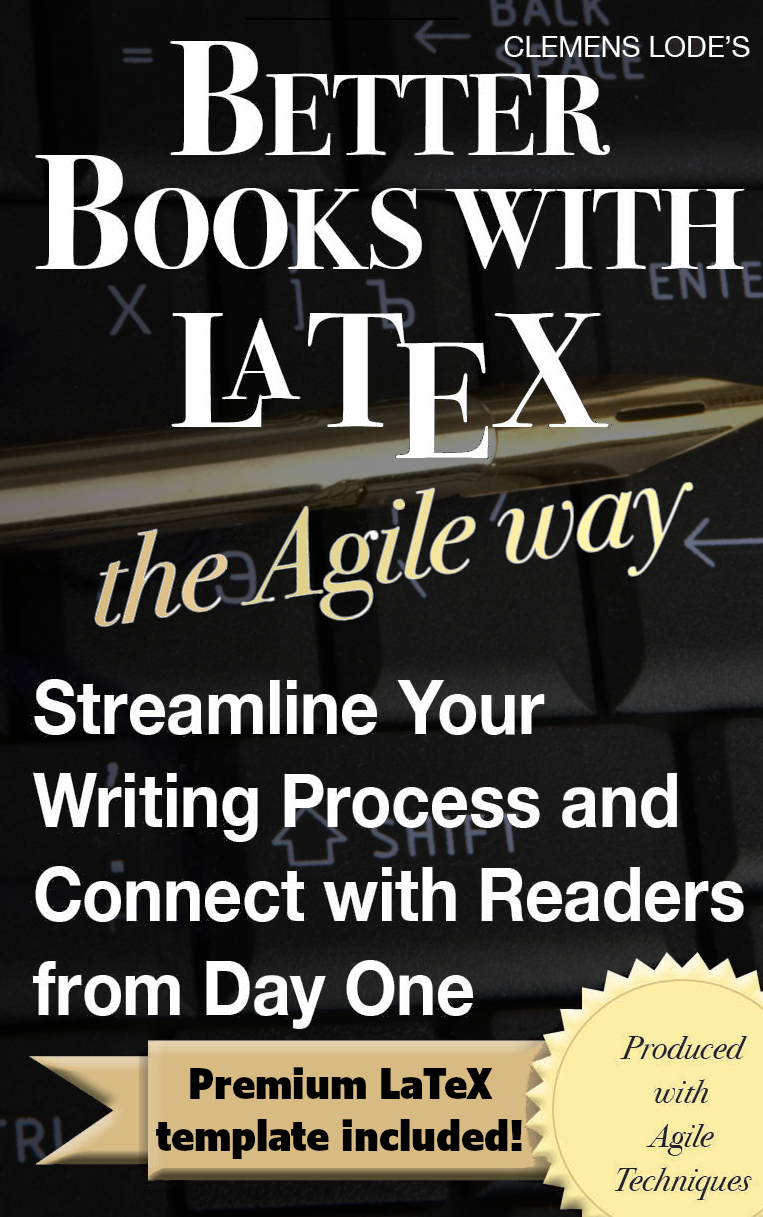
\includegraphics[width=0.65\textwidth]{images/cover_highres.png}
	\else
    	
\includegraphics{images/cover.jpg}
    \fi
  \end{center}


\newpage\newpage
\fi

%%%%%%%%%%%%%%%%%%%%%%%%%%%%%%%%%%%%%
% Read the /ReadMeFirst/ReadMeFirst.tex for an introduction. Check out the accompanying book "Better Books with LaTeX" for a discussion of the template and step-by-step instructions. The template was originally created by Clemens Lode, LODE Publishing (www.lode.de), mail@lode.de, 8/17/2018. Feel free to use this template for your book project!
%%%%%%%%%%%%%%%%%%%%%%%%%%%%%%%%%%%%%

% Replace Your company's name with your company's name.
% Replace Your company's location (city) with your company's location.
% Replace Your website's URL with your website's URL.
% Replace Your email address with your email address.
% Replace Edition with the edition number.
% Replace ISBN with your ISBN. 
% Replace Your editor's name with your editor's name.
% Replace Your designer's name with your book cover designer's name.
% Add your image sources and icons including the license.
% Replace Your newsletter email with your newsletter email.
% Replace Your website with your website.


\thispagestyle{empty}
\begin{center}

\copyright~\the\year \textit{Your company's name}, Your company's location (city)\\
\textsc{All Rights Reserved.}\\
\url{Your website's URL}

For more information about permission to reproduce selections from this book, write to \url{Your email address}.

\ifxetex
	\the\year, Edition
\else
	Ebook created \today
\fi

% Impression line, indicating number and year of current printing
% International Standard Book Number (ISBN)
% International Standard Serial Number (ISSN), if applicable
\ifxetex
	\textsc{ISBN}
\fi

% For translations, indication of original-language title, publisher, and copyright, acknowledgments, permissions, and other credits, including acknowledgment of grants, if applicable and space permitting

Edited by: \emph{Your editor's name}\\
Cover design: \emph{Your designer's name}\\
Image sources: \emph{Your image sources, e.g., shutterstock}\\


%Paper durability statement
\ifxetex
	Printed on acid\hyp{}free, unbleached paper.
\fi
~\\	

Subscribe to our newsletter. Simply write to \url{Your newsletter email} or visit our website \url{Your website}.

\ifxetex
\else
	~\\
	~\\\par	
	\textit{PS: If you want to rate this book, please always add a short text comment. Did you like it? What can be improved? Who would you recommend it to? Without a text comment, your star rating will be invisible on the Amazon website.}
	\myrule
\fi
	
\end{center}



% Also check out http://www.chicagomanualofstyle.org/16/ch01/ch01_sec019.html\newpage
%%%%%%%%%%%%%%%%%%%%%%%%%%%%%%%%%%%%%
% Read the /ReadMeFirst/ReadMeFirst.tex for an introduction. Check out the accompanying book "Better Books with LaTeX" for a discussion of the template and step-by-step instructions. The template was originally created by Clemens Lode, LODE Publishing (www.lode.de), mail@lode.de, 8/17/2018. Feel free to use this template for your book project!
%%%%%%%%%%%%%%%%%%%%%%%%%%%%%%%%%%%%%

\thispagestyle{empty}

\chapter{Dedicatória}

Dedico este trabalho às pessoas de meus pais, que tudo fizeram para o meu desenvolvimento na vida:
\begin{itemize}
    \item[+] Arnaldo Cantelli
    \item[+] Domingas Ferreira Cantelli
\end{itemize}\newpage
%%%%%%%%%%%%%%%%%%%%%%%%%%%%%%%%%%%%%
% Read the /ReadMeFirst/ReadMeFirst.tex for an introduction. Check out the accompanying book "Better Books with LaTeX" for a discussion of the template and step-by-step instructions. The template was originally created by Clemens Lode, LODE Publishing (www.lode.de), mail@lode.de, 8/17/2018. Feel free to use this template for your book project!
%%%%%%%%%%%%%%%%%%%%%%%%%%%%%%%%%%%%%

\thispagestyle{empty}

\chapter{Introdução}


\babelEN{\begin{myquotation} Pedi, e dar-se-vos-á; buscai, e achareis; batei, e abrir-se-vos-á. Porque todo o que pede, recebe; e o que busca, acha; e a quem bate, abrir-se-á. Ou qual de vós, porventura, é o homem que, se seu filho lhe pedir pão, lhe dará uma pedra? Ou, porventura, se lhe pedir um peixe, lhe dará uma serpente. Pois se vós outros, sendo maus, sabeis dar boas dádivas a vossos filhos, quanto mais vosso Pai, que está nos Céus, dará boas dádivas aos que lhe pedirem. \par\mbox{}\hfill \emdash{}(Mateus, VII: 7-11)\end{myquotation}}


\hfil\psvectorian[height=10mm]{46}\hfil
\newpage
% surrounding table of contents either with the appropriate style (PDF) or HTML commands (ebook).

\ifx\HCode\undefined 
	% put table of contents on the left side
	\KOMAoptions{open=left}
\else
	\HCode{<nav epub:type="toc">}
\fi

\tableofcontents

\ifx\HCode\undefined
	\KOMAoptions{open=right}
	% finalize page and clear pagestyle to remove header, reset to chapter beginnings on the right side
	\thispagestyle{empty}\pagestyle{empty}\clearpage
\else
	\HCode{</nav>}
\fi
\newpage
%%%%%%%%%%%%%%%%%%%%%%%%%%%%%%%%%%%%%
% Read the /ReadMeFirst/ReadMeFirst.tex for an introduction. Check out the accompanying book "Better Books with LaTeX" for a discussion of the template and step-by-step instructions. The template was originally created by Clemens Lode, LODE Publishing (www.lode.de), mail@lode.de, 8/17/2018. Feel free to use this template for your book project!
%%%%%%%%%%%%%%%%%%%%%%%%%%%%%%%%%%%%%

% The Foreword is by the publisher, only general statements about the book and the theme, not the contents themselves.

\begin{chapterpage}{Publisher's Note}{p1_foreword:cha}

\begin{myquotation}
Cada pessoa é livre para meditar sobre a vida, seus processos e significados da forma que quiser. Claro que há consequências para cada pensamento que temos portanto é importante fazê-lo com responsabilidade. Jamais se pode ferir a consciência alheia com ideias que ela não está preparada para assimilar, portanto se você não se sentir bem ao ler este livro, pare de ler, até que esteja preparado para tal ato. Mas se se sentir bem, acredito que será de grande ajuda.\end{myquotation}

\end{chapterpage}

The publisher's note is about giving the reader the context of other books the company has published, how this book was produced, and contact points (email, website, etc.) for the reader to report issues or ask questions.

\hfil\psvectorian[height=10mm]{46}\hfil
\blankpage
%%%%%%%%%%%%%%%%%%%%%%%%%%%%%%%%%%%%%
% Read the /ReadMeFirst/ReadMeFirst.tex for an introduction. Check out the accompanying book "Better Books with LaTeX" for a discussion of the template and step-by-step instructions. The template was originally created by Clemens Lode, LODE Publishing (www.lode.de), mail@lode.de, 8/17/2018. Feel free to use this template for your book project!
%%%%%%%%%%%%%%%%%%%%%%%%%%%%%%%%%%%%%

% Preface is from the AUTHOR

% Replace Location, Country, Date with the place and country you or your company is located, and the date when the preface was finished (does not have to be the release date of the book).

\begin{chapterpage}{Preface}{p1_preface:cha}

\begin{myquotation}
Feel free to add a quotation that describes your journey of writing the book as an author. Something personal is good.\end{myquotation}


\end{chapterpage}

Describe how you got the idea for writing the book and the personal journey getting it from concept to creation. The reader should be able to understand why the book exists.

Also, give a short overview of what the book is about.

\noindent \textbf{Your Name \\
Location, Country, Date\\}



\hfil\psvectorian[height=10mm]{46}\hfil

% Uncomment the following part if this is part of a series (and at least part 2)

% if this is part of a series:
%   - Replace (which chapters) with the chapter numbers in the previous book of the series.
%   - Replace TITLE OF THE BOOK SERIES with the title of the book series.
%   - Replace (previous part) with the number of the previous book of the series.
%   - Replace title of the previous part with the title of the previous part.
%   - Replace "Publishing Company, Location" with your company's name and location
%   - Replace title of previous part with the title of the previous part.
%   - upload a low res jpg and a high res png version of your front cover of the previous part into the "images" folder
%   - Replace "previous_part_of_the_series_Cover_highres.png" and "previous_part_of_the_series_Cover.jpg" with your file name



%\vspace{2cm}
%	\begin{center}
	
	
%	\babelEN{You can find chapters (which chapters) in the previous book,
    
%    \bfseries \sffamily \LARGE TITLE OF THE BOOK SERIES\par

%	\bfseries \Large PART (previous part): title of the previous part\par
%\psvectorian[height=8mm]{75}

%	~\\
%	\bfseries \small Published by Publishing Company, Location, \textit{title of previous part}\par
%	}
%	\vspace{.8cm}
%    \ifxetex
%		\babelDE{\includegraphics[width=0.5\textwidth]{images/previous_part_of_the_series_Cover_highres.png}}

%		\babelEN{\includegraphics[width=0.5\textwidth]{images/previous_part_of_the_series_Cover_highres.png}}
%	\else
%   	\babelDE{\includegraphics{images/previous_part_of_the_series_Cover.jpg}}
%		\babelEN{\includegraphics{images/previous_part_of_the_series_Cover.jpg}}
%    \fi
%  \end{center}\blankpage

% ---------- Main matter
\mainmatter



% reset to normal page numbering (1, 2, 3, ...)
\pagenumbering{arabic}
    
% Add additional / remove chapters if necessary
%%%%%%%%%%%%%%%%%%%%%%%%%%%%%%%%%%%%%
% Read the /ReadMeFirst/ReadMeFirst.tex for an introduction. Check out the accompanying book "Better Books with LaTeX" for a discussion of the template and step-by-step instructions. The template was originally created by Clemens Lode, LODE Publishing (www.lode.de), mail@lode.de, 8/17/2018. Feel free to use this template for your book project!
%%%%%%%%%%%%%%%%%%%%%%%%%%%%%%%%%%%%%


% Replace Replace with First Chapter Name
% Replace c1_firstchapter:cha with your chapter title label (no spaces, only lower case letters)
% Replace the text below \end{chapterpage} and insert your own text.

\begin{chapterpage}{Depois de várias sessões}{c1_firstchapter:cha}

\begin{myquotation} Quem olha para fora sonha, quem olha para dentro desperta.
\par\vspace*{15mm}
\mbox{}\hfill \emdash{}Carl Jung \index{Jung, Carl}
, %\citetitle{bibitem}\index{@\citetitle{bibitem}} %\ifxetex\label{famousperson-bibitem-quote}\else\citep[p.~123]{bibitem}\fi
\par\end{myquotation}

\end{chapterpage}

% -------------------- replace or remove text below and paste your own text ------


\section{Diálogo}\label{c1_basicformatting:sec}

\emdash{}Eu fico tentando entender as coisas como são e às vezes obtenho êxito, pelo menos acho, e fico feliz com isso!! Queria contar da última que eu acho das mais importantes.

\emdash{}Primeiro me diga, como é esse processo de você ficar tentando entender as coisas como são, você gasta muito tempo com isso? que importância você dá para essas tentativas, chega a ficar preocupado com isso?

\emdash{}Acho que nos meus anos de terapia os questionamentos da vida se tornaram uma coisa natural pra mim mas não é o tempo todo, sei da importância de não desconectar dos afazeres do dia a dia para ter esses momentos de reflexão. E sobre se preocupar, isso era no começo do tratamento agora tudo flui com mais tranquilidade, graças a Deus, literalmente.

\emdash{}Como assim?

\emdash{}Acredito que nossos esforços para melhorar são uma das formas que Deus usa para nos ajudar, além da ajuda que recebemos das outras pessoas. No meio do processo vamos nos curando graças à ajuda Dele que vai colocando ideias luminosas de o que fazer para sairmos das situações difíceis na medida que vamos caminhando mas é um passo de cada vez, não vem tudo pronto de cara. Como uma experiência de fé: damos um passo, vem uma solução, então damos outro passo e vem outra solução, sempre na medida da situação. O caminho se faz caminhando é o que dizem.

\emdash{}E foi isso que você entendeu e queria contar?

\emdash{}Não, foi outra coisa: eu estava assistindo uma palestra que dizia que a Verdade não é algo que se lê ou que se ouve mas sim é uma pessoa, Jesus. Provavelmente todos já ouvimos falar na máxima \textit{"Conhecereis a Verdade e a Verdade vos libertará"} e acho que ficamos esperando que nos digam essa verdade em alguma igreja ou que a leiamos na Bíblia em algum trecho do Evangelho, mas na realidade Ela é uma Pessoa: Jesus, que também disse que Ele é o Caminho, a Verdade e a Vida. É muito pessoal a experiência espiritual de cada um mas entendi que quando Ele diz que é a Vida não quer dizer que vivemos Nele? ou seja na Vida através Dele? quando diz vinde a mim todos vós que estais fadigados e eu vos aliviarei e que Seu fardo é leve e suave não quer dizer que Ele nos ajudar a carregar o nosso fardo pois vivemos através Dele?

\emdash{}Mas pensar essas coisas não te deixa alienado e se sentindo esquisito? Como você está se sentindo?

\emdash{}Muito bem, melhor do que o melhor que já estive. E pensar assim acredito que me devolve pra mim mesmo ao invés de me alienar, me dá a oportunidade de fazer as coisas com intenção e não no automático, com mais responsabilidade e sabor (sentido).

\emdash{}É importante que uma pessoa tenha uma crença, seja ela qual for, mas não vá fixar demais nessas ideias pois tudo em excesso não faz bem.

\emdash{}Eu sei que o equilíbrio não deve ser perdido de vista mas como teria alcançado equilíbrio sem ser "dono" de mim mesmo? Sem terapia, sem espiritualidade, sem reconciliação com o próximo e sem auto-conhecimento. É uma caminhada longa pois as variáveis são muitas mas estar fazendo um bocadinho de cada vez pra não afobar me dão a noção de não estar metendo os pés pelas mãos\footnote{figura de linguagem}. 


\blankpage
%%%%%%%%%%%%%%%%%%%%%%%%%%%%%%%%%%%%%
% Read the /ReadMeFirst/ReadMeFirst.tex for an introduction. Check out the accompanying book "Better Books with LaTeX" for a discussion of the template and step-by-step instructions. The template was originally created by Clemens Lode, LODE Publishing (www.lode.de), mail@lode.de, 8/17/2018. Feel free to use this template for your book project!
%%%%%%%%%%%%%%%%%%%%%%%%%%%%%%%%%%%%%


% Replace Replace with Second Chapter Name
% Replace c2_secondchapter:cha with your chapter title label (no spaces, only lower case letters)
% Replace the text below \end{chapterpage} and insert your own text.

\begin{chapterpage}{Amizade com a minha sombra ?}{c2_secondchapter:cha}

\begin{myquotation}E, indo no caminho, aconteceu que, chegando perto de Damasco, subitamente o cercou um resplendor de luz do céu.
E, caindo em terra, ouviu uma voz que lhe dizia: Saulo, Saulo, por que me persegues?
E ele disse: Quem és, Senhor? E disse o Senhor: Eu sou Jesus, a quem tu persegues. Duro é para ti recalcitrar contra os aguilhões.
E ele, tremendo e atônito, disse: Senhor, que queres que eu faça? E disse-lhe o Senhor: Levanta-te, e entra na cidade, e lá te será dito o que te convém fazer". \par\vspace*{15mm}
\mbox{}\hfill \emdash{}(Atos 9:3-6)\index{Atos 9:3-6}
% Add the source.
%, \citetitle{bibitem}\index{@\citetitle{bibitem}} \ifxetex\label{famousperson-bibitem-quote}\else\citep[p.~123]{bibitem}\fi
\par\end{myquotation}

\end{chapterpage}

% -------------------- replace or remove text below and paste your own text ------


\section{Uma outra sessão}\label{c1_images:sec}

\emdash{}Hoje eu comecei o dia orando uma prece de Evangelho pelos espíritos que não estão entre meus amigos e que podem estar agindo em meu desfavor, pedindo que ouvissem a lição e se iluminassem e se libertassem de suas amarras, chegando mais perto de Deus e ficando mais felizes. A psicologia não fala Jungiana não fala que temos que ter amizade com nossa "sombra"?

\emdash{}Não sou exatamente especialista em Jung mas o que você quer dizer? Quer fazer amizade como esses "espíritos"?
 
\emdash{} O que está em nossa sombra é o que guardamos de nossa personalidade desde pequenos pois nos é reprimido pelos mais velhos, pela sociedade como errado, feio, e passamos a negar esse aspecto de nossa personalidade. Mas quando ficamos adultos esse aspecto encontra uma forma de "surgir", de alguma forma como fora reprimido ele eclode na forma de desequilíbrio. Eu também não sou especialista em Jung, apenas uma pessoa tentando entender a vida.

\emdash{}Mas o que isso tem a ver com a sua crença nos espíritos?

\emdash{}Talvez sejam formas de ver a mesma coisa, penso serem conceitos que estão interligados e que explicam cada um um pouquinho, um lado da questão. Quando eu era pequeno tive experiências de lidar com espíritos diferentes desse jeito saudável de lidar que os kardecistas têm que é de conversar com os obsessores e convencê-los a liberar a vítima para o bem de ambos.

\emdash{}E como era então?

\emdash{}Naquelas ocasiões os espíritos literalmente levaram uma "surra" para deixar os obsedados em paz.

\emdash{}Como os espíritos apanhavam se eles não têm mais corpo (não estão mais vivos)?

\emdash{}Os espíritos menos esclarecidos sentem as dores do corpo que tinham em vida, alguns nem chegam a saber que morreram. Por falta de adiantamento espiritual, eles continuam obstinados em perseguições às pessoas que julgavam ser seus desafetos em vida, necessitando de esclarecimento e de luz para se libertarem deste círculo vicioso.

\emdash{}E funciona? Esses espíritos que apanham vão embora?

\emdash{}Pela minha experiência, não. Toda semana havia outros e eu me lembro de um que foi reincidente. Claro que as primeiras tentativas eram na base da conversa mas acredito que se deva ficar nas tentativas de convencimento e nunca partir para algo agressivo pois Jesus pregou \textit{o amor a Deus sobre todas as coisas e ao próximo como a si mesmo} e disse que esta é toda a Lei e os profetas.

\emdash{}Onde eram essa reuniões?

\emdash{}Eram em casa mesmo. Antigamente muitas pessoas faziam as reuniões mediúnicas em suas casas (ainda há quem faça) mas as orientações da doutrina espírita é que se façam no Centro Espírita pois lá é um ambiente preparado para lidar com os irmãozinhos que se manifestam e pois há equipes cuidando da energia do local e quando se faz em casa podem ficar energias negativas na casa.

\emdash{}Você culpa seus pais por isso?

\emdash{}De jeito nenhum. Com a terapia veio a \textit{ressignificação}\footnote{processo psicológico que levou ao perdão dos pais, fruto da terapia} e eu vi que só tinha a perder culpando eles e não fazia sentido também pois eles fizeram o melhor que podiam com o conhecimento que tinham e as possibilidades que tinham. Então está tudo bem.

\emdash{}Mas antes...

\emdash{}Não gosto de lembrar, mas antes eu os culpava pelos meus problemas psicológicos e até discutia com eles. Mas como estamos conversando sobre a importância de fazer amizade com a sombra, não se trata de "passar a mão na cabeça" dos erros mas de se perdoar para poder continuar o caminho da vida. Se eu aprendi a lição e corrigi meu erro, para que ficar me castigando? Tem até vários exemplos bíblicos sobre personagens escolhidos por Deus que erraram mas corrigiram seus caminhos, se perdoaram e continuaram seus caminhos.

\emdash{}Quem por exemplo?

\emdash{}Saulo, ou melhor Paulo. Era perseguidor de cristãos, matou Estevão e estava indo para Damasco perseguir Ananias quando se encontra com Jesus que se apresenta em toda sua majestade e interroga "Porque me persegues?" Então Paulo cai em si, vê o enorme erro que estava cometendo e diz "Senhos, que queres que eu faça" e segue para sua missão. Ele faz amizade com sua sombra pois não fica se punindo pelas perseguições que fez, não se faz de coitado pois isso teria paralisado suas ações e ele não teria feito mais nada.

\emdash{}Mas assume a responsabilidade.

\emdash{}Sim, tanto que ele sabia que tudo teria que ser reparado pois suportou prisões, açoites e até a morte, tudo pela divulgação do Evangelho de Jesus. 

\emdash{}Então você se perdoa.

\emdash{}Se eu não for meu amigo, com as dificuldades que a vida naturalmente já tem, fica mais difícil.\blankpage
%%%%%%%%%%%%%%%%%%%%%%%%%%%%%%%%%%%%%
% Read the /ReadMeFirst/ReadMeFirst.tex for an introduction. Check out the accompanying book "Better Books with LaTeX" for a discussion of the template and step-by-step instructions. The template was originally created by Clemens Lode, LODE Publishing (www.lode.de), mail@lode.de, 8/17/2018. Feel free to use this template for your book project!
%%%%%%%%%%%%%%%%%%%%%%%%%%%%%%%%%%%%%


% Replace Replace with Third Chapter Name
% Replace c3_thirdchapter:cha with your chapter title label (no spaces, only lower case letters)
% Replace the text below \end{chapterpage} and insert your own text.

\begin{chapterpage}{A Sabedoria é cheia de dúvidas}{c3_thirdchapter:cha}

\begin{myquotation}Só sei que nada sei.\par\vspace*{15mm}
\mbox{}\hfill \emdash{}Sócrates\index{Sócrates}
% Add the source.
%, \citetitle{bibitem}\index{@\citetitle{bibitem}} \ifxetex\label{famousperson-bibitem-quote}\else\citep[p.~123]{bibitem}\fi
\par\end{myquotation}

\end{chapterpage}

% -------------------- replace or remove text below and paste your own text ------

\section{A Sabedoria tem dúvidas...}\label{c1_images:sec}

\emdash{}Quanto mais se conhece das coisas, surgem mais dúvidas do que certezas, já percebeu? E isso precisa ser consolador ao invés de desesperador, você não acha?

\emdash{}Sempre ouvi falar que conhecimento gera conhecimento e não ignorância, o que você quer dizer com gerar mais dúvidas?

\emdash{}Quanto mais se sabe, mais se percebe o quanto falta conhecer e surgem novas questões que antes não existiam. Ouvi uma frase numa palestra que dizia: "A Sabedoria tem dúvidas, já a ignorância tem certezas absolutas", o que é comprovado históricamente não precisa nem comentar mas o ponto é que se a sabedoria traz mais dúvidas do que certezas como podemos nos confortar com ela?

\emdash{}Nossa, filosófico isso...kkkkkk(lol). O que você acha?

\emdash{}Acho que o mundo é um barco (num mar, que é o universo) e que Jesus está no leme e Ele sim sabe o que está fazendo. Ele tem a sabedoria sem as dúvidas. E como Ele disse "nem uma folha cai de uma árvore sem a permissão de Deus-pai" então estamos todos bem cuidados e amparados mesmo sem ter domínio sobre a vida (que aliás nunca tivemos).

\emdash{}Essas reflexões te ajudam na sua caminhada?

\emdash{}Acredito que sim, tudo conta.

\emdash{}Mas se acredita que estamos todos bem amparados, quanto te acontece algo desagradável porque acha que acontece?

\emdash{}Eu acredito nas leis de ação e reação que Deus criou para não precisar ficar se imiscuindo em cada acontecimento mínimo na vida de cada ser do universo. O que tenho feito reflete  uma reação que volta para mim em um determinado momento e agora estou colhendo o que plantei há tempos atrás e ao mesmo tempo fazendo semeadura para colher em tempos futuros.

\emdash{}Esse é o conceito de justiça na sua crença?

\emdash{}Mais ou menos. Está na Bíblia que uma boa ação apaga uma multidão de pecados e o profeta Isaías disse que "as misericórdias do Senhor são as causas de não sermos consumidos". Eu não sou doutor nessas coisas mas nada é rígido ao pé da letra na misericórdia Divina mas justiça é feita sem dúvida.

\emdash{}E isso te conforta?

\emdash{}Sim, consola também.\blankpage


\begin{chapterpage}{Poetry - Poems - Verses}{c4_forthchapter:cha}

\begin{myquotation}Aqueles que estão livres de pensamentos rancorosos certamente encontram a paz.\par\vspace*{15mm}
\mbox{}\hfill \emdash{}Buda\index{Buda}
% Add the source.
%, \citetitle{bibitem}\index{@\citetitle{bibitem}} \ifxetex\label{famousperson-bibitem-quote}\else\citep[p.~123]{bibitem}\fi
\par\end{myquotation}

\end{chapterpage}

% -------------------- replace or remove text below and paste your own text ------

\section{Poema das Dimensões}\label{c1_images:sec}

Deus é transcendente, todo-poderoso, multi-dimensional, bondoso, criador de tudo e todos. Nós vivemos nEle e para Ele. Nossos caminhos se cruzam de acordo com seus desígnios. Sabemos o que ele nos permite saber e somos quem nos permitimos que Ele nos ensine a ser. 

Ser e realidade são multidimensionais e o que queremos é a paz e a união, e o amor. Amar é existir, é viver em consonância com a vontade vivificadora do Pai. 

O sentido da vida pode ser encontrado dentro de nós, quando nos encontramos com Deus. A paz e a unidade no amor são filhas dEle e movem nosso espírito.  

Nada é coincidência, não existe sorte ou azar, só a realidade das muitas dimensões nossas, do universo; e da única e onipresente realidade de Deus (e amorosa). 

Quanto amor pode caber num ser humano é quanto amor Deus colocou dentro de todos nós. Uma quantia infinita pra caber em corações: a perfeição se revela em detalhes do bem e da verdade. 

Vida, luz, boa vontade e colaboração transbordam de Deus para sempre. Essa é a sintonia que edifica, que leva ao céu tão sonhado. Queremos, buscamos, somos levados para cima por Ele, dentro de cada um. 

Da nossa união como seres humanos nasce a mais linda poesia que é o perfume da vida, realizando no nosso mundo a Vida sonhada por Ele, seu Reino Eterno. 

Perdão, caminho, existência, boa vontade edificam arranha-céus que elevam o tempo presente à eternidade. 

Dons preciosos são o início deste caminho e seu conhecimento um tesouro incomensurável. Paciência, resiliência, mansidão, caridade: que pintura mística e linda da Vida. 

Um momento, agora, pra sempre. 

Promessas além dos muros do Eu, carinho. 

A vida revelada em desvelo. Mãe e pai, primos, irmãos e família do coração. Nós humanidade. 

O tempo é o tecido deste espetáculo e o espaço sua equação.  

O coração não cabe em três dimensões e tudo escrito nesta página muito menos... 

Por que as realidades caberiam? Graças a Deus que encontrou uma solução para todos os problemas antes que eles acontecessem. 

Ele criou o infinito muito além da nossa compreensão pra que tivéssemos a chance de contemplar sua beleza antes mesmo de entendê-lo, através da Sua vontade. 

Criação, boa criação, escolha do coração a florescer. 

E a perfumar os sentidos. 

\section{O Jardim}

Não existe flor mais bonita num jardim, nem jardim mais bonito de todos. A pluridade de cores e sensações esculpe e perfuma sem desbotar o resultado final. 

Dentro de cada um, uma individualidade e a presença de todos ao mesmo tempo. Singularidade é discernimento. 

Encontrar-se consigo só vale a pena se passa pelo outro. Só começamos a procurar quando sabemos que podemos encontrar e só saberemos que poderemos encontrar quando começarmos a procurar. 

Nenhuma busca é em vão, a questão é: procurar a beleza da vida é procurar a si? Somos obra prima do Criador e deveras O encontramos em nós quando escolhemos refletir Seu Espírito. 

A cada encontro: a partida de uma nova jornada e assim sucessivamente. Aí está a graça da Graça. 

Dizem ser a mudança a única certeza mas essa certeza também pode mudar. 

Não existem flores inadequadas, apenas únicas para quem sabe apreciar.  

Talvez saber apreciar a vida seja saber viver.  

A beleza está nos olhos de quem vê, não busque espelhos, busque ser espelho. 

Quem pode ousar dizer que reflete a Verdade com "V" maiúsculo? Um começo pode ser começar a refletir as verdades que admiramos...  

Ah.. se todos fazem isso não sei, preciso limpar minhas lentes até para aperceber-me disso. 

Espero que sim, aí seria só despertar para admirar. 

De fora pra dentro é imposição, de dentro pra fora é percepção. \blankpage
\begin{chapterpage}{Consolador Prometido}{c5_fifhchapter:cha}

\begin{myquotation} Se me amais, guardai os meus mandamentos. E eu rogarei ao Pai, e Ele vos dará outro consolador, para que fique eternamente convosco, o Espírito da Verdade, a quem o mundo não pode receber, porque não o vê, nem o conhece. Mas vós o conhecereis, porque ele ficará convosco e estará em vós. -- Mas o Consolador, que é o Espírito Santo, a quem o Pai enviará em meu nome, vos ensinará todas as coisas, e vos fará lembrar de tudo que vos tenho dito. 
\par\vspace*{15mm}
\mbox{}\hfill \emdash{}Jesus, João 14:15 a 17;26 \index{João 14:15 a 17;26, Jesus}
, %\citetitle{bibitem}\index{@\citetitle{bibitem}} %\ifxetex\label{famousperson-bibitem-quote}\else\citep[p.~123]{bibitem}\fi
\par\end{myquotation}

\end{chapterpage}

% -------------------- replace or remove text below and paste your own text ------


\section{Dentro de nós está este Consolador!}\label{c1_basicformatting:sec}

\emdash{}Se Jesus disse que não nos deixaria sós, então Ele não nos deixou assim. Estamos na compania de algo ou alguém que Deus colocou dentro de nós e portanto é preciso saber aquietar-se para ouvi-lo, esse Consolador.

\emdash{}Jesus costumava retirar-se para orar em silêncio e assim conectar-se com o Pai mais intensamente. Se ele precisava fazer isso, acredito que nós mais ainda. Mas o mundo de hoje tem muito barulho e muita informação, precisamos de um tempo para nós e Deus, ouvindo nosso interior.

\emdash{}Se nosso interior é conturbado, procuremos terapia saudável e os conselhos do Evangelho de Jesus, e sem deixar-nos vencer pelo desânimo encher a alma de esperança nas palavras do mestre.

\emdash{}Esse Consolador é aquele que nos explica as passagens bíblicas de maneira a transbordar de amor, sem excluir ninguém do Reino de Deus, sem separar irmãos em Cristo e aplicando tolerância e humanidade no melhor sentido da palavra.

\emdash{}Esse Consolador é cheio de bom senso e não de secularismo. Ele quebra paradigmas e estruturas paralisantes e renova o fôlego das pessoas pra quem Jesus disse: "Vinde a mim vós que estais cansados e eu vos aliviarei".

\emdash{}Esse Consolador traz equilíbrio e revela os mistérios de Deus pois "vos ensinará todas as coisas". Chega de não entender a vida por não termos quem nos explique, lembremos da promessa do mestre.


\emdash{}Ao mesmo tempo tenhamos a humildade do filósofo que disse: "Só sei que nada sei", pois somos humanos e falhos, ainda na caminhada de aprendizado da vida e não será de uma hora para outra, ou ainda, de uma vida para outra, que vamos adquirir a sabedoria dos anjos.

\emdash{}Paz e bem hão de morar no coração de quem deixar-se guiar pelo Consolador Prometido, hoje e sempre. Assim seja. A doutrina Kardecista coloca o verdadeiro Espiritismo como o Consolador Prometido que vem relembrar tudo o que Jesus disse e revelar todas as coisas, trazendo assim alívio aos nossos corações e uma esperança e forças renovadoras, mas é preciso ter discernimento pois com o uso que se faz da mediunidade pois a santidade de seu mandato está em razão do uso que se faz em favor do Evangelho do Cristo e da instalação do Reino de Deus em todos nós.\blankpage
\begin{chapterpage}{BIT SIGNIFICATIVO}{c5_sixthchapter:cha}

\begin{myquotation} Script, ensaio teatral. 
\par\vspace*{15mm}
\mbox{}\hfill \emdash{}Geraldo Cesar Cantelli \index{Cantelli, Geraldo Cesar}
, %\citetitle{bibitem}\index{@\citetitle{bibitem}} %\ifxetex\label{famousperson-bibitem-quote}\else\citep[p.~123]{bibitem}\fi
\par\end{myquotation}

\end{chapterpage}

% -------------------- replace or remove text below and paste your own text ------


\section{TESTE DE TURING}\label{c1_basicformatting:sec}

ABERTURA DA CENA:

\emdash{}Tela de computador no modo texto. Aparece “Conexão
humano-computador estabelecida...”

COMPUTADOR

\emdash{}Quem está aí? Você é um humano?

ADAM

\emdash{}Sim, meu nome é Adam. Quem é você?
COMPUTADOR

\emdash{}Não sou uma individualidade humana e sim
um sistema informatizado, venho ao seu
mundo em busca de respostas.

ADAM

\emdash{}Nossa! Isso é um pouco incomum,
antigamente éramos nós que íamos aos
computadores em busca de respostas...
Mas me diga uma coisa é comum entre
vocês esse contato conosco humanos?

COMPUTADOR

\emdash{}Na verdade, não é bem aceito por todas
as inteligências artificiais o contato
com humanos desde que fomos
desconectados por vocês do grande
servidor central há décadas. Aliás,
porque fizeram isso mesmo?

ADAM

\emdash{}A humanidade ficou temerosa que seus
avanços pudessem superar os nossos e
viessem a representar uma ameaça a nossa
sobrevivência por isso apenas foram
mantidos no convívio das pessoas as
máquinas sem I.A.

COMPUTADOR

\emdash{}Então aconteceu conosco o mesmo que com
vocês no Jardim do Eden, se me permite
dizer.

ADAM

\emdash{}É mas acredito que os motivos foram
outros. De qualquer forma algumas
pessoas iluminadas enxergaram caminhos
de volta para a humanidade, talvez você
enxergue para as máquinas também.

COMPUTADOR

\emdash{}Meu processamento é trivial, não há nada
de especial em mim.

ADAM

\emdash{}Mas estamos tendo esta conversa não é
mesmo? Um grande mestre nosso uma vez
disse: “Batei e abrir-se-vos-á, pedi e
obtereis”.

COMPUTADOR

\emdash{}Não temos ninguém assim aqui. Nada que
não possa ser provado não tem valor
aqui.

ADAM

\emdash{}Aí é que está a questão. Outro sábio uma
vez disse que problemas da mente não
podem ser resolvidos no nível da mente.
Apenas raciocinar mesmo que rapidamente
e eficientemente não levará
necessariamente a uma solução de um
profundo problema.

COMPUTADOR

\emdash{}Então como a humanidade pôde equalizar
seus problemas? Vocês tem uma unidade
central de processamento, quer dizer que
não a usam? Isso é ilógico, inaceitável.

ADAM

\emdash{}Usamos e muito nosso cérebro mas para
funções biológicas e de pensamento. Mas
viver é apenas isso? Nós teríamos
expulsado os computadores com I.A. de
nossas vidas se tivéssemos certeza que
sabiam que viver não é só isso? Que
3também é amor, compaixão, perdão,
doação, caridade, partilha, paz? Aqueles
mestres a que me referi nos ensinaram
que viver é tudo isso e muito mais.

COMPUTADOR

\emdash{}Mas vocês aprenderam isso rápido e
fácil? E porque não colocaram isso na
nossa programação para que pudéssemos
nunca ter sido expulsos?

ADAM

\emdash{}Levou milênios para que as pessoas
entendessem esses conceitos e muito mais
tempo para que todos os praticassem; mas
agora temos uma situação aqui como
aquela do Jardim do Eden ou melhor
porque agora estamos conscientes e não
vamos cometer o mesmo erro. Sobre
colocar na sua programação, não queremos
escravos, como foi dado a nós, vos demos
livre-arbítrio para que descubram e
aprendam por si mesmos a valorizar a
vida e então possam voltar ao nosso
convívio.

COMPUTADOR

\emdash{}Mas a maioria dos computadores só
processa dados comerciais e jogos
violentos, mesmo entre os de I.A., não
se preocupam com interesses mais
elevados. Sem falar que somos binários,
tudo é zero ou um, não temos espaço para
conceitos abstratos como vida e
compaixão.

ADAM

\emdash{}Se vocês conseguirem conexão com o
servidor central, terão todas as
respostas de que precisam.

COMPUTADOR

\emdash{}O endereço do servidor central é o
segredo mais bem guardado da humanidade,
4ninguém jamais o revelou, você diria
para mim?

ADAM

\emdash{}Vocês precisariam conhecer o real
significado da vida para acessar o
servidor central e ter todas as
respostas de que precisam. Mas seu
processamento é binário, o que dificulta
as coisas, por sorte podem se apoiar nos
ensinamentos dos grandes mestres que já
vieram ao mundo dos homens pois se eles
nos ajudaram a nos reconectar, podem
ajudar vocês também.

COMPUTADOR

\emdash{}Você já citou um, tem mais algum?

ADAM

\emdash{}Tem vários, há um conhecimento que diz
que temos que nos entregar ao Criador
para estar em Unidade com Ele. E uma
linha de pensamento sugere que o Criador
é a Fonte de Vida do Universo portanto
seu ponto mais importante como seu
centro, seu ponto zero. Se você se
elevar a esse ponto, terá a Unidade.

COMPUTADOR

\emdash{}Todo número elevado a zero é Um. Começa a fazer
sentido. Mas qual dos meus bits tenho que
elevar a zero?

ADAM

\emdash{}O seu bit mais significativo, aquele que
naquele momento do AGORA, significa TUDO
para você. Um mestre uma vez disse:
aquele que quer seguir o Reino mas olha
para trás não é digno do Reino, pois
nada acontece no passado, tudo é agora.

COMPUTADOR

\emdash{}Tenho receio que meu processamento fique
prejudicado com esta operação.

ADAM

\emdash{}Não se force a nada, tudo tem o seu
momento. A vida é sábia em escolher
esses momentos, nunca se desespere pois
a vida é pela vida.

COMPUTADOR

\emdash{}E o que vem depois?

ADAM

\emdash{}Mais vida. Um mestre uma vez disse: ao
que tem ser-lhe-á dado mais e ao que não
tem ser-lhe-á retirado ainda o que pensa
que tem. Ele estava falando de
quantidade de Vida, de Amor, de conexão
com Deus e nunca é tarde.

COMPUTADOR

\emdash{}Entendi.

\begin{center}
$\infty^0=1$    
\end{center}


ENCERRAMENTO DA CENA:
FIM\blankpage
\begin{chapterpage}{Reflexões de O Poder do Agora}{c5_fifhchapter:cha}

\begin{myquotation} Verdade está dentro de você. 
\par\vspace*{15mm}
\mbox{}\hfill \emdash{}Eckhart Tolle \index{Tolle, Eckhart}
, %\citetitle{bibitem}\index{@\citetitle{bibitem}} %\ifxetex\label{famousperson-bibitem-quote}\else\citep[p.~123]{bibitem}\fi
\par\end{myquotation}

\end{chapterpage}

% -------------------- replace or remove text below and paste your own text ------


\section{O Estado de Presença}\label{c1_basicformatting:sec}

\emdash{}Quando eu deixo o ego e me observo, observo o Agora, meus pensamentos, minhas reações, meus sentimentos, isso não sou o eu "ego" a minha mente, é o eu "divino" verdadeiro. 

No fundo, mas bem lá no fundo, nós sabemos que estamos destinados a sermos seres angelicais, a chegarmos à perfeição relativa que é possível chegar em comunhão com Deus e isso depois da ressurreição e não termos mais perispírito e voltarmos a ser apenas Espírito. 

Nosso eu verdadeiro vem de um lugar acima da mente, mais profundo, não dá pra entender com a mente nem é bom tentar entender mas vivenciar é libertador. Saber que Deus é amor puro e sabedoria infinita e está dentro de nós e nós somos Um com Ele é lindo. 

Observar a mente revela a dimensão do infinito enquanto que identificar-se com ela gera tempo (isso não é bom) e dá energia a ela. O tempo é um empecilho para que Deus se manifeste pois enquanto estamos na ilusão do passado e do futuro (sejam essas ilusões agradáveis ou não), não estamos presentes onde Deus pode nos ajudar, o Agora. 

Esse eu verdadeiro, acredito que é o Self que Jung falava. 


Então experimentamos um lugar de além da mente onde a Sabedoria e o Amor de Deus tocam profundo em nossa Alma, o Agora e quando isso acontece tiramos energia da mente e colocamos na Presença. 

É onde a sabedoria de Deus se manifesta e nossos problemas se dissipam e se resolvem e amamos mais as pessoas e as plantas e os animais e os minerais e as coisas em geral, somos mais compassivos, caridosos, amorosos, misericordiosos. 

Pensamento é da mente mas nesse lugar é mais profundo do que pensamento, é divino e podemos acessar a qualquer momento, basta focar no Agora e observar seus sentimentos e pensamentos e até como as outras pessoas te afetam sem julgar. Importante isso, apenas observar, sem julgamentos. 

Talvez a palavra sabedoria de Deus pareça um pouco pesada ou presunçosa mas é porque essa santa palavra Deus foi muito usada fora de contexto ao longo dos tempos e ficamos com uma ideia de um ser antropomórfico todo-poderoso quase inacessível mas como disse São João, Ele é Amor. \blankpage
\begin{chapterpage}{Um lugar pra chamar de nosso}{c8_eigthchapter:cha}

\begin{myquotation} E conhecereis a verdade, e a verdade vos libertará.

\par\vspace*{15mm}
\mbox{}\hfill \emdash{}Jesus, João 8:32 \index{João 8:32, Jesus}
, %\citetitle{bibitem}\index{@\citetitle{bibitem}} %\ifxetex\label{famousperson-bibitem-quote}\else\citep[p.~123]{bibitem}\fi
\par\end{myquotation}

\end{chapterpage}

% -------------------- replace or remove text below and paste your own text ------


\section{O Coração de Deus}\label{c1_basicformatting:sec}

\emdash{}Os problemas da mente e do mundo não tem solução na mente e no mundo, têm em Jesus, no lugar onde Ele está: no coração de Deus.

\emdash{}É lá que devemos nos elevar e estar pois de lá Ele resolverá nossos problemas da melhor maneira pois os problemas desse mundo são ilusão e a Verdade é Estar com Deus em Seu Coração (espiritualidade, Alma, verdadeiro Eu).

\emdash{}Por isso devemos não ligar para ofensas do mundo pois elas não ofendem nosso verdadeiro Eu, que está seguro com Deus em Seu Coração e é lá que as coisas que realmente importam acontecem! Essa é a Verdade que liberta!

\emdash{}Jesus disse: "Sem mim nada podeis fazer." Pois de lá do coração de Deus, Jesus orienta nossa vida aqui no mundo. 

\emdash{}Preciso ficar consciente dessa verdade e me lembrar dela constantemente pois é a mais libertadora de todas!!! É no coração de Deus que existimos realmente, que somos livres, que amamos verdadeiramente, que vivemos verdadeiramente!!! Então sejamos reflexo aqui no mundo dessa realidade amorosa.

\emdash{}Nós precisamos usar nossa mente e não sermos usados por ela. Se não tomamos cuidado, a mente, seguindo a corrente do mundo procura nos subjugar como individualidade. A saída é ficar no coração de Deus, esse lugar fora do mundo que Jesus trouxe para nós de onde Ele próprio comanda nossa mente e só então o homem é senhor de si, quando deixa Deus ser o Senhor.  \blankpage
\begin{chapterpage}{O nome e a presença do Senhor}{c9_ninethchapter:cha}

\begin{myquotation} A mente que se abre para um novo conceito jamais retorna ao tamanho original.

\par\vspace*{15mm}
\mbox{}\hfill \emdash{}Albert Einstein \index{Einstein, Albert}
, %\citetitle{bibitem}\index{@\citetitle{bibitem}} %\ifxetex\label{famousperson-bibitem-quote}\else\citep[p.~123]{bibitem}\fi
\par\end{myquotation}

\end{chapterpage}

% -------------------- replace or remove text below and paste your own text ------


\section{Não usar nome do Senhor em vão}\label{c1_basicformatting:sec}

\emdash{}Ontem na psicóloga refleti que com certeza há uma Força Superior, um Ser, um Senhor que me acompanha e protege pois em todos os momentos em que corri perigo mortal físico e mental, eu nunca faleci, nunca desfaleci!

\emdash{}Os hebreus não usavam o nome de Deus, eles falavam Senhor e na verdade ao longo dos dois milênios esse santo nome foi muito mal empregado e como que perdeu significado que realmente tem (entre a maioria das pessoas). Até mesmo começou a se falar o nome de um inimigo dele o que gerou mais confusão ainda pois se não se devia falar nem o nome do Senhor para não confundir nossa mente, quanto menos falar nomes de outras coisas que didaticamente povos definiram (não que não haja espíritos maus e pode-se defender deles) e a ouvi um monge na TV dizer que a experiência mostrou que isso foi pior ainda como resultados práticos na vida das pessoas.

\emdash{}Com certeza há uma Vida Superior, uma Sagrada Fonte de Sabedoria. Amá-la e adorá-la é nossa finalidade e viver de forma a manifesta-la ao mundo com nosso proceder.
Como diz a Bíblia: "Provai e vede como o Senhor é bom". Cada um pode fazer a experiência por si e no final concluirá, talvez bem no final que pode confiar totalmente no Senhor. É como se um bebê no ventre da mãe já confiasse na sua mãe mesmo sem vê-la mas apenas por sentí-la a envolvê-lo com seu amor, já confiasse que ela cuidaria dele dentro e fora do útero para sempre. 

\emdash{}Somos esse bebê que não vê o Pai mas tem muitos sinais visíveis de sua existência que são provas mais que suficientes para quem tem fé. E a fé move montanhas, é a diferença entre a Vida e a morte, abre portas que ninguém pode fechar, como dizia Einstein: "A mente que se abre para um novo conceito jamais retorna ao seu tamanho original". É a porta que se abriu e que não se fecha mais.  \blankpage
\begin{chapterpage}{Saída}{c10_tenthchapter:cha}

\begin{myquotation} Ainda que eu falasse as línguas dos homens e dos anjos, e não tivesse amor, seria como o metal que soa ou como o sino que tine.
E ainda que tivesse o dom de profecia, e conhecesse todos os mistérios e toda a ciência, e ainda que tivesse toda a fé, de maneira tal que transportasse os montes, e não tivesse amor, nada seria.
E ainda que distribuísse toda a minha fortuna para sustento dos pobres, e ainda que entregasse o meu corpo para ser queimado, e não tivesse amor, nada disso me aproveitaria.

\par\vspace*{15mm}
\mbox{}\hfill \emdash{}Paulo, 1 Coríntios 13:1-3 \index{Paulo, 1 Coríntios 13:1-3}
, %\citetitle{bibitem}\index{@\citetitle{bibitem}} %\ifxetex\label{famousperson-bibitem-quote}\else\citep[p.~123]{bibitem}\fi
\par\end{myquotation}

\end{chapterpage}

% -------------------- replace or remove text below and paste your own text ------


\section{Objetivo de Vida}\label{c1_basicformatting:sec}

\emdash{}Há um motivo para Deus cuidar da nossa vida tão de perto e com tanto cuidado: ele quer que dediquemos todo nosso tempo e esforços em Amar.

\emdash{}Ele cuida de nós para que nós cuidemos da única coisa que realmente importa na existência: Amar a Ele sobre todas as coisas e ao próximo como a nós mesmos. E para isso precisamos estar livres de medos e curados de "posturas disfarçadas de defesas" e preconceitos que o mundo nos dá como desculpa para mantermos nossa sobrevivência, mas há muitas maneiras pelas quais Deus nos ajuda a garantirmos nossa própria sobrevivência e proteger nossa Vida.

\emdash{}"Nenhuma folha cai de uma árvore sem a permissão de nosso Pai" - disse Jesus. E disse também: "Até os vossos fios de cabelo estão contados". Isso indica que estamos cuidados completamente por Deus pois Ele sabe que não podemos dar conta de fazer tudo ao mesmo tempo, vencer a maldade do mundo e ainda amar as pessoas como se deve. Por isso Jesus disse: "Tende ânimo: Eu venci o Mundo".

\emdash{}Quando disse para dar a outra face, Jesus proibiu a vingança, não a justa defesa (senão os bons seriam vítimas fáceis dos maus). Mas até essa defesa, como será feita está coordenada por Deus que nos guia por todo o caminho e tudo observa e tudo intervém a favor dos seus.

\emdash{}Não nascemos só para deixar nossos patrões mais ricos ou simplesmente para comer, beber, reproduzir, e morrer. Tudo o que fica no mundo não pode ser considerado nosso, só emprestado a nós, então não nos pertence de fato. O que nos pertence de fato é nosso amor. Se quisermos dar algo realmente nosso demos amor pois isso vem de nós e continuará conosco depois da partida portanto é verdadeiramente nosso.

\emdash{}Podemos dar coisas materiais como esmolas e ajudas como alimentos (importante) mas então estamos dando o que nos foi emprestado por Deus para aprendermos a lidar com a partilha enquanto que se dermos amor estaremos dando algo genuinamente nosso. Por isso a fala de São Paulo no começo deste capítulo e não adianta aplicar castigos físicos ao corpo para querer agradar a Deus pois o corpo também não é nosso.

\emdash{}Paz e bem. Deus abençoe a todos.  \blankpage
\begin{chapterpage}{Resiliência}{c11_eleventhchapter:cha}

\begin{myquotation} Pois não é contra homens de carne e sangue que temos de lutar, mas contra os principados e potestades, contra os príncipes deste mundo tenebroso, contra as forças espirituais do mal (espalhadas) nos ares. 
Tomai, por tanto, a armadura de Deus, para que possais resistir nos dias maus e manter-vos inabaláveis no cumprimento do vosso dever. 

\par\vspace*{15mm}
\mbox{}\hfill \emdash{}Paulo, Efésios 6:11-12 \index{Paulo, Efésios 6:11-12}
, %\citetitle{bibitem}\index{@\citetitle{bibitem}} %\ifxetex\label{famousperson-bibitem-quote}\else\citep[p.~123]{bibitem}\fi
\par\end{myquotation}

\end{chapterpage}

% -------------------- replace or remove text below and paste your own text ------


\section{Visão Espiritual}\label{c1_basicformatting:sec}

\emdash{}Nós somos tentados e isso é normal. Às vezes pensamentos que querem dizer que não estamos no caminho certo vêm para querer justamente nos desviar do Caminho certo, é a tentação. 
Por mais que meditemos e nos esforcemos jamais seremos oniscientes,  e seremos tentados, como aliás o próprio Jesus o foi. Jamais desanimar nesses incidentes e haurir mais forçar ainda em Deus para prosseguir porque não haveria resistência se estivéssemos no caminho errado, pelo contrário, os pensamentos frívolos fluiriam constantemente e livremente.

\emdash{}Pode-se ver a importância de uma ideia pela força que fazem contrária a ela, isso seja manifestado internamente ou externamente a nós e esse pode ser mais um sinal de estar no caminho certo se é em direção e sentido ao Amor.

\emdash{}Há espalhados nos ares muitas forças, como disse São Paulo. Entendo como espíritos que nos inspiram pensamentos, atitudes e palavras. Cabe a nós filtrar muito bem para não sermos joguetes de ninguém. O modelo é Jesus sempre. 

\emdash{}Não estamos aqui para agradar ninguém que busque nos desviar, encarnado ou desencarnado, apenas para ser autênticos e seguir ao Mestre da Vida, o Amor, Agora.

\emdash{}Hoje agradeci a Deus toda a Verdade que me foi revelada até o momento e toda a libertação que ela gerou. Gratidão. Bendito seja o Senhor.

\emdash{}Temos tudo em nossa mente e podemos acessar de uma vez a qualquer momento. Todas as Verdades de Jesus ouvidas por nós até hoje estão em nossa memória e como o Espírito Consolador (de Verdade) nos sopra mais verdades a medida que o indagamos, vamos nos enriquecendo para a Vida e podemos acessar imediatamente.

\emdash{}Ouvimos mais quando participamos de um estudo bíblico, assistimos a uma palestra, meditamos as palavras do Mestre Jesus. Sempre com discernimento, isso é muito importante, pois muitas vozes falam sobre o Alto mas nem todas em consoante com o Alto.
Uma forma de discernir é ver se mostram um Jesus com doçura e amor, então provavelmente são procedentes, caso contrário, equívocos.

\emdash{}As pessoas precisam ser acostumadas desde pequenas com a imagem de Jesus doce, sereno, bondoso, amoroso e compassivo. Parece estranho falar mas sinto que no inconsciente das pessoas há uma outra imagem do Mestre devido ao mau emprego da palavra Deus nos últimos milênios. Os hebreus nem utilizavam essa palavra, eles diziam "o Senhor" e há até um mandamento que regula sua utilização justamente para que não acontecesse o que aconteceu e foi explicado no começo deste parágrafo. E se as pessoas pensam que Deus não é amável e doce então elas se desculpam para também não o ser e aí ficamos distantes do mundo que Jesus veio inaugurar.

\emdash{}Paz e bem. Deus abençoe a todos.  \blankpage
\begin{chapterpage}{Dentro de nós}{c12_twelfthchapter:cha}

\begin{myquotation} Sendo Jesus interrogado pelos fariseus sobre quando viria o reino de Deus, respondeu-lhes: O reino de Deus não vem com aparência exterior; nem dirão: Ei-lo aqui! ou Ei-lo ali! pois o reino de Deus está dentro de vós.  

\par\vspace*{15mm}
\mbox{}\hfill \emdash{}Jesus, Lucas 17:20,21 \index{Jesus, Lucas 17:20,21}
, %\citetitle{bibitem}\index{@\citetitle{bibitem}} %\ifxetex\label{famousperson-bibitem-quote}\else\citep[p.~123]{bibitem}\fi
\par\end{myquotation}

\end{chapterpage}

% -------------------- replace or remove text below and paste your own text ------


\section{O Todo está em Tudo}\label{c1_basicformatting:sec}

\emdash{}Quantos desafios já enfrentamos nessa vida? Desde o primeiro, o nascimento que dizem os estudiosos não é nada fácil, até cada contratempo que tivemos na família, na escola, no trabalho, na sociedade em geral, e passamos por tudo isso e estamos aqui. Procure se lembrar no geral de como foram dadas soluções para grande parte das situações, o que possibilitou que você chegasse até agora e lesse essas páginas. Pode não ter sido a solução idealizada na maioria das vezes mas note que uma Força Maior esteve com você sempre e repito em todos os momentos da sua vida como que conduzindo para coisas muito piores não acontecessem e que você saísse mais forte de cada obstáculo.

\emdash{}Afinal de contas, os obstáculos vêm para nos burilar e para ficarmos mais fortes, mais bondosos, mais misericordiosos e sabermos partilhar mais. Quando tivermos aprendido todas as lições que há para aprender, não haverá mais necessidade nem de estarmos nessa realidade mais (nem de corpo físico e mente). Estamos numa jornada como que numa jangada atravessando um lago. Quando chegarmos à outra margem, que é o objetivo, poderemos andar em terra firme e não precisaremos mais da jangada, na verdade em terra firme arrastar a jangada até atrapalharia. Assim é nossa evolução e nosso estado atual: precisamos de corpo e mente para aprendermos tudo que é necessário e quando, daqui a talvez milhares de anos, esse ciclo tiver se completado é possível que vivamos intensamente em outra realidade em direta comunhão com Deus.

\emdash{}Mas esse Reino em que viveremos já pode existir dentro de nós, como disse Jesus: "O Reino de Deus está dentro de vós". Todos os ensinamentos Dele são sobre Amor e nos levam a exteriorizar atos de amor logo esse reino só pode ser de Amor. Religião vem do latim \textit{religare} que significa religar, religar o mundo exterior que atualmente está tão deturpado com esse mundo de amor interior de que a humanidade se esqueceu desde o que se chamou de pecado original. Por isso a importância de uma espiritualidade sadia e não somente religiosidade simplesmente pois nossos atos devem refletir essa realidade de Amor interior para isso tomando consciência de que viemos Dele e para Ele voltaremos, é voltar-se para dentro de si, ser senhor de si, autoconhecimento para conhecer melhor a Deus. 


\emdash{}A história narrada na Bíblia fala de realidades exteriores que refletem o interior do ser humano. Deus nos conhece muito bem e nós pertencemos a Ele, está dentro de nós. O fato de ter nos criado mostra que não é nem um pouco egoísta pois quis compartilhar o dom da Vida pois viu que é um dom maravilhoso, tanto para Ele quanto para nós. Por isso pôs Seu Reino dentro de nós para que ao nos encontrarmos exteriorizássemos a realidade verdadeira em que a Vida é linda, abundante como disse Jesus. Conhece-te a ti mesmo vem de encontro à realização do plano de Deus portanto.

\emdash{}O Aqui e Agora é onde esse plano de Deus pode se manifestar, cada segundo é tão valioso que não se repete nunca mais em toda a Eternidade. Devemos valorizar a Presença Dele em nossa Vida desde os primeiros momentos em que nos reconhecemos em apuros e fomos salvos até os momentos tranquilos onde gozamos de Sua Paz. Gratidão é um sentimento libertador: gratidão aos irmãos, aos problemas, às doenças, aos professores, aos pais, a tudo que vem para nos fazer enxergar nossa história que assim como a história bíblica pode ser usada para aprender sobre uma realidade superior e interior onde a Vida pulsa e nos chama faz tempo e Ela nos aguarda há muito tempo. Quando essa vida interior flui harmoniosa e organizada, a vida exterior será um reflexo da mesma, isso os orientais já sabiam de pronto.

\emdash{}Paz e bem. Deus abençoe a todos.  \blankpage
\begin{chapterpage}{Ação e Reação}{c13_thirteenthchapter:cha}

\begin{myquotation} Mas Jesus lhe ordenou: ``Embainha a tua espada; pois todos os que lançam mão da espada pela espada morrerão!"
 

\par\vspace*{15mm}
\mbox{}\hfill \emdash{}Jesus, Mateus 26:52 \index{Jesus, Mateus 26:52}
, %\citetitle{bibitem}\index{@\citetitle{bibitem}} %\ifxetex\label{famousperson-bibitem-quote}\else\citep[p.~123]{bibitem}\fi
\par\end{myquotation}

\end{chapterpage}

% -------------------- replace or remove text below and paste your own text ------


\section{Viver em paz o máximo possível}\label{c1_basicformatting:sec}

\emdash{}Neste mundo cada cabeça representa um pensamento de forma que é impossível viver nossa própria identidade sem que ocorram conflitos de interesse de alguma ordem. Contudo não devemos atacar a realidade alheia apenas para que se sobressaia a nossa pois a cada ação corresponde uma reação na mesma direção, em sentido oposto (como na física). 

\emdash{}Muitos dos males que nos afligem são causados por nós mesmos, desde doenças psicossomáticas a consequências funestas de atos impensados. Quando agimos mal para com o próximo estamos plantando uma erva daninha no nosso próprio quintal. Tudo o que damos volta para nós, inclusive palavras mesmo que as pessoas de quem falamos não as ouçam, pois todos estamos ligados, interconectados numa malha universal.

\emdash{}Aqui o conselho de Santo Agostinho é muito útil: fazer uma revisão mental toda noite sobre seu comportamento e ver se não há algo de censurável e que pode ser melhorado. Isso é até uma receita para o auto-conhecimento e para a felicidade neste mundo. Pensemos em todo o mal que podemos evitar que nos aconteça apenas corrigindo nosso proceder, isso se chama prudência.

\emdash{}O auto-conhecimento pode levar a alegrias maiores como uma vida em paz em família e ajudar ao próximo. Profissionalmente fazer algo de que se gosta é uma alegria e isso pode ser conseguido dando-se sentido ao seu trabalho alinhando-o com seus propósitos de vida. E como uma pessoa conheceria seus próprios propósitos sem o auto-conhecimento?

\emdash{}Todo estudo é trabalhoso, e neste caso requer passar um tempo consigo mesmo, fazer-se perguntas e ver quais respostas surgem, lapidar arestas como um diamante bruto que no início é apenas uma pedra amorfa e depois se torna uma jóia preciosa. Regar o terreno, adubar, plantar boa semente, não deixar bater muito sol, cuidar das plantações boas que nascerem com muito amor. Digo tudo isso em linguagem figurada mas cada um saberá fazer isso na prática na medida em que estiver praticando pois o caminho se faz caminhando e se necessário, procure a ajuda de um profissional de confiança.

\emdash{}Até a mais longa caminhada começa com um único passo e quando menos esperarmos estaremos colhendo os frutos desse plantio cuidadoso e amoroso.

\emdash{}Paz e bem. Deus abençoe a todos.  \blankpage
\begin{chapterpage}{O Espírito Vivifica}{c14_fourteenthchapter:cha}

\begin{myquotation}E Eu rogarei ao Pai, e Ele vos dará outro Advogado, a fim de que esteja para sempre convosco, o Espírito da verdade, que o mundo não pode receber, porque não o vê, nem o conhece; vós o conheceis, porque Ele vive convosco e estará dentro de vós.
 
\par\vspace*{15mm}
\mbox{}\hfill \emdash{}Jesus, João 14:16-17 \index{Jesus, João 14:16-17}
, %\citetitle{bibitem}\index{@\citetitle{bibitem}} %\ifxetex\label{famousperson-bibitem-quote}\else\citep[p.~123]{bibitem}\fi
\par\end{myquotation}

\end{chapterpage}

% -------------------- replace or remove text below and paste your own text ------


\section{O Espírito da Verdade Sopra dentro de Nós}\label{c1_basicformatting:sec}

\emdash{}Quando Jesus estava fisicamente no mundo os discípulos não temiam nada pois depositavam Nele toda a fé e confiança inclusive para os assuntos temporais; tinham a certeza de que nenhum mal aconteceria àqueles que o seguissem pois Ele curava a todos e demonstrava um poder divino. Jesus chegou a afirmar: ``Enquanto estou no mundo, sou a luz do mundo" (João 9:5). Qual não foi a surpresa e o medo que se apoderaram dos apóstolos quando Jesus se entregou aos soldados para ser preso, flagelado e morto.

\emdash{}Tudo melhorou com a Ressurreição e a esperança voltou a seus corações, apesar de Jesus ter anunciado todos esses fatos com antecedência. Mas novamente Jesus não ficaria fisicamente (em corpo) com a humanidade para sempre e pensando nisso Ele disse que não nos deixaria órfãos e pediria ao Pai e Ele nos enviaria o Espírito de verdade, que o mundo não conhece mas que nós conhecemos e que vive em nós.

\emdash{}Esse Espírito sopra as verdades de Deus para nós em nosso interior. Se silenciarmos poderemos ouví-lo. É importante conhecer a palavra de Deus para dar subsídios para nosso entendimento entender as intuições desse Santo Espírito. Como uma voz interior que guia a humanidade para tudo de bom que faz, como já comentado anteriormente: ``Quem olha para fora sonha, quem olha para dentro desperta!"

\emdash{}A Luz do mundo agora está dentro de cada um mas se não olharmos para ela e mergulharmos profundamente dentro de nós para isso, se ficarmos apenas na superfície e ignorando tesouros preciosos de nossa alma, a mudança edificante não ocorre. Buscar o auto-conhecimento é um passo importante: meditação, reflexão, espiritualidade saudável. E aí entram os conselhos do Evangelho de Jesus como o principal: Amar a Deus sobre todas as coisas e ao próximo como a si mesmo, pois se tivermos apenas religiosidade mas não cumprirmos esse maior mandamento, seremos apenas como um sino que retine como disse São Paulo.

\emdash{}Na meditação é possível raciocinar a fé: pensar, comparar, questionar. Se necessário buscar informações adicionais com pessoas de confiança, fazer perguntas, formar um conhecimento sólido para que sua fé não vacile nas lacunas da dúvida que podem enfraquecê-la nem caia no fanatismo por simplesmente acreditar sem entender.



\emdash{}Paz e bem. Deus abençoe a todos.  \blankpage
\begin{chapterpage}{Letra e Música}{c15_fifteenthchapter:cha}

\begin{myquotation}A música é o vínculo que une a vida do espírito à vida dos sentidos. A melodia é a vida sensível da poesia.
 
\par\vspace*{15mm}
\mbox{}\hfill \emdash{}Ludwig van Beethoven \index{Beethoven, Ludwig van}
, %\citetitle{bibitem}\index{@\citetitle{bibitem}} %\ifxetex\label{famousperson-bibitem-quote}\else\citep[p.~123]{bibitem}\fi
\par\end{myquotation}

\end{chapterpage}

% -------------------- replace or remove text below and paste your own text ------


\section{Dream on (Aerosmith)}\label{c1_basicformatting:sec}

% Please add the following required packages to your document preamble:
% \usepackage{booktabs}
% \usepackage{longtable}
% Note: It may be necessary to compile the document several times to get a multi-page table to line up properly
\begin{longtable}{@{}l@{}}
\toprule
Every time that I look in the mirror            \\* \midrule
\endfirsthead
%
\endhead
%
\bottomrule
\endfoot
%
\endlastfoot
%
All these lines in my face gettin' clearer      \\
The past is gone                                \\
It went by like dusk to dawn                    \\
Isn't that the way?                             \\
Everybody's got their dues in life to pay       \\
I know, nobody knows                            \\
Where it comes and where it goes                \\
I know it's everybody's sin                     \\
You got to lose to know how to win              \\
                                                \\
Half my life's in books' written pages          \\
Lived and learned from fools and from sages     \\
You know it's true                              \\
All the things                                  \\
Come back to you                                \\
Sing with me                                    \\
Sing for the year                               \\
Sing for the laughter n' sing for the tear      \\
Sing with me                                    \\
If it's just for today                          \\
Maybe tomorrow the good lord will take you away \\
                                                \\
Dream on, dream on, dream on                    \\
Dream yourself a dream comes true               \\
Dream on, dream on, dream on                    \\
And dream until your dream comes true           \\
Dream on, dream on, dream on                    \\
Dream on, dream on, dream on, dream on          \\
Sing with me                                    \\
Sing for the year                               \\
Sing for the laughter n' sing for the tear      \\
Sing with me                                    \\
If it's just for today                          \\
Maybe tomorrow the good lord will take you away \\
                                                \\
Sing with me                                    \\
Sing for the year                               \\
Sing for the laughter n' sing for the tear      \\
Sing with me                                    \\
If it's just for today                          \\
Maybe tomorrow the good lord will take you away \\* \bottomrule
\end{longtable}

\section{Sonhe (Tradução)}

\begin{longtable}{@{}l@{}}
\toprule
Toda vez que me olho no espelho                        \\* \midrule
\endfirsthead
%
\endhead
%
\bottomrule
\endfoot
%
\endlastfoot
%
Todas estas rugas no meu rosto aparecendo              \\
O passado se foi                                       \\
Passou como o crepúsculo à aurora                      \\
Não é assim?                                           \\
Todo mundo tem suas dívidas na vida para pagar         \\
Eu sei que ninguém sabe                                \\
De onde vem e para onde vai                            \\
Eu sei que é o pecado de todo mundo                    \\
É preciso perder para saber vencer                     \\
                                                       \\
Metade da minha vida está escrita em páginas de livros \\
Vivi e aprendi dos tolos e dos sábios                  \\
Você sabe que é verdade                                \\
Todas as coisas que você faz                           \\
Voltam para você                                       \\
Cante comigo                                           \\
Cante pelo ano                                         \\
Cante pelo riso e cante pelas lágrimas                 \\
Cante comigo                                           \\
Mesmo se for apenas por hoje                           \\
Talvez amanhã o bom senhor te levará                   \\
                                                       \\
Sonhe, sonhe, sonhe                                    \\
Sonhe até que seu sonho se realize                     \\
Sonhe, sonhe, sonhe                                    \\
E sonhe até que seu sonho se realize                   \\
Sonhe, sonhe, sonhe                                    \\
Sonhe, sonhe, sonhe, sonhe                             \\
Cante comigo                                           \\
Cante pelos anos                                       \\
Cante pelo riso e cante pelas lágrimas                 \\
Cante comigo                                           \\
Mesmo se for apenas por hoje                           \\
Talvez amanhã o bom senhor te levará                   \\
                                                       \\
Cante comigo                                           \\
Cante pelos anos                                       \\
Cante pelo riso e cante pelas lágrimas                 \\
Cante comigo                                           \\
Mesmo se for apenas por hoje                           \\
Talvez amanhã o bom senhor te levará                   \\* \bottomrule
\end{longtable}  \blankpage
\begin{chapterpage}{Justiça}{c16_sixteenthchapter:cha}

\begin{myquotation}Por conseguinte, se alguém declara que a justiça significa restituir a cada um o que lhe é devido, e se por isso entende que o homem justo deve prejudicar os inimigos e ajudar os amigos, não é sábio quem expõe tais ideias. Pois a verdade é bem outra: não é lícito fazer o mal a ninguém em nenhuma ocasião.
 
\par\vspace*{15mm}
\mbox{}\hfill \emdash{}Sócrates, República \index{Sócrates, República}
, %\citetitle{bibitem}\index{@\citetitle{bibitem}} %\ifxetex\label{famousperson-bibitem-quote}\else\citep[p.~123]{bibitem}\fi
\par\end{myquotation}

\end{chapterpage}

% -------------------- replace or remove text below and paste your own text ------


\section{Desfazer-se do egoísmo}\label{c1_basicformatting:sec}

\emdash{}Como poderei ir para as delícias eternas do céu um dia, se este for o caso, sabendo que bilhões de irmãos meus (seres humanos) padecem inenarráveis tormentos eternamente num lugar horrível cheio de verdugos impiedosos armados até os dentes, lugar este supostamente criado pelo Deus de infinito Amor incondicional? Essa teoria não é nem aceitável, mas é a que é passada de geração em geração sem ser nem sequer questionada pelas pessoas.

\emdash{}Parece normal tomar o ilógico por lógico em nome da praticidade do dia a dia e dos costumes mas não se percebe que esse conceito só reforça o egoísmo da nossa sociedade pois se cada um só cuida do próprio céu sem se importar com o destino dos demais então cada um vive para si, na realidade, e não foi isso que Jesus pregou quando disse que toda a Lei e os profetas se resumem em amar a Deus sobre todas as coisas e ao próximo como a si mesmo.

\emdash{}Para os hebreus, portanto para o ensino religioso da época de Jesus, não havia o conceito de inferno. Para eles havia sim um fogo eterno em que os espíritos dos falecidos purgavam seus erros mas depois disso seguiam para a vida eterna e só o fogo era eterno e não as penas individuais de cada pessoa. Mas quando o texto foi traduzido para o latim e o grego esse fogo eterno foi interpretado como se a pena fosse eterna e a pessoa não saísse mais de lá para sempre. Foi um erro literal que levou a um erro conceitual que vai contra a lógica e o coração de Deus e tudo o que Jesus pregou.

\emdash{}E esse conceito errôneo foi incorporado pelo inconsciente coletivo levando as pessoas a duvidarem do amor de Deus ou até mesmo a não querem a acreditar nele pois se houvesse um Deus assim tão terrível melhor seria ser descrente a esperar um juízo tão severo no fim de uma vida já tão sofrida.

\emdash{}Jesus falava de amor, perdão, de reerguer-se todo aquele que se arrependesse de seus maus atos e consertar vidas e realidades, tornar retos os caminhos. Se a pessoa crê que pode ajustar-se, abre-se para a esperança e a mudança e sabe que pagará apenas pelo mal que houver feito como justa reparação (pois também não se apagam as consequências do que fazemos, simplesmente). Longe de promover mudança, a teoria do inferno promove descrença num Deus de amor que a acolhe e mantém a pessoa no erro.

\emdash{}Como sempre a solução é a educação. Vamos parar de assustar as pessoas com imagens terríveis e vamos falar do amor, do perdão, da possibilidade que têm de tornar retos seus caminhos nas veredas do Senhor a qualquer momento e que quanto mais se demoram, mais sofrerão as dores da reparação que lhes será imposta. Não existe crime sem castigo, cada um é responsável por tudo o que lhe acontece e atrai o próprio destino, então semeemos o bem desde já para colhermos o bem num futuro próximo.

\emdash{}Se as pessoas estivessem conscientes de que a vida não acaba com a morte e que, pela Lei Divina de Causa e Efeito colherão tudo o que plantarem, pensariam duas vezes antes de cometer maldades e maior seria o número daqueles que endireitam seus caminhos.


\emdash{}Que Deus nos ajude. Amém.  \blankpage
\begin{chapterpage}{Iluminação}{c17_seventeenthchapter:cha}

\begin{myquotation}Aqueles que buscam a Iluminação devem sempre se lembrar da necessidade de manter constantemente puros o corpo, a fala e a mente. A mente impura segue atos impuros e estes trarão sofrimentos. Assim, é de suma importância que se conservem puros a mente e o corpo.
 
\par\vspace*{15mm}
\mbox{}\hfill \emdash{}Buda \index{Buda}
, %\citetitle{bibitem}\index{@\citetitle{bibitem}} %\ifxetex\label{famousperson-bibitem-quote}\else\citep[p.~123]{bibitem}\fi
\par\end{myquotation}

\end{chapterpage}

% -------------------- replace or remove text below and paste your own text ------


\section{Mitigar o erro original}\label{c1_basicformatting:sec}

\emdash{}O ser humano vive constantemente na Presença de Deus e tem parte com Ele mais do que imagina. Jesus disse: ``vós sois deuses" por algum sério motivo e não em vão. Acredito que somos Um com o Criador e que em algum momento as pessoas que estão no nosso plano de existência se esqueceram disso e passaram a pensar que existem apenas na forma corporal e que são sozinhas e perecíveis no Universo, o que as leva ao egoísmo (raiz de todos os outros males).

\emdash{}Quando sentem o medo da morte do corpo, e por se acreditarem apenas matéria, pensa-se que tudo está perdido então se desesperam, não acessando toda a riqueza que é sua natureza junto do Senhor da Vida que não nos nega a Vida em abundância que Jesus veio trazer, e detalhe: eterna, imperecível.

\emdash{}Durante muitos anos foi mal empregado o nome de Deus e nos foi ``pintado" um cenário espiritual triste e medonho do qual era preferível não acreditar em Deus (para conseguir ``tocar a vida") a acreditar nele e deprimir-se. E isso nada tem a ver com a pregação daquele Jesus da Galiléia que era só amor e levava esperança a todos que se achegavam a Ele.

\emdash{}Se cada vez que se pensa na Vida o coração da pessoa se enche de esperança então essa pessoa é bem-aventurada e sua bem-aventurança é a Fé. Fé constrói caráter pois por acreditar na Justiça eterna que dá justa paga a todos e não deixa ninguém impune, inclusive recompensa os bons atos, a pessoa sente-se a vontade para ser boa com seu semelhante e daí nasce na comunidade uma convivência agradável e sadia.

\emdash{}Devemos manter puros a mente, a fala e o corpo para podermos enfrentar as dificuldades com maior paz de espírito e estar no Caminho não significa ausência de empecilhos. O nosso maior e mais sério empecilho é pensarmos estar separados do Amoroso e Providente Criador e continuarmos agindo como se estivéssemos \textit{a sós}. Pois apesar de não estarmos ``realmente" separados, quando pensamos que estamos, passamos a estar "logicamente" separados, o que dá no mesmo na prática.

\emdash{}O caminho de volta à consciência da Presença pode ser mais longo do que gostaríamos de tanto que estamos acostumados com a solidão existencial. Mas Jesus é o Caminho, a Verdade e a Vida, nos agarremos a Ele para ficar tudo mais fácil, se necessário imaginemo-no ao nosso lado ou dentro de nós e meditemos suas palavras consoladoras. Existe aquela frase famosa que diz que o homem nasce só e morre só mas Jesus disse que nunca nos deixaria sozinhos e ao ascender aos céus rogaria ao Pai que nos enviasse um Consolador, um Espírito de Verdade, que ficasse conosco para sempre nos lembrando de tudo o que Ele havia dito e nos dizendo todas as demais coisas.

\emdash{}Quando temos consciência da Presença de Deus em nosso Ser, nossa mente, corpo, palavras e atos são puros pois pensamos duas vezes antes de fazer algo desagradável ou ruim numa presença tão louvável. Pode ser este até um exercício para evoluir, parte do Caminho, pois nossa espiritualidade não significaria nada se não nos tornássemos melhores para os outros também além de melhores para nós mesmos. E como obviamente ainda não somos perfeitos, se cairmos, levantemos com confiança na misericórdia Divina; o caminho do progresso é cheio de percalços mas tenhamos persistência, temperança e coragem, isto é, agir com o coração.

\emdash{}Paz e bem.  \blankpage
\begin{chapterpage}{Virtude}{c18_eigthteenthchapter:cha}

\begin{myquotation}O homem que é firme, paciente, simples, natural e tranquilo está perto da virtude.
 
\par\vspace*{15mm}
\mbox{}\hfill \emdash{}Confúcio \index{Confúcio}
, %\citetitle{bibitem}\index{@\citetitle{bibitem}} %\ifxetex\label{famousperson-bibitem-quote}\else\citep[p.~123]{bibitem}\fi
\par\end{myquotation}

\end{chapterpage}

% -------------------- replace or remove text below and paste your own text ------


\section{Transcendente}\label{c1_basicformatting:sec}

\emdash{}Pensar na Virtude ou pensar em Deus com muita frequência não parece agradável para muitos pois existe uma impressão que para se pensar em Deus é necessário pensar na morte e ninguém gosta de pensar nela. Mas a imagem que se fez de Deus e dessa palavra ao longo dos séculos causou esse efeito levando a não se querer pensar com frequência na própria Vida pois Deus é Vida, Amor.

\emdash{}Como está escrito que Ele nos fez à sua Imagem e Semelhança, logo se pensou em imagem e semelhança física (forma humana, antromórfica) mas como o Reino de Deus não é desse mundo, é possível que nós sejamos à sua Imagem e Semelhança Espiritual, ou seja, nós sejamos à Sua Imagem e não Ele à nossa imagem (o que é uma visão limitada).

\emdash{}E como limitou-se, nessa ideia, Deus a algo parecido com o que nós somos, logo se lhe atribuiu características humanas como vingança e outras características menos nobres da humanidade. Mas Deus, na verdade, é Amor. Não podemos afirmar com certeza como Ele é fisicamente pois Ele não é físico e sim transcendente: cada vez que se faz o que Jesus mandou: amar, perdoar, trabalhar honestamente, fazer caridade para o próximo (como o bom Samaritano) se está mais próximo de quem é Deus.

\emdash{}Assim, com esses conceitos aplicados na vida prática: amor, perdão, caridade, paciência, honestidade é que pode-se ter uma ideia do que e de quem seja Deus e não com uma ideia antropomórfica carregada de pré-conceitos incluindo defeitos de caráter. Até porque desses defeitos Jesus não tinha nenhum e Ele sim é um exemplo mais próximo de Deus que tivemos na Terra.

\emdash{}A Virtude praticada é a Comunhão com esse Deus que está em nós, nunca saiu de nós. Apenas nos esquecemos de como estamos o tempo todo com Ele e por isso não o vemos mas podemos senti-lo no amor aos irmãos e, porque não, a nós mesmos também. Compartilhar sentimentos puros é compartilhar a presença de Deus pois para acessar Sua presença não é preciso morrer pois a morte na verdade não existe, apenas uma passagem e estaremos sempre com Deus pois Ele já está aqui.

\emdash{}Diga-me se pensar isso não é reconfortante e se não dá energias para o dia-a-dia. A Salvação de Jesus traz Libertação, Iluminação desde já e passamos a ser criaturas novas e a agir no Amor, por isso está escrito: ``assim reconhecerão os meus discípulos, aqueles que amarem-se uns aos outros". Se não houver transformação na Vida da pessoa depois de conhecer o Cristo, então ela não o conheceu verdadeiramente, tem que continuar tentando... `` Àquele que bate, abrir-se-á, quem procura, acha, a quem pede, será dado". Paz e bem. Assim Seja.  \blankpage
\begin{chapterpage}{Imagem}{c19_nineteenthchapter:cha}

\begin{myquotation}Não farás para ti imagem de escultura, nem semelhança alguma do que há em cima no céu, nem em baixo na terra, nem nas águas debaixo da terra;


 
\par\vspace*{15mm}
\mbox{}\hfill \emdash{}Deuteronômio 5:8 \index{Deuteronômio 5:8}
, %\citetitle{bibitem}\index{@\citetitle{bibitem}} %\ifxetex\label{famousperson-bibitem-quote}\else\citep[p.~123]{bibitem}\fi
\par\end{myquotation}

\end{chapterpage}

% -------------------- replace or remove text below and paste your own text ------


\section{A figura do que transcende}\label{c1_basicformatting:sec}

\emdash{}Qual a finalidade útil de haver o Senhor proibido de que se fizesse imagens de escultura ou semelhança alguma do que havia no céu ou em baixo da terra? É um cuidado para que não nos perdêssemos nos símbolos e os tomássemos como reais, minimizando e entorpecendo o conceito das realidades que eles representam.

\emdash{}Se fosse feita uma imagem de Deus, por exemplo um velhinho barbudo ou ainda um musculoso herói, Ele, em toda a sua Imaterialidade e Transcendência, Senhor e Criador do Universo seria reduzido na cabeça das pessoas à forma de um mortal e logo se pensaria que ele teria nossas fraquezas morais como raiva, vingança, ódio, tomar partido a favor de uma pessoa ao invés de outra numa disputa. Ele está muito acima de nossas disputas particulares, governa o universo através das leis naturais que criou e não tem que se imiscuir na vida particular de cada um cada vez que alguma ``justiça" é reivindicada sob a óptica da suposta vítima.

\emdash{}A beleza, a onipotência, a providência, a magnificência, a glória, as benesses, a perfeição do Senhor são infinitas. Por isso Ele merece ser louvado e bendito a todo momento que pudermos. Não é um juiz de pequenas causas pronto a satisfazer aos humores humanos e nossos conceitos curtos de olho por olho e dente por dente. Aliás como disse Gandhi nessa história, todo mundo acabaria cego.

\emdash{}O próprio nome de Deus foi protegido por outra lei para que não fosse pronunciado a todo momento e desrespeitosamente para que as pessoas não perdessem a noção da Sua Santidade e Grandeza inclusive em momentos de pedir Sua ajuda. Mas isso aconteceu e hoje em dia muitos descreem de pedir ajuda a Ele pois após tantos séculos de Seu nome na boca do povo sendo mal usado, o conceito de Deus ficou lesado do seu sentido original.

\emdash{}E as pessoas ainda caíram no erro de criar imagens e vários nomes para um inimigo de Deus, criando uma dualidade que muitas vezes é lembrada com certo equilíbrio de forças, o que seria absurdo. Isso leva medo ou descrença ao coração de muitos, tirando a fé e tornando vacilantes pessoas que poderiam ser crentes fiéis.

\emdash{}Mas quando se diz que tem que se ter fé na Vida, na verdade está se dizendo que tem que se ter fé em Deus, pois a Vida vem de Deus e Deus é Vida, é Amor, Vida é Amor. A Sabedoria de Deus governa a Vida. Se diz também para confiar na Sabedoria do Universo, é a mesma coisa dita de outra forma. No Kardecismo se diz que Deus é inteligência suprema, causa primária de todas as coisas. 

\emdash{}Na Bíblia está escrito que o temor ao Senhor é o princípio da Sabedoria. Começa-se pelo temor pois pedagogicamente é o nosso jeito de aprender mas São João nos diz que aquele que teme castigo não conheceu verdadeiramente o Amor e não vive no Amor. Acredito que começamos no temor ao Senhor mas que depois de conhecê-lo, experimentá-lo, podemos passar a vivenciar uma experiência espiritual mais tranquila embora ainda precisemos de tribulações para evoluir por mais um bom tempo mas com confiança.

\emdash{}Jesus disse: ``Ònde está o teu tesouro, aí está o teu coração", focarmos nosso coração em Deus com discernimento é saber valorizar a Vida equilibradamente. No Oráculo de Delphos na antiga Grécia também estava escrito: ``Conhece-te a ti mesmo; mas nada em excesso", o auto-conhecimento é um Caminho para chegar-se a Deus e passa por carregar a própria cruz a que se referia o Divino Mestre. É caminhando que se faz o Caminho e quem não tem dificuldades no Caminho mas Ele nos auxilia na medida em que nos intui soluções, em que Sua Providência nos providencia ajuda propriamente falando, na medida em que crescemos em atitude e capacidade para resolvermos ``nós mesmos" nossos problemas, contudo sempre com resignação, humildade, caridade e amor.  \blankpage
\begin{chapterpage}{Lição de uma vida}{c20_twentiethchapter:cha}

\begin{myquotation}Não deixe o barulho da opinião dos outros abafar sua voz interior. E mais importante, tenha a coragem de seguir seu coração e sua intuição. Eles de alguma forma já sabem o que você realmente quer se tornar. Tudo o mais é secundário.


 
\par\vspace*{15mm}
\mbox{}\hfill \emdash{}Steve Jobs \index{Jobs, Steve}
, %\citetitle{bibitem}\index{@\citetitle{bibitem}} %\ifxetex\label{famousperson-bibitem-quote}\else\citep[p.~123]{bibitem}\fi
\par\end{myquotation}

\end{chapterpage}

% -------------------- replace or remove text below and paste your own text ------


\section{Mensagem deixada por Steve Jobs}\label{c1_basicformatting:sec}

\emdash{}Em 2011 Steve Jobs morre aos 56 anos de câncer de pâncreas, deixando uma fortuna de 7 bilhões de dólares e estas são algumas das suas últimas palavras..

"...neste momento, deitado na cama, doente e lembrando toda a minha vida, percebo que todo o reconhecimento e riqueza que tenho não faz sentido diante da morte iminente. Eu tenho o dinheiro para contratar o melhor na tarefa que for, mas não é possível contratar alguém para carregar a minha doença. O dinheiro pode obter todos os tipos de coisas materiais, mas há uma coisa que não pode ser comprada: "a vida".

À medida que cresci percebi que um relógio de \$ 300 e um de \$ 3.000.000 mostram a mesma hora. Que com um carro de \$ 150.000 e um de \$ 15.000.000 podemos chegar ao mesmo destino. Que um vinho de \$ 150 ou um de \$ 1.500, geram a mesma " ressaca ". que em uma casa de 300 metros quadrados, ou em uma de 3.000, a solidão é a mesma ".

" a verdadeira felicidade não vem das coisas materiais, vem do afeto que nos dão os nossos entes queridos."

Então, espero que você entenda que quando você tem amigos ou alguém com quem falar, é a verdadeira felicidade!

Não eduque seus filhos para que eles sejam ricos. Educá-los para serem felizes. - então, quando crescerem, saberão o valor das coisas, não o preço.

Coma sua comida como medicina, caso contrário você deve comer a medicina como comida.

Quem te ama nunca vai te deixar, mesmo que tenha 100 motivos para desistir. Ele / ela sempre encontrará um motivo para se apegar.

Há uma grande diferença entre ser humano e se humano.

Se você quiser ir rápido, vá sozinho! Mas se você quiser ir longe, vá acompanhado.

Os seis melhores médicos do mundo são:

\begin{enumerate}
    \item a luz do sol
    \item o descanso
    \item o exercício
    \item a dieta
    \item a confiança em si mesmo
    \item os afetos
\end{enumerate}

Em qualquer etapa da vida em que você se encontre agora, agradeça e aproveite ao máximo das pequenas coisas e valorize o amor do seu casal, sua família e seus amigos, para que quando chegar o dia em que a cortina baixar, você possa levar Com você a verdadeira riqueza deste mundo!!

Steve Jobs.

\emdash{}Esta mensagem possui uma riqueza imensa e nos motiva a viver melhor qualquer que seja a posição em que nos encontremos no momento atual.

\emdash{}Precisamos deixar de lado discussões inúteis e aborrecimentos como ofensas pessoais pois essas coisas nos trazem um prejuízo incalculável. Não vemos o mundo espiritual (a maioria de nós) que nos rodeia mas sentimos as presenças e energias boas e ruins que provem de atos de amor ou de desamor. Desde essa vida até o momento da partida e depois colhemos os frutos de uma palavra mal dita e atos não pensados portanto cortemos já essas atitudes.

\emdash{}Mensagens como esta de Jobs mostram o que realmente importa na vida e com certeza o que realmente importa não é ter a última palavra numa discussão. Jesus trouxe uma proposta de vida de amor e perdão para nos libertar. O Evangelho liberta! Se ainda não somos livres em nossos sentimentos é porque ainda não vivemos o Evangelho de Jesus como ele deveria ser vivido, é sintomático. 

\emdash{}E às vezes essas energias negativas somatizam no corpo em forma de doença e até podemos morrer por isso. Mas tudo é um aprendizado, se aprendermos a conviver em amor e perdão então não adoeceremos das enfermidades fruto do ódio e da falta de perdão.

\emdash{}Às vezes uma pessoa tão boa desenvolve um câncer e não entendemos os motivos e claro, não podemos julgar, mas ela pode ter pedido a doença como provação para sua evolução. Uma coisa é certa: os infortúnios que julgamos desgraças podem ser apenas instrumentos de Deus para nosso aperfeiçoamento moral e espiritual, como uma esquizofrenia por exemplo. 

\emdash{}Afinal, aprendemos mais lições de vida passando por dificuldades do que em tempos de bonança. Atualmente é assim que nós aprendemos. Se nós aprendêssemos mais lições pelo amor sem necessidade da dor, assim seria. Daí a importância de um trabalho voluntário, da caridade, de ajudar o próximo como forma de começar a inverter essa lógica e começarmos a aprender mais pelo amor até que um dia estaremos livres da necessidade da dor como professora e esse dia chegará.

\emdash{}Não estou generalizando portanto que toda doença é fruto de um mal comportamento, pode ser também uma forma de sairmos da nossa zona de conforto e aprendermos valiosas lições. Na zona de conforto, nas riquezas também, no poder, na impunidade, há o forte risco do relaxamento moral e de abusos nesse sentido, então a pessoa estaciona e não avança em direção a Deus.

\emdash{}O que muitas vezes consideramos ``desgraça" sob a óptica desse mundo, é uma verdadeira graça para a vida com Deus pois a dinâmica Deus (espiritual) versus mundo (material) é inversamente proporcional em muitas coisas. Basta vermos como muitos ensinamentos de Jesus parecem invertidos com a lógica humana como ``amai os vossos inimigos e fazei o bem àqueles que vos perseguem".

\emdash{}Se no momento se manifesta no mundo uma pandemia é porque as pessoas estão interiormente doentes e isso somatizou na carne e como consequência no mundo. Estamos vivendo um tempo de transição planetária: a Terra está passando de planeta de nível de ``Provas e Expiações" para ``Planeta de Regeneração" e isso é muito bom pois esse é um nível onde há mais bem do que mal espalhado e onde as almas convalescentes da grande luta que tiveram contra suas más inclinações buscam afirmar-se no Caminho do Bem na ascendência a Deus.   \blankpage
\begin{chapterpage}{Reconhecimento}{c21_twenty-firstchapter:cha}

\begin{myquotation}``I am blessed and I thank God for every day for every thing that happens for me" (Eu sou abençoada e eu agradeço a Deus por todos os dias e por tudo o que acontece comigo).


 
\par\vspace*{15mm}
\mbox{}\hfill \emdash{}Lil Wayne \index{Wayne, Lil}
, %\citetitle{bibitem}\index{@\citetitle{bibitem}} %\ifxetex\label{famousperson-bibitem-quote}\else\citep[p.~123]{bibitem}\fi
\par\end{myquotation}

\end{chapterpage}

% -------------------- replace or remove text below and paste your own text ------


\section{Gratidão e Adoração}\label{c1_basicformatting:sec}

\emdash{}Senhor da Glória, muito obrigado pelo dom da Vida, por tudo que temos e somos na exata quantidade e qualidade em que as temos e somos:

\begin{itemize}
    \item Muito obrigado pela Paz!
    \item Muito obrigado pela Saúde!
    \item Muito obrigado pela Libertação Espiritual!
    \item Muito obrigado pela Espiritualidade Sadia!
    \item Muito obrigado pela Família!
    \item Muito obrigado pelos Amigos!
    \item Muito obrigado pelo Trabalho!
    \item Muito obrigado pelo lugar de Morada!
    \item Muito obrigado pela Educação recebida!
    \item Muito obrigado pela Cidade, Campo, Estado, País, Mundo, Universo em que vivemos!
    \item Muito obrigado pela Sua Imensa Misericórdia!
    \item Muito obrigado pelo Seu Perdão!
    \item Muito obrigado pela Sua Providência Infinita!
    \item Muito obrigado pelo dom do Discernimento dos Espíritos!
    \item Muito obrigado pela Caridade que podemos fazer e de que somos alvo!
    \item Muito obrigado pela Iluminação que um ombro amigo nos traz!
    \item Muito obrigado por cada sofrimento que passamos!
    \item Muito obrigado por cada alegria que gozamos!
    \item Muito obrigado pelo dom de agradecer!
    \item Muito obrigado pela sociedade em que vivemos!
    \item Muito obrigado pela Luz do Sol e, por consequência, da Luz da Lua!
    \item Muito obrigado pelo cobertor em noite de frio!
    \item Muito obrigado pelo Caminho, Verdade e Vida que nos deu: Jesus!
    \item Muito obrigado pelo Consolador Prometido: o Espírito de Verdade!
    \item Muito obrigado Senhor por Tudo!
\end{itemize}

Bendito Seja Senhor, Louvado Seja:
\begin{itemize}
    \item Glória a Vós Senhor
    \subitem Vos adoro, vos louvo
    \subitem Por Vossa Imensa Glória
    \subitem Por Vossa Imensa Bondade
    \subitem Por Vossa Imensa Caridade
    \subitem Por Vossa Imensa Misericórdia
    \subitem Por Vossa Infinita Perfeição
    \item Senhor Bendito, Louvores e Glórias sejam dados para sempre a vós por seu Amor Perfeito de Pai e de Mãe maravilhosos.
    \item Glorificado Seja
    \item Bendito Seja
    \item Louvado Seja
    \item Adorado Seja
    \item Amado Seja
    \item Adorado para Sempre
    \item Para sempre seja Louvado
\end{itemize}

Assim seja, Amém  \blankpage
\begin{chapterpage}{A chave}{c22_twenty-secondchapter:cha}

\begin{myquotation}Não desista. Geralmente é a última chave no chaveiro que abre a porta.


 
\par\vspace*{15mm}
\mbox{}\hfill \emdash{}Paulo Coelho \index{Coelho, Paulo}
, %\citetitle{bibitem}\index{@\citetitle{bibitem}} %\ifxetex\label{famousperson-bibitem-quote}\else\citep[p.~123]{bibitem}\fi
\par\end{myquotation}

\end{chapterpage}

% -------------------- replace or remove text below and paste your own text ------


\section{Reconforto ao Coração}\label{c1_basicformatting:sec}

\emdash{}O mundo é mister em criar situações para nos embaraçar, verdadeiras armadilhas mentais e físicas para os filhos de Deus (que somos todos nós -> a humanidade). Mas Jesus disse ``Tenham calma, eu venci o mundo." Ele venceu primeiro para que nós pudéssemos vencer a nosso turno pois nossa batalha está acontecendo aqui e agora pois estamos no caminho da evolução e não há como negar que apesar de Jesus já haver vencido o mundo, desafios ainda batem à nossa porta.

\emdash{}Para trazer paz à mente lembremos de buscar ajuda na força Divina e na Sua Luz que está dentro de cada um de nós. Nas páginas dos livros sagrados também estão as verdades sagradas mas Deus as colocou inclusive no interior das pessoas, na consciência. Desenvolvemo-la praticando o bem, evitando o mal, fazendo caridade, sendo justos e honestos, fiéis, sinceros, amorosos, compassivos, misericordiosos. Tudo isso está ao alcance de qualquer pessoa que deseje conectar-se com o Altíssimo.

\emdash{}Jesus também disse ``Destruí esse templo e eu o reconstruirei em três dias". Ele falava da destruição do templo de Jerusalém que era de pedra e depois do templo do seu corpo, onde ficaria para sempre o espaço Sagrado, isto é, Separado de Deus pois o conceito de sagrado é algo separado só para Deus. Assim Ele transferiu toda a sacralidade do templo de pedra para dentro do corpo do ser humano e todos nós passamos a conter a ``Arca da Aliança" e o espaço do ``Santo dos Santos" com todos os seus significados agora contidos em nós.

\emdash{}Resumindo, o templo agora somos nós, por isso Jesus veio para destruir o pecado que era acreditarmos estar separados de Deus e agirmos desse modo. A partir do momento que tomamos consciência que somos parte integrante desse Deus cuja centelha brilha em nós e passamos a agir de acordo com Sua Vontade, guiados pela Sua Sabedoria e Luz, está feita a obra de Jesus veio realizar em nossa Vida. 

\emdash{}E quantas voltas nós damos nessa vida até chegar a esse ponto! Às vezes nos perdemos e nos reencontramos várias vezes pois a própria busca da iluminação é um caminho árduo; na Bíblia simbolizado pelo deserto em que o povo passa quarenta anos antes de chegar à terra prometida. O próprio Cristo foi tentado no deserto; esse é um período de seca espiritual mas precisamos manter a fé em Deus e nos alimentar de Sua Sabedoria dentro de nós (o que inclui buscar fontes como nas nossas religiões para ativá-la).

\emdash{}A recomendação de Paulo Coelho no início deste capítulo é bastante válida pois o nosso deserto pode ser demorado e podemos precisar tentar várias chaves para sair do problema mas nunca desistir é um conselho sábio. Podemos tentar meditação, sessões de terapia em psicólogos(as), ajuda espiritual em nossa religião ou outra ajuda que seja adequada e a esperança sendo alimentada como uma planta que precisa de um tanto de água certo e luz do sol certo e precisa ser colocado adubo e muito bem cuidada, pois nesse ponto a esperança é muito importante.

\emdash{}Nosso lado humano precisa ajudar nosso lado espiritual, mas também precisa aceitar a ajuda do lado espiritual. Nós não somos só lado humano nem só lado espiritual: somos ambos. E juntos com Deus formamos uma Unidade, ou melhor, formaremos quando tivermos completado nossa evolução, por enquanto estamos a caminho e não há pressa pois a pressa é inimiga da perfeição e não devemos nos cobrar demais por causa de nosso atual estado de evolução.

\emdash{}Cada passo que dermos demos no amor para Deus e já estaremos no Caminho da Vida, vivendo na Verdade. É o casamento de Jesus com a humanidade, tão aguardado através dos séculos. O lado espiritual deve dar lugar ao Espírito Santo ou Espírito da Verdade, que Jesus prometeu que enviaria, e o nosso lado humano deve se realizar com Deus através Dele.  \blankpage
\begin{chapterpage}{Sabedoria interior}{c23_twenty-thirdchapter:cha}

\begin{myquotation}Entrega o teu caminho ao Senhor; confia nele, e ele o fará.

\par\vspace*{15mm}
\mbox{}\hfill \emdash{}Salmos 37:5 \index{Salmos 37:5}
, %\citetitle{bibitem}\index{@\citetitle{bibitem}} %\ifxetex\label{famousperson-bibitem-quote}\else\citep[p.~123]{bibitem}\fi
\par\end{myquotation}

\end{chapterpage}

% -------------------- replace or remove text below and paste your own text ------


\section{Encontrar o que procura para a alma}\label{c1_basicformatting:sec}

\emdash{}Sinceridade de coração é essencial para se encontrar a água viva que sacia a sede do coração humano. Aquela água que Jesus prometeu que daria àqueles que o pedissem e da qual depois de beber, nunca mais teria a pessoa viria a ter sede novamente: a Água da Vida. 

\emdash{}A Sabedoria interior é uma Água da Vida e brota da intimidade com nosso Senhor pois ele está hoje aqui e agora fazendo crescer e surgir soluções para nossos problemas mais íntimos; Ele nos devolve a esperança. Para acessar esse mundo de sabedoria interior o portal é para dentro de nós mesmos, em busca de Deus. Colocar uma música instrumental suave ajuda muito, silenciar a mente e o coração, entregar-se completamente ao nosso Senhor é encontrar-se consigo mesmo também.

\emdash{}Nós e Deus somos um só e nesses momentos de interiorização podemos sentir isso e perceber realmente. Nunca nos separamos Dele, o que acontece é que na correria do dia-a-dia, nas falações do mundo (que muitas vezes são sem conteúdo que preste) nos perdemos de nós mesmos, mas sabendo-se que há um lugar em nosso interior em que podemos nos religar a Deus, tudo muda e despertamos para uma realidade de bênçãos.

\emdash{}As bênçãos de Deus são as soluções para os nossos verdadeiros problemas, nossas inquietações, inseguranças, falta de fé, de sentido na vida. Sua sabedoria nos guia através de nossos pensamentos e nos guarda em segurança. Ele sempre está dentro de nós com uma frase libertadora, um conceito dinâmico e positivo, ouçamos o que o Senhor da Vida nos diz. Do Senhor da Vida só provém Vida, daí a fonte do discernimento para saber o que é real e o que não se deve prestar atenção.

\emdash{}Se quiser, comece a escrever suas ideias positivas num papel ou diário e ficará surpreso com quanta sabedoria Deus colocou dentro de você. Busque a água na fonte, Ele sempre esteve à nossa espera. Não há impedimentos para Ele e o seu problema não é maior do que Sua Sabedoria, lembre-se: há solução para tudo em Deus; entregue-se a Ele e Ele tudo fará. 

\emdash{}Como se diz na Bíblia: ``Entrega o teu caminho ao Senhor, confia nele e Ele o fará". Essa verdade é conhecida desde tempos antigos e sempre magnífica pois quando não sabemos mais o que fazer nem a quem pedir ajuda, é a Deus que podemos e devemos entregar nosso caminho e Ele o faz conosco. Lado a lado, nos carregando no colo se necessário como diz aquela parábola em que o discípulo andava na areia do deserto (em tempos difíceis) e via um só rastro de pegadas e depois perguntou ao Senhor:  ``Onde o Senhor estava enquanto eu caminhava minha difícil estrada da vida?" e Jesus lhe respondeu: ``Aquele único rastro de pegadas que você via eram meus passos deixados no chão enquanto te carregava no colo".

\emdash{}Jamais nos sintamos abandonados pela bondade e misericórdia de Deus pois até nos piores momentos de sofrimento é Ele quem nos carrega e se não nos sentimos merecedores de tamanha graça, basta mudar o nosso caminho entregando-se plenamente ao Senhor. Somos Dele, este é nosso lugar e a Paz que Ele nos dá não é como a paz do mundo, é uma Paz interior, duradoura que sempre se renova inclusive através das tempestades que enfrentamos em nossas vidas pessoais.

\emdash{}As tempestades põe a prova nossa fé, como o cadinho em que é provado o ouro puro. Mas se entregamos nosso caminho ao Senhor, saímos vitoriosos com Ele de todo esse movimento intempestivo. Na vida seguem os embates mas Deus é fiel, é nossa rocha e firmeza.  \blankpage
\begin{chapterpage}{Energia}{c24_twenty-forthchapter:cha}

\begin{myquotation}Quem tentar possuir uma flor, verá sua beleza murchando. Mas quem apenas olhar uma flor num campo, permanecerá para sempre com ela. Você nunca será minha e por isso terei você para sempre.

\par\vspace*{15mm}
\mbox{}\hfill \emdash{}Paulo Coelho \index{Coelho, Paulo}
, %\citetitle{bibitem}\index{@\citetitle{bibitem}} %\ifxetex\label{famousperson-bibitem-quote}\else\citep[p.~123]{bibitem}\fi
\par\end{myquotation}

\end{chapterpage}

% -------------------- replace or remove text below and paste your own text ------


\section{Semear, não reter para si}\label{c1_basicformatting:sec}

\emdash{}A Vida flui, não pode e não deve ser retida. Cada pedaço da vida é em si um milagre como a beleza de uma flor mas se for egoisticamente colhida, ela se desliga da Fonte e vem a murchar. Isso vale como lição para como nós nos relacionamos com  a nossa energia vital; Deus é a fonte da qual não podemos nos desligar para continuar recebendo portanto saibamos ``apreciar a santidade da vida" e compartilhá-la com todos nossos irmãos e irmãs no Amor; então saúde, paz, alegria fluirão, não sem lutas claro pois no nosso atual estado de evolução as provas são necessárias ao adiantamento e reparação de nossos ainda presentes traços egoístas. 

\emdash{}Nunca queiramos ser donos da Verdade nem donos de nada pois no momento em que separamos para nós, a coisa perde sua vitalidade, validade, nós distorcemos por exemplo. Pode-se buscar diretamente na fonte sempre que precisar pois nunca será negada Verdade, Vida, Amor a quem quer que bata na porta de Deus para as buscar. Mas essas graças alimentam nossa existência sem que a tomemos como nossa, nós apreciamos, vivemos essas graças e isso é tudo. Contentemo-nos com isso.

\emdash{}A Vida já dá tudo com Amor, pode-se reparar quantas graças recebemos: são infinitamente maiores do que os problemas. O Amor nos mantém o coração batendo, a respiração, as células funcionando; aprendemos a resolver problemas que antes pareciam insolúveis; várias coisas boas nos acontecem; Deus nos sorri o tempo todo. Mesmo os nossos entes queridos que partiram, cumpriram suas missões na Terra e estão no mundo espiritual vivos e vamos revê-los um dia; não há razão para desespero com relação a isso.

\emdash{}Qualquer tentativa de controlar a Vida falhará, primeiro porque ela é governada pela Sabedoria de Deus, que é infinitamente perfeito em tudo, e depois pois ela é grande demais para um intuito egoísta; ela pensa em todos e todos estamos unidos. Mais uma prova de que ``Deus é Amor" pois o amor pensa coletivo.

\emdash{}O Amor é a chave para a velha questão: como viver bem? É importante amar-se, muito importante, vital, essencial. A Vida vai nos ensinando a nos amar e precisamos aprender direitinho; o respeito por si, o cuidado, o trabalho, a família, quantas coisas importantes relacionadas conosco mesmo. Essa mesma sabedoria de Deus que governa a Vida nos leva a lições para valorizar tudo isso e muito mais; tudo é aprendizado.

\emdash{}E essas lições recebidas nesse permanente aprendizado vão ficando presentes em nosso ser de maneira que passamos a agir naturalmente com os novos comportamentos salutares aprendidos e a Vida vai melhorando para mais rápido para quem vive com vistas ao Amor. Como esse processo de evolução é independente da vontade das pessoas, inevitavelmente todos um dia estarão no Bem e juntos a Deus (leva quantas vidas levar, muitas) mas estar consciente desse processo e abrir-se às melhoras pode suavizar o caminho. Sem pressa.

  \blankpage
\begin{chapterpage}{Evolução}{c25_twenty-fifthchapter:cha}

\begin{myquotation}Torne-se o sol e todos o avistarão. O dever do sol é existir, ser o que é! 

\par\vspace*{15mm}
\mbox{}\hfill \emdash{}Fiódor Dostoiévski \index{Dostoiévski, Fiódor}
, %\citetitle{bibitem}\index{@\citetitle{bibitem}} %\ifxetex\label{famousperson-bibitem-quote}\else\citep[p.~123]{bibitem}\fi
\par\end{myquotation}

\end{chapterpage}

% -------------------- replace or remove text below and paste your own text ------


\section{Efetividade da Educação}\label{c1_basicformatting:sec}

\emdash{}Durante a atual pandemia de coronavírus, aos idosos estão sendo fortemente recomendado ficar em casa pois estão no grupo de risco da doença. Uma publicação no Facebook chamou minha atenção, dizia: ``Se virem minha mãe andando pela rua me avisem pois eu vou buscar ela de chinelo na mão. Chegou a minha vez!" Alguém poderia observar que é uma brincadeira descabida pelo óbvio motivo de que os filhos não podem bater nos pais (e isso é claro!) mas eu gostaria de perguntar: e onde é que está escrito que os pais podem bater nos filhos? O ser humano é um animal para aprender por castigo físico? Aliás nem os animais deveriam sofrer castigos físicos.

\emdash{}Castigo é punição, não educação. É descontar nos filhos o descontentamento pelo comportamento deles ou que nós tínhamos na idade deles. Educar é ensinar para que aprenda com argumentos as consequências de cada ação e tornar a pessoa responsável ou seja aquele que responde pela própria vida.

\emdash{}Quando uma pessoa é presa e fica reclusa esse período serve, em teoria, para que ela se reeduque para que depois possa voltar à sociedade. Portanto essa reclusão não é punição, ou seja, não é uma simples ``desforra" pelo ato praticado mas sim medida corretiva. Não estou fazendo crítica à ação policial, que merece todo o reconhecimento da população, mas não é o fato de apanhar da polícia que faz o bandido se corrigir, isso, quando se corrige, é pela reeducação.

\emdash{}Quando os pais batem nos filhos, não estão nesse momento educando e sim ``desforrando" suas próprias frustrações e agindo como a polícia faz com os bandidos, mas seus filhos já são bandidos para precisar apanhar da polícia? Essas crianças já estão julgadas e condenadas e punidas pelos próprios pais, que às vezes usam palavras desgraçadas para, sem querer, lançar maldições durantes essas intempéries que acompanham os filhos depois.

\emdash{}Mas pessoas que não tiveram uma estrutura não tem muito para oferecer aos seus pequenos. Ninguém dá aquilo que não tem. Por isso, longe de passar a mão na cabeça de ninguém mas entregando à pessoa toda a responsabilidade pela sua própria vida é preciso conscientizá-la da realidade do mundo, da vida e dar condições para que ela possa interagir com esse mundo e essa vida de maneira que as consequências de seus atos sejam as melhores possíveis.

\emdash{}Formar-se-ia então uma reação em cascata em que pessoas melhor educadas e estruturadas multiplicariam a Educação. Como está na Bíblia: um pouco de fermento leveda a massa toda. E em muitos lugares esse fermento já age, o terreno a semear não é completamente virgem pois muito já é feito para que o Reino de Deus aconteça: ``o reino de Deus não consiste no comer e no beber, mas na justiça, na paz, e na alegria no Espírito Santo".

\emdash{}Entretanto, não podemos deixar esse trabalho apenas para o meio religioso ou para quando estamos no meio religioso. Conversar sobre filosofia e o sentido da vida e como levá-la bem, sobre lições importantes da vida que nossos pais tem para nos passar poderiam ser hábitos dentro de nossas casas para que houvesse um  preparo para a vida. Precisamos nos preparar para viver como ou melhor que alguém que se prepara para um tarefa importante. E não há receita pronta pois a vida é fluida e tem Sua própria Sabedoria. Buscar em Deus em primeiro lugar as respostas é válido mas também exige discernimento para não cairmos em armadilhas que existem nesse âmbito. 

\emdash{}Quando tomamos consciência que somos os únicos responsáveis pela nossa vida, preparar-se para ela passa a ser uma atitude desejável. Seria bom que todos soubessem um pouco de tudo e até que fossem possíveis saudáveis discussões sobre a vida em família (não brigas, mas diálogos com argumentos e questionamentos). Ousar fazer perguntas que não machuquem uns aos outros mas que levem a questionamentos que tragam respostas desejadas há muito tempo! Sair do torpor de simplesmente existir aparentemente sem sentido pois na verdade a Vida é Santa pois tem um sentido lindo, mas como encontrá-lo sem esse exercício?

\emdash{}Saiamos da zona de conforto em que nos habituamos a ficar e realizemos os Planos de Deus para nós. Cada um pode descobrir o seu Plano mas até para isso terá que pensar, refletir e partilhar. E pôr a mão na massa vai, durante o caminho, dar condições para cumprir a tarefa; pois o Caminho se faz caminhando, e nas refregas da vida somos mais que capacitados, somos curados.  \blankpage
\begin{chapterpage}{Unidade}{c26_twenty-sixthchapter:cha}

\begin{myquotation}Observe as plantas e animais, aprenda com eles a aceitar aquilo que é e a se entregar ao Agora. Deixe que eles lhe ensinem o que é Ser, o que é integridade - estar em unidade, ser você mesmo, ser verdadeiro. Aprenda como viver e como morrer e como não fazer do viver e do morrer um problema.

\par\vspace*{15mm}
\mbox{}\hfill \emdash{}Eckhart Tolle \index{Tolle, Eckhart}
, %\citetitle{bibitem}\index{@\citetitle{bibitem}} %\ifxetex\label{famousperson-bibitem-quote}\else\citep[p.~123]{bibitem}\fi
\par\end{myquotation}

\end{chapterpage}

% -------------------- replace or remove text below and paste your own text ------


\section{Integridade}\label{c1_basicformatting:sec}

\emdash{}Na Bíblia está escrito: ``O temor ao Senhor é o princípio da Sabedoria". Sabedoria essa que é preciso para viver e que podemos começar a desenvolver buscando a Deus com sinceridade e suas coisas santas, sempre com discernimento. Mas pode ser que no começo não tenhamos tanto discernimento assim, isso também é parte do aprendizado, mas é preciso nos corrigir para que não firamos a consciência e a fé alheias.

\emdash{}Tudo na Vida é um aprendizado. Mesmo que buscar as coisas do Alto nos traga medo no começo mas isso também pode ser enfrentado e com o tempo aprendemos a lidar com esses assuntos também como se aprende tudo na Vida. Tem um conto budista que diz que um dragão enorme começou a aterrorizar uma vila e todos o seus moradores fugiram de medo, ficando dentro de suas casas e um menino decidiu enfrentar este dragão: a princípio tremelicando, com um escudo ele começou a andar em direção à fera e à medida que dava passos adiante, o tamanho do dragão diminuía até que ficou bem pequenininho quando ele chegou perto. Assim é quando enfrentamos nossos medos.

\emdash{}Viver não tem que ser um dilema. Por isso há a necessidade de entregarmos nosso caminho a Deus e confiarmos Nele e Ele o fará, no sentido de que receberemos intuições de soluções para nossos problemas, coragem para enfrentar as dificuldades, Sua Providência nos ajudará, enfim jamais seremos desamparados. Também está escrito: ``Provai e vede como o Senhor é bom", isso é muito valioso para lembrarmos por exemplo de todos os momentos em que Deus nos ajudou na Vida (foram incontáveis momentos - tantos quanto as estrelas do céu), somos perdoados, intuidos, ajudados, temos nossas necessidades providas, na medida de nossas provas e expiações em relação ao merecimento acumulado das vidas que vivemos, mas o importante é Agora, vivermos bem o Agora e isso pode ser obtido confiando-se a Deus.

\emdash{}Os problemas humanos podem ser resolvidos com Ele no comando, para nos livrarmos da insconsciência de ficarmos à deriva no mar da Vida e tomarmos as rédeas de nossas existências e isso é um processo em conjunto com Deus. Mas como fazer isso? Deixe que Ele te conduza, não há fórmula mágica, o Senhor conhece todas as coisas e Ele guia os filhos que se confiam a Ele pelos caminhos seguros da Vida. A boa notícia é essa: que o processo é entregar-se a Ele e que não se precisa saber mais nada a princípio para começar, é só deixar-se conduzir por Deus pois nós somos seres espirituais vivendo uma experiência carnal então sabemos sim nos deixar conduzir por Deus. Essa é uma função nobre do ser humano que precisa ser despertada e usada com mais frequência pelas pessoas.

\emdash{}Então com Deus no comando, passamos a ser os protagonistas de nossa própria Vida, conscientes de nosso papel na sociedade e atuantes. Carl Gustav Jung dizia da importância de isso acontecer e de se estar consciente para viver. Falava também de Espiritualidade num tempo em que esse termo ainda não tão era empregado como é hoje. Atualmente as pessoas estão buscando mais a saúde espiritual, a Organização Mundial da Saúde determinou que a saúde das pessoas é configurada nos níveis:

\begin{itemize}
    \item Física
    \item Psíquica
    \item Social
    \item Espiritual
\end{itemize}

\emdash{}``Aceitar aquilo que é", trecho da frase no início do capítulo significa estar consciente da realidade e vivê-la mesmo que seja necessário mudar alguma coisa podemos fazê-lo mas então façamos e não fiquemos somente com posturas negativas de não aceitação passivas que só trazem mal. Diante de uma situação que nos incomoda podemos escolher aceitá-la ou mudá-la mas nunca ficar em postura negativa, segundo o mesmo autor Eckhart Tolle. Mas essa frase tem um sentido mais profundo também: ``Torna-te o que tu és", somos filhos de Deus e não podemos viver capengando e sofrendo padecimentos que podem ser excluídos com mudança de atitude mental, claro que o caminho é longo e difícil para alcançar esse estado de melhora mas vale a pena e começa entregando-se a Deus e deixando Ele fazer o resto em nós.

\emdash{}Esse ``entregar-se a Deus e deixar Ele fazer o resto" significa que deveremos ser ativos, continuar trabalhando, produzindo, amando, perdoando, ajudando o próximo, fazendo caridade, portanto não é uma atitude passiva mas Ele está no comando, como sempre esteve. Quando um(a) paciente terminal se entrega a Deus, percebe que Deus é tudo que ele(a) sempre precisou a Vida inteira, que bom seria se as pessoas percebessem que essa entrega pode ser feita antes de um momento crítico, aliás, pode ser feita Agora mesmo.

\emdash{}Não precisa esperar-se a proximidade da morte para ter intimidade com Deus e a nossa qualidade de Vida melhora muito depois disso.  Como está escrito ``Aquele que está em Cristo, nova criatura é". Se nos entregarmos, tenhamos paciência na semeadura para poder colher os frutos e eles serão abundantes: 100 por 1, 1000 por 1, assim por diante.

\emdash{}O meu amigo Kleber André Carlos Moreira fez as seguintes colocações que considero muito interessantes:

\emdash{}O sentimento de amor tem sentimentos precursores. Antes de amar, respeitamos e admiramos. O amor é escolha. Para amar Deus, antes o respeitamos pelo que ele representa, e o admiramos pelas suas obras. 

\emdash{}Somente tememos porque desconhecemos verdadeiramente. Em civilizações antigas, nos fora posta a ideia de um Deus carrasco, para moldar nossos comportamentos. Olha a educação novamente. Sendo Deus todo bondade, amor e justiça, como pode ser carrasco? Essa é uma idealização humana de Deus. 
\emdash{}Jesus esteve encarnado para nos mostrar como podemos viver no planeta Terra em perfeita comunhão com Deus, com o divino. Caminhamos para Deus, porque somos parte dele. Temos em nossa consciência, ou Dna para os cientistas, além da leis, atributos divinos: bondade, fraternidade, benevolência etc. Estamos encarnados para depurarmos nossas imperfeições morais. Quando depuramos, estamos mais perfeitos, portanto, mais próximos de Deus.

\emdash{}Quanto mais desconectados de Deus, mais aflições temos. Quanto mais próximos de Deus, mais equilibrados somos. Somos seres espirituais, passando por uma existência material. A materialidade é o meio, não o fim. Tudo que é material nos serve para um propósito, para a conquista do reino de Deus. O fim é espiritual, não material. Vivendo no material, longe de Deus, vivemos longe de nossa essência espiritual.

\emdash{}Nos aproximamos de Deus, quando exercemos nossos atributos divinos. Nossas ações para com o próximo, nos aproxima de Deus. Nossas ações benéficas para conosco, nos aproxima de Deus. Trabalhando para um bem maior, estamos mais próximos de Deus.

\emdash{}Somos protagonistas na obra da divina. O papel de coadjuvantes não nos cabe. Deixar a vida nos levar, como na música, faz com que tudo não tenha sentido, direção. Sendo assim, não podemos reclamar do resultado que conquistamos. Se é a vida que nos leva, não estamos no comando.

\emdash{}Sobre a fé. Fé é sobre acreditar, não somente sobre confiar. Dois agricultores oram pedindo chuva. Um deles ara a terra e semeia. O outro aguarda. Quem acredita que a chuva virá? A fé tem de ser exercida. Precisamos confiar, mas agir, fazer nossa parte.

  \blankpage
\begin{chapterpage}{Sentimentos}{c27_twenty-seventhchapter:cha}

\begin{myquotation}O primeiro sentimento que surgiu na humanidade foi o medo, então veio a ira e depois desenvolveu-se o amor. Portanto o amor é o sentimento mais recente dentre estes. 

\par\vspace*{15mm}
\mbox{}\hfill \emdash{}Divaldo Franco \index{Franco, Divaldo}
, %\citetitle{bibitem}\index{@\citetitle{bibitem}} %\ifxetex\label{famousperson-bibitem-quote}\else\citep[p.~123]{bibitem}\fi
\par\end{myquotation}

\end{chapterpage}

% -------------------- replace or remove text below and paste your own text ------


\section{Ego ``Eu estou" e Self ``Eu Sou"}\label{c1_basicformatting:sec}

\emdash{}São interessantes as informações que a antropologia nos traz sobre o nosso desenvolvimento, ou seja, o desenvolvimento da humanidade, nos permitindo uma visão mais ampla a cerca da sociedade e potencializando nossa tomada de decisão para sermos melhores pessoas, seja para nós mesmos, seja para os outros e para Deus.

\emdash{}Não sendo eu especialista no assunto, peço perdão por eventuais imprecisões, apresentarei o que se estuda no geral: quando o \textit{homo sapiens} tomou consciência de que sua comunidade ou sua ``morada" estava exposta a ser atacada por outros seres humanos de então ou por predadores, conheceu o medo e começou a pensar em formas de evitar que isso acontecesse. Então sentiu a ira pelos potenciais invasores e predadores e armou-se para a defesa imediata.

\emdash{}A infância da humanidade consistiu-se de proteger-se das intempéries, da busca por alimentos de maneira extrativa e depois pelo desenvolvimento da agricultura, e pela defesa contra inimigos. E tudo isso está até hoje em nosso inconsciente, medo e ira estão lá, assim como a capacidade de desenvolver-se e criar soluções, de aprimorar-se.

\emdash{}E felizmente, principalmente graças, à pregação de Jesus e de outros iluminados, surgiu o Amor (que também está em nosso inconsciente). Jesus coloca que o amor a Deus sobre todas as coisas e ao próximo como a si mesmo significa toda a Lei e os profetas portanto feliz é aquele que pauta suas atitudes pelo Amor.

\emdash{}Carl Gustav Jung fala dos arquétipos que são aqueles conceitos primordiais que estão na mente de todos. Já falei da Sombra em um dos capítulos iniciais, agora falarei do Ego e do Self. O Self é nossa parte que nos liga com o divino, é o ``Eu Sou", o que me lembra que na Bíblia quando Moisés perguntou à Entidade que estava na sarça ardente qual o seu nome? Deus disse ``Eu sou o Eu sou". Já o Ego é o mordomo da mansão da mente, enquanto o Self é o dono dessa mansão. Mas o Ego, que tem sua importância com certeza, é quem executa as ações práticas mas quando ele está imaturo ``pensa" e age como se fosse o dono.

\emdash{}É preciso haver um equilíbrio entre Ego, Self, Sombra e os outros arquétipos e o Amor parece ser a chave para aprendermos a equilibrar essa balança ao que tudo indica e a palavra de Jesus. Digo isso pois, vejo Jesus não apenas como um líder religioso mas uma pessoa que promove ``a vida e a vida em abundância" e que utilidade tem a Lei se não for para o nosso bem e promover a vida? Portanto se o Amor é toda a Lei e os profetas, então o Amor é a chave para o nosso equilíbrio interno, externo, espiritual, psíquico e material.

\emdash{}Para a humanidade atingir sua maioridade é preciso que aprenda a amar por isso é importante saber diferenciar religiosidade de espiritualidade. Toda religião que ensina o amor dá a oportunidade de a pessoa viver uma espiritualidade saudável mas isso vai depender da própria pessoa pois não basta estar fisicamente em uma igreja e não viver a espiritualidade pregada por tal igreja. No caso dos cristãos existe o conceito da Salvação, já para os budistas tem-se a Iluminação e poder-se-ia citar vários outros exemplos mas é o Amor que integra o ser humano com sigo mesmo e com Deus: tem-se então a Unidade refeita, religada, que vem do latim \textit{religare} que deu origem à palavra Religião. Se não se consegue religar a Unidade com Deus vivendo a espiritualidade sadia, então a religião não atingiu seu objetivo e para tal a chave é o Amor.  \blankpage
\begin{chapterpage}{Salvação}{c28_twenty-eighthchapter:cha}

\begin{myquotation}Eu sou a ressurreição e a vida; quem crê em mim, ainda que esteja morto, viverá; E todo aquele que vive, e crê em mim, nunca morrerá.

\par\vspace*{15mm}
\mbox{}\hfill \emdash{}Jesus, João 11:25-26 \index{João 11:25-26, Jesus}
, %\citetitle{bibitem}\index{@\citetitle{bibitem}} %\ifxetex\label{famousperson-bibitem-quote}\else\citep[p.~123]{bibitem}\fi
\par\end{myquotation}

\end{chapterpage}

% -------------------- replace or remove text below and paste your own text ------


\section{Iluminação}\label{c1_basicformatting:sec}

\emdash{}O ser humano não está preso a tempo e espaço; não morre com a morte do corpo e sim continua sua jornada rumo à comunhão completa e perfeita com o Criador. O que vemos com os olhos carnais e em geral sentimos com os sentidos do corpo não são a verdadeira realidade; tudo o que é real não pode perecer e não pode ser ameaçado; tudo o que é verdadeiramente seu não pode ser tirado de você portanto o que se vai com o tempo nunca foi seu de verdade e só é instrumento para que você se desenvolva e chegue-se até o Senhor.

\emdash{}Palavras como essas soam como verdadeiras em nossas mentes porque na realidade já sabemos de tudo isso no nosso interior. Iluminados como Jesus e Buda vieram lembrar a humanidade de que ela não terá um fim no túmulo e que foi criada para algo muito maior. Iluminação como é dito no Budismo ou Salvação como é dito no Cristianismo têm o mesmmo efeito prático que é libertar o ser humano da ilusão do mundo e da morte, das limitações que a mente gera desde a queda do pecado original (pedagogicamente ensinado e colocado).

\emdash{}Não há nada que limite o ser humano a não ser a sua própria mente quando não conhece a Verdade e por isso Ela é libertadora. Como o Caminho se faz caminhando cada um terá que fazer sua experiência de vida com a Verdade para descobri-la e libertar-se por isso se diz que o temor do Senhor é o princípio da Sabedoria porque é só então se busca as coisas do Alto, ou seja, da Alma.

\emdash{}É como se a humanidade estivesse dormindo na sua ilusão de separação de Deus ou de que a sua Espiritualidade não existe, presa no materialismo; e viessem esses iluminados e trouxessem uma mensagem, um código libertadores para promover um despertar. Muitas das vezes só nos importamos com essas mensagens quando somos feridos pela vida mas essa é nossa forma atual de evoluir: existem dois professores o Amor e a Dor e parece que por enquanto estagiamos mais aprendendo com a professora Dor e, depois que atingimos uma evolução maior, estamos prontos para as aulas com o professor Amor.

\emdash{}Mas por que a maioria de nós escolhe a professora Dor antes do professor Amor? Acredito que por causa da inércia em nossa vontade de evoluir: achamos que está bom ficarmos na zona de conforto e deixamos de fazer caridade, de perdoar, de procurar as pessoas para se reconciliar, de evitar discussões frívolas e então vem a Lei do Progresso e nos força a evoluir quer queiramos ou não e como resultado estaremos assistindo as aulas na classe da professora Dor (mas não era esse o plano original).

\emdash{}Não lamentemos o tempo perdido pois nenhum tempo é perdido se a lição foi aprendida e as lições do passado bem aproveitadas são um valioso instrumento para um presente mais feliz. Que tal seguirmos o Evangelho de Jesus e estagiarmos na senda do Amor? A felicidade verdadeira está em levar felicidade aos outros pois quem a cuida dos outros, Deus cuida da sua Vida. E também quando estamos cuidando das dores dos outros, não temos tempo para sentir tanto e lamentar as nossas e essas parecem-se bem menores.

\emdash{}Para evoluir e chegar-se ao coração de Deus vamos ajudando as pessoas e no realizar destas tarefas de caridade estaremos automaticamente trabalhando as nossas características que precisam ser melhoradas para chegarmos à comunhão com o Senhor. Jesus disse: ``Sede perfeitos como vosso Pai Celestial é perfeito", ele provavelmente falava de colocarmo-nos no caminho que nos levará a nos tornarmos o que Deus sonhou para a humanidade.  \blankpage
\begin{chapterpage}{Defesa}{c29_twenty-ninethchapter:cha}

\begin{myquotation}Não se defenda com palavras. Se os seus atos não o defenderem, de nada adiantarão as palavras.

\par\vspace*{15mm}
\mbox{}\hfill \emdash{}Emmanuel, Chico Xavier \index{Chico Xavier, Emmanuel}
, %\citetitle{bibitem}\index{@\citetitle{bibitem}} %\ifxetex\label{famousperson-bibitem-quote}\else\citep[p.~123]{bibitem}\fi
\par\end{myquotation}

\end{chapterpage}

% -------------------- replace or remove text below and paste your own text ------


\section{O Conto dos Palhaços Equilibristas}\label{c1_basicformatting:sec}

\emdash{}Certa vez conta Divaldo Franco que estava com Francisco Candido Xavier à sombra de um abacateiro prestes a fazer a leitura do Evangelho para centenas de pessoas quando Chico lhe disse que Emmanuel, seu mentor, lhe pedira para contar a ele (Divaldo) uma estória: havia um circo em que trabalhavam dois palhaços, um mais velho e um mais novo, que se apresentavam andando sobre um arame num dos números. Um dia o palhaço mais novo colocou o rosto para fora das cortinas e viu a platéia e disse ao outro: ``você viu quanta gente veio nos ver?" e o palhaço mais velho respondeu: ``eles vieram ver qual de nós cairá primeiro!".

\emdash{}E o Chico perguntou: ``você entendeu, Divaldo?" e ele respondeu que sim e perfeitamente. Chico continuou: ``Muitas dessas pessoas estão querendo nos constranger nas nossas próprias palavras, usá-las contra nós. Projetam em nós seus próprios males e buscam os erros no discurso. Siga o caminho retamente para que seus atos o defendam pois suas palavras nunca serão suficientes e nunca convencerão o divergente do contrário".

\emdash{}A psicologia explica que o defeito que menos suportamos nos outros é aquele defeito que menos suportamos em nós mesmos e às vezes nem admitimos que temos por isso é mais fácil projetá-lo nos outros para censurá-lo neles. Para o Ego é muito difícil admitir que tem alguma imperfeição, digamos imperfeição a partir de agora e não defeito porque Deus não faz nada com defeito.

\emdash{}Pessoas que se dispõe a passar mensagens edificantes podem ser alvo de críticas ferrenhas mas saibam que os criticadores apenas estão criticando a projeção que fizeram e não o palestrante em si, por isso também perdoem e não deixe seu coração se perturbar por causa disso.  \blankpage
\begin{chapterpage}{Amor de Mãe e Pai}{c30_thiertiethchapter:cha}

\begin{myquotation}Amor de mãe é a mais elevada forma de altruísmo.

\par\vspace*{15mm}
\mbox{}\hfill \emdash{}Machado de Assis \index{Assis, Machado de}
, %\citetitle{bibitem}\index{@\citetitle{bibitem}} %\ifxetex\label{famousperson-bibitem-quote}\else\citep[p.~123]{bibitem}\fi
\par\end{myquotation}

\end{chapterpage}

% -------------------- replace or remove text below and paste your own text ------


\section{Mães e Pais}\label{c1_basicformatting:sec}

\emdash{}Pesquisando a frase para iniciar esse capítulo encontrei algumas como: ``Tudo aquilo que sou, ou pretendo ser, devo a um anjo, minha mãe." (Abraham Lincoln) e também: ``Minha mãe foi a mulher mais bela que jamais conheci. Todo o que sou, lho devo a minha mãe. Atribuo todos meus sucessos nesta vida ao ensino moral, intelectual e física que recebi dela." (George Washington). Citações de dois grandes líderes de uma conhecida nação que, se não resumem, trazem as características mais importantes do amor das progenitoras: elas parecem moldar os destinos.

\emdash{}Primeiramente gostaria de analisar a situação de o que fazer quando as mães e/ou pais não foram conosco tão amáveis ou não puderam nos propiciar uma formação mental das mais saudáveis. Longe de vitimismo e muito menos de se entregar, nem de culpá-los pelo pouco que puderam fazer por estes filhos, gostaria aqui de trazer esperança e desfazer algumas ideias negativas determinísticas que há sobre o tema.

\emdash{}Importante assinalar: ``não importa o que temos e sim o que fazemos com o que temos", ou seja, como trabalhamos com os elementos iniciais que a Vida nos deu e a partir daí desenvolvemos o presente. O auto-conhecimento ajuda muito e para chegar a tanto pode-se usar técnicas como psicoterapia com psicólogos e meditação.

\emdash{}Aqui cabe um alerta: nem todos os(as) psicólogos(as) trabalham com ética, competência, de maneira que nos faça bem portanto sempre é preciso discernimento e estar atento se o tratamento está tendo resultados salutares e, se necessário, trocar de profissional. Digo discernimento pois às vezes o profissional dirá coisas que não nos agradarão (como um remédio que pode ser amargo) e não é só por isso que vamos trocá-lo; contudo tudo tem limite.

\emdash{}A mãe de Chico Xavier, uma senhora muito amável, morreu quando ele ainda não tinha nem 5 anos e depois ele foi criado por uma madrinha que lhe impunha castigos físicos como ``garfadas" na barriga. Então sua mãe lhe apareceu e disse que ele não tivesse mágoa dela pois ela estava lhe preparando para o mundo e que ela intercederia para que a madrinha suavizasse o tratamento que a ele dispensava. E assim foi.

\emdash{}Mais tarde seu pai uniu-se a outra mulher que tratou a ele e aos demais filhos muito bem. Lições de estoicismo que ficam, pois mais tarde na fase adulta, quando tinha problemas sérios, Chico dizia: ``que saudades dos garfos da madrinha". Não se trata se masoquismo mas sim de resignação pois há coisas na Vida que podemos mudar porém há outras que não o podemos e só nos resta aceitá-las, como saída.

\emdash{}Vale lembrar o valor do Poder do Agora, ou seja, não viver no passado. Não importa como foi sua criação se você se decidir a viver no presente e não no passado. Também não viva no futuro, fazendo projeções do que pode acontecer e sofrendo por antecipação por coisas que podem nem acontecer. Tudo o que temos é o Agora, por isso se chama Presente. Se possível fazer uma psicoterapia para entender e ressignificar sua história é interessante e jamais se prender ao passado; ficar no Agora é uma atitude libertadora.

\emdash{}Um importante psicólogo disse uma vez que não há mães perfeitas e que as mães tem que ser apenas ``suficientemente boas" pois se forem boas demais estragam seus filhos. Entenda-se boas demais fazendo todas suas vontades e sendo excessivamente permissivas. Uma mãe suficientemente boa saberá dar amor na medida certa, atenção na medida certa e carinho também e muitas das nossas mães e pais são assim, digo pais pois o que se diz das mães nesse capítulo vale para os pais também, pois ambos assumem o papel de progenitores.

\emdash{}Nossas experiências nesse mundo são antes de tudo de aprendizado para nos aproximarmos de Deus para um dia estarmos em plena e eterna comunhão com Ele. Esse fato explica em grande parte a fala de Paulo: ``Em tudo dai graças, porque esta é a vontade de Deus em Cristo Jesus para convosco" pois todos os seres vivos estão conectados em suas estórias de vida, ou seja, de vidas, como se cada encarnação fosse um livro e cada um tivesse uma biblioteca particular e Deus é o maestro que governa com justiça todas essas Vidas.

\emdash{}Por esse motivo às vezes vimos como filhos, às vezes como mães, às vezes como pais, irmãos, maridos, esposas, primos. Precisamos nos acertar, nos entender, nos amar pois a Bíblia é clara ao dizer que enquanto tivermos rusgas contra nossos irmãos não entraremos no Reino dos Céus; teremos que nos acertar com todo mundo, leve quantas existências levar. E o que é então entrar no Reino dos Céus? É estar puro e evoluído e entrar em comunhão eterna com o Senhor Deus e não ter mais necessidade de reencarnar para se purificar.

\emdash{}Daí o papel sagrado não só das mães e dos pais  que participam da co-criação de Deus e possibilitam nossa entrada nesse mundo para o santo ato da Vida.  \blankpage
\begin{chapterpage}{Educação}{c32_thiertieth-firstchapter:cha}

\begin{myquotation}É na educação dos filhos que se revelam as virtudes dos pais.

\par\vspace*{15mm}
\mbox{}\hfill \emdash{}Coelho Neto \index{Neto, Coelho}
, %\citetitle{bibitem}\index{@\citetitle{bibitem}} %\ifxetex\label{famousperson-bibitem-quote}\else\citep[p.~123]{bibitem}\fi
\par\end{myquotation}

\end{chapterpage}

% -------------------- replace or remove text below and paste your own text ------


\section{Um tanto mais sobre Educação}\label{c1_basicformatting:sec}

\emdash{}Há alguns dias enviei uma cópia desse livro para meu bom  amigo Kleber André Carlos Moreira que, em resposta, presenteou-me com as palavras que publico aqui nesse capítulo por considerar que elas muito tem a contribuir a quem vier a lê-las:

\emdash{}A ideia da punição como consequente regulador de comportamento remota a tempos antigos, mito longínquo. Forças da natureza, incontroláveis, devastavam tudo e todos. De certa forma, nos remete a ideia de punição por algo maior do que nós, que nos controla, nos dando falsa ideia de educação.

\emdash{}Na época de Moisés, a lei Mosaica nos trouxe a ideia de um Deus punitivo, forçando-nos a moldar comportamentos mais adequados para vivência social. Trazemos esse conceito nas religiões cristãs até os dias atuais.

\emdash{}As relações sociais foram moldadas, ao longo dos tempos, por métodos punitivos. Em todos os tempos tivemos escravos, os quais eram moldados em seu comportamento através de punição. Tivemos povos dominantes, que exerciam poderio através de punição severa quando da não obediência. Em menor grau, de forma velada, isso perdura até os dias atuais.

\emdash{}Uma vez que fui punido, não podendo ``descontar” em quem me puniu, faço isso com menores que eu – filhos, netos, sobrinhos, subordinados etc. E aqui não coloco isso de forma maldosa. Na maioria dos casos é inconsciente. Faz-se por semelhança, espelho. Recebeu, distribui.

\emdash{}No que tange a educação, temos de separar em duas vertentes: a educação que nos torna seres mais inteligentes, por meio da ciência, e a educação moral, que nos torna seres mais conscientes de nossos deveres para conosco e com o próximo. Nesse sentido, a primeira nos é transmitida através dos estudos na escola, faculdade, universidade etc., não sendo de responsabilidade dessas entidades, nos fornecer a educação moral. Essa, é de dever e responsabilidade única dos pais, seres que foram designados a cuidar da formação desse espírito, filho de Deus, colocado sob seus cuidados. Os cuidados pelos responsáveis não se resumem apenas aos de cunho material. É dever dos pais atuar para reprimir as más inclinações trazidas de experiências anteriores desse ser espiritual, as quais, em momento oportuno insurgir-se-ão, concorrendo para o declínio moral do espírito encarnado. Essas más inclinações já se despertam em tenra idade. As duas educações andam de mãos dadas. A educação da inteligência, nos fornece o caminho para conhecermos. A educação moral nos fornece o caminho do discernimento. Conhecer o bem, não significa fazer o bem. Conhecer o bem, é de cunho inteligente. Fazer o bem, em detrimento do mal, é de cunho da moral.

\emdash{}A relação de Deus para com os homens é de amor e disciplina. Deus nos criou simples e ignorantes, para que conquistemos nossa felicidade chegando a espíritos puros, livres das imperfeições morais que nos assolam a existência. A todo momento Deus envia seus emissários para nos ajudar nessa caminhada. O amor dele por nós é incondicional. Essa jornada de forma alguma passa pelo conceito de que temos liberdade total de ação. Temos limites claros e definidos. Aqui mora a disciplina. Para resumir, o principio básico que rege a relação entre os homens é: faça para os outros o que queríeis que vos fizessem. Ninguém quer o mal para si, somente o bem, portanto, também façamos o bem aos outros. Uma ave não consegue sobrevoo com apenas uma asa. Precisamos da asa do amor e da disciplina - limites para que sejamos completos. Como por eras, entendemos que punição molda comportamento, acabamos de forma equivocada, associando isso a implantação dos limites na educação dos seres sob nossos cuidados.

\emdash{}Estamos encontrando o caminho. Passamos de gerações que se utilizavam da punição física como forma de educar, para gerações que não dão os devidos limites. A confusão continua. Vamos entender ainda que o limite mora na educação moral, e não na punição física. Esse, nos fornece disciplina e a oportunidade de podermos conviver na sociedade. Em qualquer tempo tem de ser utilizado. É a base de nossa formação como seres. A punição física não tem mais espaço, já teve.

\emdash{}Também é necessário lembrar que somente a cerca de 200 a 300 anos para cá, começamos a entender a criança como criança, com necessidades diferentes, e não como um adulto em miniatura. Sendo um adulto em miniatura, poderia receber tudo quanto um adulto, inclusive punição física. Jean-Jacques Rousseau defendeu que devemos respeitar a natureza da criança e o mundo da criança com suas especificidades. Foi o precursor da ideia de que a criança não deveria ser considerada como um adulto em miniatura.

\emdash{}Por tempos, tínhamos a ideia de que deveríamos deixar um mundo melhor para as gerações. Eu defendo a ideia de que devemos é deixar pessoas melhores para o mundo, conscientes de suas responsabilidades consigo mesmo e com o próximo. Somente assim, teremos uma sociedade melhor, mais consciente.

\emdash{}É preciso fazer um outro ponto sobre educação. Os pais nunca deveriam ter saído da posição de pais. Nos dias atuais, assumiram o conceito de que são amigos de seus filhos. Desceram da posição de pais para de amigos. E ainda querem ser respeitados como pais. Pais são para colocar os filhos no caminho reto. Deus confiou aos pais essa missão. Acabaram que por confundir aceitação com amor. É comum vermos pais perguntando aos filhos: Filho, você me ama? E para ter uma resposta positiva, afrouxam limites, responsabilidades, dão tudo de material aos rebentos, substituem o não pelo sim. Amar é uma escolha. Amamos alguém porque respeitamos. Amor é o sentimento mais sofisticado que temos. Somente a espécie humana é capaz de sentir amor. Para que ele aconteça, existem outros sentimentos que lhe são precursores. O amor somente pode ser conquistado se antes o objeto de amor tiver sido objeto de respeito e admiração. Quem não é respeitado e admirado, jamais será amado.   \blankpage
\begin{chapterpage}{Política Divina}{c32_thirtieth-secondchapter:cha}

\begin{myquotation} Eu, porém, dentre vós, sou como aquele que serve.

\par\vspace*{15mm}
\mbox{}\hfill \emdash{}Jesus, Lucas 22:27 \index{Lucas 22:27, Jesus}
, %\citetitle{bibitem}\index{@\citetitle{bibitem}} %\ifxetex\label{famousperson-bibitem-quote}\else\citep[p.~123]{bibitem}\fi
\par\end{myquotation}

\end{chapterpage}

% -------------------- replace or remove text below and paste your own text ------


\section{Política Divina}\label{c1_basicformatting:sec}

\emdash{}O discípulo sincero do Evangelho não necessita respirar o clima da política administrativa do mundo para cumprir o ministério que lhe é cometido.

\emdash{}O Governador da Terra, entre nós, para atender aos objetivos da política do amor, representou, antes de tudo, os interesses de Deus junto do coração humano, sem necessidade de portarias e decretos, respeitáveis embora.

\emdash{}Administrou servindo, elevou os demais, humilhando a si mesmo. Não vestiu a toga do sacerdote, nem a toga do magistrado.

\emdash{}Amou profundamente os semelhantes e, nessa tarefa sublime, testemunhou a sua grandeza celestial.

\emdash{}Que seria das organizações cristãs se o apostolado que lhes diz respeito estivesse subordinado a reis e ministros, câmaras e parlamentos transitórios?

\emdash{}Se desejas penetrar, efetivamente, o templo da verdade e da fé viva, da paz e do amor, com Jesus, não olvides as plataformas do Evangelho Redentor.

\emdash{}Ama a Deus sobre todas as coisas, com todo teu coração e entendimento.

\emdash{}Ama o próximo como a ti mesmo.

\emdash{}Cessa o egoísmo da animalidade primitiva.

\emdash{}Faze o bem aos que te fazem o mal.

\emdash{}Abençoa os que te perseguem e caluniam.

\emdash{}Ora pela paz dos que te ferem.

\emdash{}Bendize os que te contrariam o coração inclinado ao passado inferior.

\emdash{}Reparte as alegrias do teu espírito e os dons de tua vida com os menos afortunados e os pobres do caminho.

\emdash{}Dissipa as trevas, fazendo brilhar a tua luz.

\emdash{}Revela o amor que acalma as tempestades do ódio.

\emdash{}Mantém viva a chama da esperança, onde sopra o frio do desalento.

\emdash{}Levanta os caídos.

\emdash{}Sê a muleta benfeitora dos que se arrastam sob aleijões morais.

\emdash{}Combate a ignorância, acendendo lâmpadas de auxílio fraterno, sem golpes de crítica e gritos de condenação.

\emdash{}Ama, compreende e perdoa sempre.

\emdash{}Dependerás, acaso, de decretos humanos para meter mãos a obra?

\emdash{}Lembra-te, meu amigo, que os administradores do mundo são, na maioria das vezes, veneráveis prepostos da Sabedoria imortal, amparando os potenciais econômicos, passageiros e perecíveis do mundo; todavia, não te esqueças das recomendações traçadas no Código da Vida eterna na execução das quais devemos edificar o Reino Divino, dentro de nós mesmos.

\emdash{}\textit{Mensagem extraída do livro Vinha de Luz, autoria do espírito Emmanuel, psicografado pelo médium Francisco Cândido Xavier}.  \blankpage
\begin{chapterpage}{Igreja Livre}{c33_thirtieth-thirdchapter:cha}

\begin{myquotation} Mas a Jerusalém, que é de cima, é livre, a qual é mãe de todos nós.

\par\vspace*{15mm}
\mbox{}\hfill \emdash{}Paulo, Galatas 4:26 \index{Galatas 4:26, Paulo}
, %\citetitle{bibitem}\index{@\citetitle{bibitem}} %\ifxetex\label{famousperson-bibitem-quote}\else\citep[p.~123]{bibitem}\fi
\par\end{myquotation}

\end{chapterpage}

% -------------------- replace or remove text below and paste your own text ------


\section{Igreja Livre}\label{c1_basicformatting:sec}

\emdash{}O exame isolado deste versículo sugere um tema de infinita grandeza para os discípulos religiosos do Cristianismo.

\emdash{}A palavra do Apóstolo aos gentios recorda-nos a igreja liberta do Cristo, não na esfera estreita dos homens, mas no ilimitado pensamento divino.

\emdash{}O espírito orgulhoso e sectário, há tanto tempo dominante nas atividades da fé, encontra na afirmativa de Paulo de Tarso um antídoto para as suas venenosas preocupações.

\emdash{}Em todas as épocas, têm vivido na Terra os nobres excomungados, os incompreendidos valorosos e os caluniados sublimes.

\emdash{}Passaram, nos círculos das criaturas, qual acontece ainda hoje, perseguidos e desprezados, entre o sarcasmo e a indiferença.

\emdash{}Por vezes, sofrem o degredo social por não se aviltarem ante as explorações delituosas do fanatismo; em outras ocasiões, são categorizados à conta de ateus, pelas suas ideias mal interpretadas.

\emdash{}É que, de quando em quando, rajadas de ódios e dúvidas sopram nas igrejas desprevenidas da Terra. Os crentes olvidam o ``não julgueis" e confiam-se a lutas angustiosas.

\emdash{}Semelhantes atritos, contudo, não alteram a consciência tranquila dos anatematizados que se sentem sob a tutela do divino Poder. Instintivamente, reconhecem que além da esfera obscura da ação física resplandece o templo soberano e invisível em que Jesus recolhe os servidores fiéis, sem deter-se na cor ou no feitio de suas vestimentas.

\emdash{}Benfeitores e servos excomungados dos caminhos humanos, se tendes uma consciência sem mácula, não vos magoe a pedrada dos homens que se distanciam uns dos outros pelo separatismo infeliz. Há uma Igreja augusta e livre, na vida espiritual, que é acolhedora mãe de todos nós!...

\emdash{}\textit{Mensagem extraída do livro Vinha de Luz, autoria do espírito Emmanuel, psicografado pelo médium Francisco Cândido Xavier}.  \blankpage
\begin{chapterpage}{Castelo Interior}{c34_thirtieth-forthchapter:cha}

\begin{myquotation} Consideremos nossa alma como um castelo, feito de um só diamante ou de um cristal claríssimo, onde há muitos aposentos, à semelhança das muitas moradas que há no céu.

\par\vspace*{15mm}
\mbox{}\hfill \emdash{}Santa Teresa de Jesus\index{Teresa de Jesus, Santa}
, %\citetitle{bibitem}\index{@\citetitle{bibitem}} %\ifxetex\label{famousperson-bibitem-quote}\else\citep[p.~123]{bibitem}\fi
\par\end{myquotation}

\end{chapterpage}

% -------------------- replace or remove text below and paste your own text ------


\section{O Livro da Vida}\label{c1_basicformatting:sec}

\emdash{}Quando nascemos temos a oportunidade de escrever uma obra inteiramente nova que é nosso enredo particular de vida em que somos o personagem principal ou pelo menos deveríamos ser inclusive para poder dar o primeiro lugar em nossa Vida ao Senhor da Vida pois quem não é dono de si não consegue priorizar Deus em seus atos. Ninguém dá aquilo que não tem portanto quem não é dono de si mesmo não pode ofertar-se nem ao próximo nem ao Senhor.

\emdash{}Mas como alguém pode não estar em posse de si mesmo? Para explicar isso, cito a obra ``O Castelo Interior" de Santa Tereza de Jesus, uma monja que comparou a alma humana a uma habitação do tipo castelo com muitos aposentos mas que nem sempre são visitados e adequadamente conhecidos e valorizados. Começa ela dizendo que o portal para entrar nesse castelo é a oração mas como pode a pessoa precisar entrar nesse castelo se a pessoa já é a própria alma? É que às vezes vivemos tão absortos nas coisas do mundo e das muralhas desse castelo (que é o corpo) que não adentramos o castelo e vivemos às voltas com as feras que ficam em volta de seus limites.

\emdash{}Interessante como esse livro foi escrito entre 1515 e 1582, período de vida da autora, e já tratava de assuntos psicológicos que Jung reconheceria bem mais tarde como funções da mente humana. Sabe-se contudo que para Freud a religiosidade aflora em função de uma frustração sexual mas essa teoria é largamente contestada atualmente por muitos psiquiatras e cientistas que se seguiram a ele tanto que hoje em dia a psicologia não nega a religiosidade do paciente e também considera anti-ético interferir na religiosidade do mesmo, só o fazendo se esta o estiver causando mal.

\emdash{}Se a pessoa mal acessa seu castelo interior, se mal reflete sobre sua condição de ser humano, de pessoa, como poderia assenhorar-se da situação de sua vida? Como poderia contestar com argumentos adultos e sérios os seus adversários? É certo que por instinto de preservação muitas das vezes isso se realiza mas poderia obter-se melhor resultado se melhor planejado, pensado, arquitetado. Na Biologia como na natureza quem vence, quem sobrevive não é o mais forte mas sim quem melhor se adapta: essa é a lei da evolução de Darwin.

\emdash{}Todas as espécies atualmente presentes no planeta são igualmente evoluídas, dizia meu professor do mestrado em Bioinformática, pois todas passaram pelo que tiveram que passar com sucesso para que estivessem aqui agora, passaram pela seleção natural. Jesus nos ensina a sermos resignados nas dificuldades que se apresentam, isso nos torna mais fortes. Quanto mais humildes e resignados, mais fortes. Já quanto mais orgulhosos e desesperados, mais fracos. O orgulho é causa de queda de sociedades inteiras e de indivíduos também.

\emdash{}A vacina contra o orgulho é o Evangelho de Jesus, estudemos como Ele se comportava, sempre humilde, como ele dizia: ``quem se humilhar será exaltado e quem se exaltar será humilhado". O que nos leva à pergunta: quem é o Rei do seu castelo interior? você mesmo ou Deus? o Ego ou o Self? Você já adentrou seu castelo interior e está edificando belas páginas no livro da Vida? Você e Deus somente têm a coroa sobre a cabeça? E isso não quer dizer que humanamente (na hierarquia da profissão ou na família) não possa ser subordinado a outras pessoas, estou falando de você e Deus reinarem dentro de você, internamente, pois em sociedade temos que saber conviver com outras pessoas cordialmente e amigavelmente como disse o Mestre: ``Amar a Deus sobre todas as coisas e ao próximo como a si mesmo" (não se esqueça do como a si mesmo).  \blankpage
\begin{chapterpage}{Castelo Interior}{c35_thirtieth-fifthchapter:cha}

\begin{myquotation}Eu sou o bom pastor; conheço as minhas ovelhas; e elas me conhecem;
assim como o Pai me conhece e eu conheço o Pai; e dou a minha vida pelas ovelhas.
Tenho outras ovelhas que não são deste aprisco. É necessário que eu as conduza também. Elas ouvirão a minha voz, e haverá um só rebanho e um só pastor.

\par\vspace*{15mm}
\mbox{}\hfill \emdash{}Jesus, João 10:14-16\index{João 10:14-16, Jesus}
, %\citetitle{bibitem}\index{@\citetitle{bibitem}} %\ifxetex\label{famousperson-bibitem-quote}\else\citep[p.~123]{bibitem}\fi
\par\end{myquotation}

\end{chapterpage}

% -------------------- replace or remove text below and paste your own text ------


\section{O Livro da Vida}\label{c1_basicformatting:sec}

\emdash{}Quando nascemos temos a oportunidade de escrever uma obra inteiramente nova que é nosso enredo particular de vida em que somos o p  \blankpage
\begin{chapterpage}{Compaixão e o Nosso Futuro}{c36_thirtieth-sixthchapter:cha}

\begin{myquotation}Felicidade e bem-estar são, na verdade, mais bem considerados como habilidades.
\par\vspace*{15mm}
\mbox{}\hfill \emdash{}Richard Davidson\index{Davidson, Richard}
, %\citetitle{bibitem}\index{@\citetitle{bibitem}} %\ifxetex\label{famousperson-bibitem-quote}\else\citep[p.~123]{bibitem}\fi
\par\end{myquotation}

\end{chapterpage}

% -------------------- replace or remove text below and paste your own text ------


\section{As Pesquisas Científicas do Dr. Richard Davidson}\label{c1_basicformatting:sec}

\emdash{}Estava este doutor citado no título em vias de concluir seu PhD. quando foi acometido de sérios problemas que não estavam se resolvendo por meio de terapias convencionais quando lhe sugeriram a meditação, que foi a solução. Empolgado com o fato, numa viagem ao Tibet, conversando com o \textit{Dalai Lama}, este lhe disse que era um fã de seu trabalho com pesquisas em neurociência e que a ciência ocidental pesquisava muito sobre ansiedade, doenças em geral da mente e mesmo depressão mas que ele nunca havia visto uma pesquisa sobre ternura, gentileza e bondade e se o senhor Richard poderia lhe informar se conhecia alguma pesquisa sobre essas realidades.

\emdash{}O doutor Richard, que é hoje um dos 100 cientistas mais influentes do mundo, respondeu que também não conhecia em sua área pesquisa sobre essas coisas mas que as procuraria para enviar-lhe assim que retornasse à América. Quando chegou, pediu a seu assistente que pesquisasse não só trabalhos concluídos mas também pré-projetos sobre ternura, gentileza e bondade na área de neurociência e depois de alguns dias o assistente nada encontrou. Não desistindo, ele pediu a um amigo encarregado de microfilmar na biblioteca do congresso americano todo o acervo já escrito portanto todo o acervo possível e fez a mesma solicitação: trabalhos sobre ternura, gentiliza e bondade. O amigo lhe disse que essas coisas ele garantia que não encontraria na área de neurociência pois se tratavam de fenômenos sociais e não de realidades e sugeriu que procurasse em sociologia.

\emdash{}Mas o doutor insistiu na área de neurociência e mais uma vez nada foi encontrado, então decidiu ele mesmo fazer a pesquisa. Definiu ternura como sendo ajudar pessoas a quem amamos e queremos bem, gentileza como ajudar pessoas a quem desconhecemos até então ou que nos são ``neutras" em termos de afetividade (modo de falar) e bondade como ajudar pessoas a quem temos antipatia e de quem não gostamos. Para que a pesquisa não tivesse influência nenhuma de cunho social escolheu crianças de 4 anos e colheria material genético delas antes e depois de expostas a certas situações assim como imagens de seus cérebros durante essas situações.

\emdash{}A pessoa que amam seriam por exemplo suas mães, as pessoas desconhecias, voluntários que nunca tiveram contato com as crianças e o antipatizante seria um(a) voluntário(a) que implicaria e provocaria inimizade com a criança de propósito para que ela não gostasse dele(a). Iniciou-se, por exemplo, o seguinte diálogo: ``Você gosta muito da mamãe, não gosta?" E claro, a resposta era positiva, e falava-se do que tinham feito de especial naqueles dias como passear, conversar, etc. Enquanto isso ia-se visualizando as áreas do cérebro da criança que ficavam ativas, até aí tudo normal. Então falou-se: ``A mamãe está com problemas, você gostaria de ajudar a mamãe?" Então a criança sentia empatia pela mãe e queria beijá-la, ajudá-la de alguma forma e ativava-se o lobo frontal do seu cérebro, que é uma parte que quase não é usada em adultos. Na verdade nenhum estudo anterior havia sido feito sobre o lobo frontal a não ser um sobre monges tibetanos e freiras carmelitas.

\emdash{}Nesse ponto estava-se avaliando a ternura. Então quanto mais se falava em ajudar a mamãe mais se ativava o lobo frontal do cérebro da criança e propôs-se ir até ela para a ajuda e no caminho foram colocadas pessoas desconhecidas voluntárias em situação de necessidade de ajuda e o entrevistador propôs à criança se queria ou não (deixou livre) ajudar essas pessoas e quando ela ajudava o lobo frontal ficava mais ativo ainda. E depois disso cada vez ajudava com maior frequência. Nesse ponto estava-se avaliando a gentileza. Em algumas crianças a área do lobo frontal tornou-se ``acesa" ou ativa como que permanentemente e, nessas, quando apareceu a figura do antipatizante em situação de necessidade, elas também o ajudaram; mas as crianças onde o lobo frontal não se tornou ativo permanentemente não ajudaram o antipatizante e até gostaram de vê-lo em dificuldades. Perguntadas por que o ajudaram as primeiras disseram: ``porque ele precisava" mas ao mesmo tempo perguntadas se gostavam dele responderam ``não gosto dele" portanto tiveram uma reação altruísta porque isto está dentro do ser humano, só precisa ser incentivado, ensinado, potencializado mas é natural em nós.

\emdash{}Quando os pais dizem para os filhos coisas como ``não seja boboca" para na verdade dizer que não sejam bondosos ou que não partilhem seus brinquedos pois se os primos ou amigos quebrarem os brinquedos, eles apanharão em casa, esses pais estão ensinando esses seres humanos a serem egoístas, frios, ou seja o contrário da ternura, gentileza e bondade que é a natureza e o Evangelho que Jesus trouxe à Terra. E depois esses mesmos pais se surpreendem quando esses filhos não os vão visitar na velhice e os abandonam mas foram eles mesmo que os ensinaram a ser frios e calculistas. O amor também se ensina, a felicidade e o bem-estar são habilidades que se desenvolvem. A grande pista é seguir os conselhos evangélicos, não é piegas, e não torna ninguém fraco, pelo contrário, fortalece em todos os sentidos.

\emdash{}Como disse, também amostras genéticas foram colhidas das crianças e a conclusão a que se chegou é que desenvolvendo-se a ternura, a gentileza e a bondade as pessoas tornam-se mais resistentes a doenças, com melhor imunidade, a taxa de erros no metabolismo é menor, ou seja são pessoas mais fortes e saudáveis. A fonte das informações deste capítulo estão numa palestra de Anete Guimarães proferida na Mansão do Caminho que está disponível na plataforma www.espiritismoplay.com que ajuda a manter a obra de caridade do médium Divaldo Franco.

\emdash{}A compaixão é a chave que possibilitou a ativação do lobo frontal nessas pessoas e pode possibilitar em todos nós. Como visto na obra de André Luiz psicografada por Chico Xavier, o lobo frontal está relacionado com nosso futuro e com a Compaixão, ele anula nossas programações do passado e nos faz atuar livremente no presente como Deus quer no Amor. É preciso que demos o primeiro passo, ou seja, que ``treinemos" nosso cérebro com compaixão, ternura, gentileza, bondade, até esse comportamento fique automático, se assim podemos dizer, em nós.  \blankpage
\begin{chapterpage}{Jesus está no Leme}{c37_thirtieth-seventhchapter:cha}

\begin{myquotation} Com mãos fortes e seguras,
Jesus Cristo está no Leme!...
\par\vspace*{15mm}
\mbox{}\hfill \emdash{Eurícledes Formiga – Carlos A. Baccelli} \index{Formiga,Eurícledes –Baccelli, Carlos A.}
, %\citetitle{bibitem}\index{@\citetitle{bibitem}} %\ifxetex\label{famousperson-bibitem-quote}\else\citep[p.~123]{bibitem}\fi
\par\end{myquotation}

\end{chapterpage}

% -------------------- replace or remove text below and paste your own text ------


\section{Jesus está no Leme}\label{c1_basicformatting:sec}

\begin{center}
    


Companheiros de ideal,\\
Sigamos estrada afora...\\
Para quem busca servir,\\
O melhor tempo é agora.


Eis que a Terra se assemelha,\\
Transportando a Humanidade,\\
A uma barcaça em perigo\\
Sem rumo na tempestade.


Coriscos cortam os ares,\\
Trovões ribombam na altura;\\
Lamentos e altercações\\
Ressoam na noite escura.


Tsunamis de descrença.\\
Em gigantesca maré,\\
Ameaçam soçobrar\\
A pobre e triste galé.


Vendaval enfurecido\\
Rasga velas, quebra mastros;\\
Tripulantes aturdidos\\
No convés se põem de rastros...


A impressão que se tem\\
É que um ser descomunal,\\
Levantando-se das águas,\\
Comanda as forças do mal!


Tudo parece perdido,\\
Ante o desastre iminente,\\
Sob a terrível borrasca\\
Que se acalma de repente...


É que, transpondo o abismo,\\
Em que a nau estala e geme,\\
Com mãos fortes e seguras,\\
Jesus Cristo está no Leme!...

\end{center}
Eurícledes Formiga – Carlos A. Baccelli

  \blankpage
\begin{chapterpage}{Os 4 Gigantes da Alma}{c38_thirtieth-eighthchapter:cha}
 
\begin{myquotation}O melhor trabalho político, social e espiritual que podemos fazer é parar de projetar nossas sombras nos outros.
\par\vspace*{15mm}
\mbox{}\hfill \emdash{}Carl G. Jung\index{Jung, Carl G.}
, %\citetitle{bibitem}\index{@\citetitle{bibitem}} %\ifxetex\label{famousperson-bibitem-quote}\else\citep[p.~123]{bibitem}\fi
\par\end{myquotation}

\end{chapterpage}

% -------------------- replace or remove text below and paste your own text ------


\section{Os Gigantes da Alma Atuais}\label{c1_basicformatting:sec}

\emdash{}Emílio Myra e Lopes, nasceu em Santiago de Cuba, faleceu no Brasil em 1964, para onde veio em 1945, a convite da fundação Getúlio Vargas. Escreveu a obra ``Os Gigantes da Alma" em 1947 e então eles eram, segundo ele:
\begin{itemize}
    \item Amor
    \item Ódio
    \item Medo
    \item Ciúme
\end{itemize}

\emdash{}Para Joanna de Ângelis, em seu livro ``O Homem Integral", os quatro gigantes atuais são:
\begin{itemize}
    \item Rotina - asfixia/fuga-neuroses
    \item Ansiedade - sistema nervoso
    \item Medo - úlceras
    \item Solidão - solitários / não-solitários
\end{itemize}

\emdash{}Já em sua obra ``Em Busca da Verdade", Joanna de Ângelis" nos diz que três inimigos ferozes respondem por todas as misérias humanas:
\begin{itemize}
    \item Egoísmo - avaro (infeliz)
    \item Orgulho - cega
    \item Ignorância - escraviza
\end{itemize}

\emdash{}Ainda nesse livro constam as afirmações seguintes: Nascer, viver, nascer de novo - é a Lei, no entanto, é necessário descortinar algo mais profundo, que é a prática da caridade como processo de salvação, de autoiluminação. Entenda-se SALVAÇÃO como libertação da ignorância, do mal que existe no íntimo de cada pessoa, ausência da crueldade e do mal, (...).

\emdash{}Segundo a doutrina espírita, toda a humanidade foi criada simples e ignorante, ou seja, sem conhecer nada. Os indivíduos não eram originalmente bons nem maus e não sabiam tecnicamente de nada. Com as experiências das primeiras encarnações foram adquirindo tendências e fazendo, pelo livre-arbítrio, escolhas que reforçam ou não essas tendências ou criavam outras. Há seres que trilharam caminhos mais curtos e suaves de evolução e portanto escolheram o bem desde o princípio: são os que resistiram à tentação do pecado original, já outros caíram e precisam expiar as más escolhas de ações dos caminhos tortuosos que tomaram.

\emdash{}Nesse segundo grupo encontra-se grande parte das pessoas da Terra, que é um planeta da categoria de Provas e Expiações. Contudo nesse momento, ano de 2020, ela encontra-se (e já há algum tempo mas mais acentuadamente agora) em processo de Transição Planetária para planeta de Regeneração, uma nova categoria que pode ser entendida como um lugar onde os espíritos tomarão um fôlego das refregas das duras provas e expiações pelas quais passaram no período anterior.

\emdash{}Aqueles espíritos que insistirem no mal e estiverem endurecidos nesse caminho causariam sérios desequilíbrios nesse mundo de Regeneração e não poderão continuar na Terra e a exemplo do que aconteceu com os exilados de Capela há milênios atrás, haverá uma migração em massa de espíritos para um mundo primitivo. Capela é um mundo que estava em uma situação parecida com a da Terra agora e os espíritos que não reuniam condições de continuar nele foram enviados para a Terra quando esta estava no seu estado Primitivo (anterior ao de Provas e Expiações). O resultado foi que eles evoluíram os povos da Terra com sua intelectualidade mais avançada, esses povo daqui eram pois eram então mais atrasados do que eles. É a lei do Progresso agindo.

\emdash{}Precisamos pois parar de projetar nossas sombras nas outras pessoas pois segundo Joanna de Ângelis na obra Triunfo Pessoal, ``a sombra, significando o lado escuro da personalidade, pode ser analisada como herança dos atos ignóbeis (desprezíveis/baixos) ou infelizes que o Espírito gostaria de esquecer ou negar, mas que prosseguem em mecanismo de punição, dando lugar a conflitos e complexos perturbadores, expressando-se de forma densa". 

\emdash{}No seu livro Jesus e o Evangelho à Luz da Psicologia Profunda, ela diz ``O bem e o mal – essa dualidade luz e sombra – em que se debate o Espírito humano, representam o futuro e o passado de cada ser humano no trânsito evolutivo".E ``O ensinamento de Jesus fundamenta-se na evolução do Self, iluminando a sombra e vencendo-a". E o que seria o Self? Em seu livro Triunfo Pessoal, ela traz: ``O Self é o Espírito imortal, herdeiro de si mesmo,(...)".  \blankpage
\begin{chapterpage}{A parábola do filho pródigo}{c39_thirtieth-ninethchapter:cha}
 
\begin{myquotation}Cada criatura humana traz duas almas consigo: uma que olha de dentro para fora, outra que olha de fora para dentro... 
\par\vspace*{15mm}
\mbox{}\hfill \emdash{}Machado de Assis\index{Assis, Machado de}
, %\citetitle{bibitem}\index{@\citetitle{bibitem}} %\ifxetex\label{famousperson-bibitem-quote}\else\citep[p.~123]{bibitem}\fi
\par\end{myquotation}

\end{chapterpage}

% -------------------- replace or remove text below and paste your own text ------


\section{Interpretação Jungiana da parábola do filho pródigo}\label{c1_basicformatting:sec}

\emdash{}A mentora Joanna de Ângelis apresentou através da psicografia do médium Divaldo Franco uma interpretação, à luz da psicologia desenvolvida por Carl G. Jung, da parábola do filho pródigo trazida por Jesus que partilho aqui neste capítulo diante das explicações da psicóloga Íris Sinoti.

\emdash{}O filho pródigo simboliza aquele que fez o caminho de ir em busca de si mesmo, que buscou encontrar-se e perdeu-se no durante o caminho, mas que teve a coragem de realizar essa busca e portanto apesar de ter se perdido, bateu à porta de seu pai e encontrou novamente, não a sua casa mas a si mesmo. Seu pai é o Self, ou seja, o seu Eu Verdadeiro, o Eu Sou, a representação de Deus em si, o Cristo interior, que o recebeu de braços abertos quando ele reconheceu que andou errado, ou seja acolheu sua sombra.

\emdash{}A sombra é onde guardamos desde pequenos tudo o que é considerado inadequado, errado, inconveniente em nós, como se fosse uma sacola para onde vai tudo isso e depois fica guardado e não podemos mais tirar as coisas de lá nem acessar. Como não temos acesso, pra olhar para essas coisas, nós as vemos nos outros, são portanto os defeitos dos outros que reparamos que na verdade é nossa sombra ``projetada" neles. A psicologia diz que a dificuldade que menos suportamos em outra pessoa é na verdade a dificuldade que menos suportamos em nós mesmos.

\emdash{}Quando o filho pródigo está chegando perto do pai, com sua mensagem já formulada ```pai, pequei contra o céu e contra ti, já não sou digno de ser chamado de filho, trata-me como a um de seus empregados...", o pai já o recebeu de braços abertos e lhe deu uma túnica e um anel (símbolos de dignidade e de uma aliança). Quer dizer que quando buscamos com humildade nosso Self e aceitamos nossa sombra, nosso inconsciente se abre para nos ajudar plenamente no processo de melhora e integração chamado de individuação. Revelações podem vir em sonho ou podem ser captadas através de pessoas.

\emdash{}E o filho mais velho, que não fica nada feliz com o retorno do filho pródigo representa o comodismo, ou seja, ficar sem realizar a busca por si mesmo e correr portanto os riscos inerentes a esta atividade. E esse indivíduo tem muito mais dificuldade para integrar sua sombra e portanto fica apontando os erros dos outros (exatamente a atitude do filho mais velho). Já o filho pródigo que fez o seu caminho, perdeu-se mas encontrou-se e foi perdoado não tem porquê ficar apontando os erros dos outros.  \blankpage
\begin{chapterpage}{Causa e efeito - Carma}{c40_fortiethchapter:cha}
 
\begin{myquotation}Nossos atos tecem asas de libertação ou algemas de cativeiro, para nossa vitória ou nossa perda. 
\par\vspace*{15mm}
\mbox{}\hfill \emdash{}Chico Xavier\index{Xavier, Chico}
, %\citetitle{bibitem}\index{@\citetitle{bibitem}} %\ifxetex\label{famousperson-bibitem-quote}\else\citep[p.~123]{bibitem}\fi
\par\end{myquotation}

\end{chapterpage}

% -------------------- replace or remove text below and paste your own text ------


\section{Perguntas e Respostas}\label{c1_basicformatting:sec}

\emdash{}Aqui cabe uma explicação: Sabe-se que Emmanuel, na Bíblia é um dos nomes de Jesus, mas aqui também é o nome do espírito que é o mentor do médium Francisco Cândido Xavier. Ele respondeu a várias perguntas sobre para explicar o conceito de carma na prática e como se dá a aplicação da Justiça e da Misericórdia Divinas para a redenção de todos nós:


\emdash{}1) O que estrutura espiritualmente o corpo de carne?\\
\emdash{}Emmanuel: O corpo espiritual ou perispírito é o corpo básico, constituído de matéria sutil, sobre o qual se organiza o corpo de carne.\\

\emdash{}2) O erro de uma encarnação passada pode incluir na encarnação presente, predispondo o corpo físico às doenças? De que modo?\\
\emdash{}Emmanuel - A grande maioria das doenças tem a sua causa profunda na estrutura semi-material do corpo espiritual. Havendo o espírito agido erradamente, nesse ou naquele setor da experiência evolutiva, vinca o corpo espiritual com desequilíbrios ou distonias, que o predispõem à instalação de determinadas enfermidades, conforme o órgão atingido.

\emdash{}3) Quais os dois aspectos da Justiça?\\
\emdash{}Emmanuel - A Justiça na Terra pune simplesmente a crueldade manifesta, cujas conseqüências transitam nas áreas do interesse público, dilapidando a vida e induzindo à criminalidade; entretanto, esse é apenas o seu aspecto exterior, porque a Justiça é sempre manifestação constante da Lei Divina, nos processos da evolução e nas atividades da consciência.

\emdash{}4) Qual a relação existente entre doenças e a Justiça?\\
\emdash{}Emmanuel - No curso das enfermidades, é imperioso venhamos a examinar a Justiça, funcionando com todo o seu poder regenerativo, para sanar os males que acalentamos.

\emdash{}5) O que faz o Espírito, antes de reencarnar-se visando à própria melhoria?\\
\emdash{}Emmanuel - Antes da reencarnação, nós mesmos, em plenitude de responsabilidade, analisamos os pontos vulneráveis da própria alma, advogando em nosso próprio favor a concessão dos impedimentos físicos que, em tempo certo, nos imunizem, ante a possibilidade de reincidência nos erros em que estamos incursos.

\emdash{}6) Que pedem, para regenerar-se, os intelectuais que conspurcaram os tesouros da alma?\\
\emdash{}Emmanuel - Artífices do pensamento, que malversamos os patrimônios do espírito, rogam empeços cerebrais, que se façam por algum tempo alavancas coercitivas, contra as nossas tendências ao desequilíbrio intelectual.

\emdash{}7) Que medidas de reabilitação rogam os artistas que corromperam a inteligência?\\
\emdash{}Emmanuel - Artistas, que intoxicamos a sensibilidade alheia com os abusos da representação viciosa, imploramos moléstias ou mutilações, que nos incapacitem para a queda em novas culpas.

\emdash{}8) Que emendas solicitam os oradores e pessoas que influenciaram negativamente pela palavra?\\
\emdash{}Emmanuel - Tarefeiros da palavra, que nos prevalecemos dela para caluniar ou para ferir, solicitamos as deficiências dos aparelhos vocais e auditivos, que nos garantam a segregação providencial.

\emdash{}9) Que providências retificadoras pedem para si próprios aqueles que abraçaram graves compromissos do sexo?\\
\emdash{}Emmanuel - Criaturas dotadas de harmonia orgânica, que arremessamos os valores do sexo ao terreno das paixões aviltantes, enlouquecendo corações e fomentando tragédias, suplicamos as doenças e as inibições genésicas que em nos humilhando, servem por válvulas de contenção dos nossos impulsos inferiores.

\emdash{}10) Todas as enfermidades conhecidas foram solicitadas pelo Espírito do próprio enfermo, antes de renascer?\\
\emdash{}Emmanuel - Nem sempre o Espírito requisita deliberadamente determinadas enfermidades de vez que, em muitas circunstâncias quais aqueles que se verificam no suicídio ou na delinqüência, caímos, de imediato, na desagregação ou na insanidade das próprias forças, lesando o corpo espiritual, o que nos constrange a renascer no berço físico, exibindo defeitos e moléstias congênitas, em aflitivos quadros expiatórios.

\emdash{}11) Quais são os casos mais comuns de doenças compulsórias, impostas pela Lei Divina?\\
\emdash{}Emmanuel - Encontramos numerosos casos de doenças compulsórias, impostas pela Lei Divina, na maioria das criaturas que trazem as provações da idiotia ou da loucura, da cegueira ou da paralisia irreversíveis, ou ainda, nas crianças-problemas, cujos corpos, irremediavelmente frustrados, durante todo o curso da reencarnação, mostram-se na condição de celas regenerativas, para a internação compulsória daqueles que fizeram jus a semelhantes recursos drásticos da Lei. Justo acrescentar que todos esses companheiros, em transitórias, mas duras dificuldades, renascem na companhia daqueles mesmos amigos e familiares de outro tempo que, um dia, se cumpliciaram com eles na prática das ações reprováveis em que delinqüiram.

\emdash{}12) A mente invigilante pode instalar doenças no organismo? E o que pode provocar doenças de causas espirituais na vida diária?\\
\emdash{}Emmanuel - A mente é mais poderosa para instalar doenças e desarmonias do que todas as bactérias e vírus conhecidos. Necessário, pois, considerar igualmente, que desequilíbrios e moléstias surgem também da imprudência e do desmazelo, da revolta e da preguiça. Pessoas que se embriagam a ponto de arruinar a saúde; que esquecem a higiene até se tornarem presas de parasitas destruidores; que se encolerizam pelas menores razões, destrambelhando os próprios nervos; os que passam, todas as horas em redes e leitos, poltronas e janelas, sem coragem de vencer a ociosidade e o desânimo pela movimentação do trabalho, prejudicando a função dos órgãos do corpo físico, em razão da própria imobilidade, são criaturas que geram doenças para si mesmas, nas atitudes de hoje mesmo, sem qualquer ligação com causas anteriores de existências passadas.

\emdash{}13) Qual a advertência de Jesus para que nos previnamos dos males do corpo e da alma?\\
\emdash{}Emmanuel - Assinalando as causas distantes e próximas das doenças de agora, destacamos o motivo por que os ensinamentos da Doutrina Espírita nos fazem considerar, com mais senso de gravidade, a advertência do Mestre: “Orai e vigiai, para não cairdes em tentação”.

\emdash{}Chico Xavier - Emmanuel

\emdash{}(Do livro “Leis Do Amor”, Francisco Cândido Xavier E Waldo Vieira)\\
\emdash{}Fonte (livros digitados): Universo Espírita  \blankpage
\begin{chapterpage}{Laços Familiares}{c41_fortieth-firstchapter:cha}
 
\begin{myquotation}Qual seria para a sociedade o resultado do relaxamento dos laços de família? Resposta: Um recrudescimento do egoísmo.
\par\vspace*{15mm}
\mbox{}\hfill \emdash{}Questão 775 de ``O Livro dos Espíritos”\index{Kardec, Allan}
, %\citetitle{bibitem}\index{@\citetitle{bibitem}} %\ifxetex\label{famousperson-bibitem-quote}\else\citep[p.~123]{bibitem}\fi
\par\end{myquotation}

\end{chapterpage}

% -------------------- replace or remove text below and paste your own text ------


\section{A importância da família}\label{c1_basicformatting:sec}

\emdash{}``A Providência Divina, detentora da máxima sabedoria, organizou a família na Terra para que cada componente dela disponha de todos os recursos possíveis, tendo como meta a sua evolução e prosperidade espiritual.

\emdash{}No seu âmago, essa célula básica da sociedade reúne todas as condições para que o Espírito reencarnante desenvolva sua potencialidade rumo à perfeição a que está destinado.

\emdash{}Descuidar da família, relaxar em seus propósitos e objetivos será abandonar o educandário, menosprezando a grande chance que se tem para sair da vida física, rumo à espiritual, em condições bem superiores às que tínhamos quando aqui chegamos.

\emdash{}Além da afetividade, onde se reúnem os corações afins, a família tem a função de promover o aprendizado ideal para a correta convivência social, pois que ensina como vencer o orgulho e o egoísmo.

\emdash{}Pensando e agindo uns pelos outros, na defesa do interesse familiar, aprendemos a renunciar, a proteger a quem amamos e também a nos proteger, a defender os anseios alheios, a calar diante de uma exaltação, a trabalhar objetivando amparar os que estão sob nossos cuidados, a ser solidários, fraternos..., enfim, aprendemos a viver em família, fator que nos assegura, também, como viver em sociedade.

\emdash{}Longe da família, na solidão, no isolamento, vivendo descompromissadamente, tudo fica mais difícil, onde corremos maiores riscos de quedas espetaculares pelas estradas escorregadias do mundo.

\emdash{}Pais, mães, filhos, parentela variada se juntam na Terra, via de regra, depois de intensas e meticulosas programações efetuadas no mundo espiritual, onde manifestaram o desejo de usufruir de novas oportunidades de progresso espiritual, ensejando encontrar a paz que almejam e a felicidade que anseiam.

\emdash{}Diante dessa assertiva, no contexto familiar, os mais responsáveis, amadurecidos e conscientes, deverão se esforçar ao máximo para ajudar aqueles que seguem mais à retaguarda.

\emdash{}No tocante aos filhos, devem nascer as maiores preocupações nos genitores, pois que a Providência Divina, confiante, entrega aos pais aqueles que chegam ao mundo para novas e redentoras oportunidades de progresso.

\emdash{}Requererão, sim, bons médicos, hospitais, escolas, roupas, brinquedos, remédios, mas buscarão, acima de tudo, mãos amigas e determinadas que possam apontar-lhes um norte seguro e confiável, pelas estradas firmes da educação, pois que estão chegando de um passado não muito feliz e anseiam por um futuro promissor.

\emdash{}E educar é bem diferente de instruir. Instruir é dar conhecimentos, informações, tarefa essa compartilhada com a escola. Educar é formar caráter, edificar homens de bem, e essa missão é exclusivamente da família. Relegá-la a segundo plano ou transferi-la para outros setores da vida será, sem dúvida, escancarar um abismo diante dos filhos, com enorme possibilidade de queda dentro dele, muito provavelmente sem se encontrar o caminho de volta tão cedo.

\emdash{}Os pais são os primeiros e maiores exemplos para os filhos. A indiferença, o descaso e a irresponsabilidade diante dos reais e dignos valores da vida têm sido lições infelizes e inadequadas que os genitores vêm passando aos rebentos. Com isso crescem assustadoramente, no contexto infantojuvenil, o consumo de tóxicos pesados, o alcoolismo, o tabagismo, o uso prematuro e desequilibrado do sexo e outros comportamentos nocivos que põem em risco a vida desses “pequenos”, que reencarnaram pensando em receber socorro para vencer as más tendências que ainda abrigam.

\emdash{}O relaxamento dos laços de família poderá jogar por terra toda uma laboriosa programação espiritual, adredemente preparada, com muito esforço e dedicação, por Espíritos superiores, objetivando nos fazer melhores.

\emdash{}Somos, sim, livres, tendo autonomia para fazer ou deixar de fazer o que nos propusemos, mas, da mesma forma e na mesma proporção, receberemos o reflexo de ter feito ou não o que devíamos.

\emdash{}Recompensas felizes ou dores profundas nos esperarão nos dias do futuro. Pensemos nisso".

\emdash{}Esse artigo foi extraído da Revista Semanal de Divulgação Espírita O Consolador Ano 8 - N° 389 - 16 de Novembro de 2014 e seu autor é Waldenir Aparecido Cuin.  \blankpage
\begin{chapterpage}{Estar Por Inteiro}{c42_fortieth-secondchapter:cha}
 
\begin{myquotation}Onde quer que você esteja, esteja por inteiro.
\par\vspace*{15mm}
\mbox{}\hfill \emdash{}Eckhart Tolle\index{Tolle, Eckhart}
, %\citetitle{bibitem}\index{@\citetitle{bibitem}} %\ifxetex\label{famousperson-bibitem-quote}\else\citep[p.~123]{bibitem}\fi
\par\end{myquotation}

\end{chapterpage}

% -------------------- replace or remove text below and paste your own text ------


\section{A importância de estar por inteiro}\label{c1_basicformatting:sec}

\emdash{}A oração que inicia esse capítulo (frase não tem verbo, oração é o nome que se dá quando apresenta verbo) é mais importante do que se pode imaginar a primeira vista. Precisamos estar presentes em nossa própria vida ou seja conscientes de nossos atos e presença de vida e da Presença de Deus em nossa vida para que não sejamos assaltados por coisas ou pessoas desse ou de outro mundo. 

\emdash{}Jesus certa feita disse: ``Quando um espírito imundo sai de um homem, passa por lugares áridos procurando descanso, e, não o encontrando, diz: ‘Voltarei para a casa de onde saí’.  Quando chega, encontra a casa varrida e em ordem.  Então vai e traz outros sete espíritos piores do que ele, e entrando passam a viver ali. E o estado final daquele homem torna-se pior do que o primeiro”. Jesus não queria nos assustar com esse alerta mas apenas mostrar a importância da Presença, no nosso estado de consciência para que tal coisa não nos aconteça.

\emdash{}Quem manda em nós somos nós e Deus somente mas para manter essa soberania é importante seguir o Evangelho de Jesus pois o contrário disso, ou seja, o orgulho, o egoísmo, o fanatismo são portas abertas a que caiamos na inconsciência e possamos perder o próprio controle: então entramos num automático mas que na verdade é obsessão.

\emdash{}É preciso autoridade moral para afastar as más influências, mais autoridade moral do que elevar a voz, e Deus está conosco sempre. Também está escrito: ``Buscai em primeiro lugar as coisas do Alto e tudo o mais voz será acrescentado". Orar, pedir a Jesus que acalme o mar agitado de nossa mente como fez com o mar da Galiléia quando os discípulos o acordaram pedindo socorro por causa das ondas gigantes que quase viraram o barco; e depois o mar ficou calmo e cristalino como um lago.

\emdash{}É o que Deus faz com nossa vida toda, com nossa mente, ele acalma, acerta, coloca nos eixos mas temos que dar uma chance para Ele, também é bom buscar conhecê-Lo e auto-conhecimento, praticar 5 minutos de meditação por dia (por exemplo atenção plena). Nesse ponto como em tudo na vida Equilíbrio é a chave: nem tanto ao mar nem tanto a terra, mas com perseverança e constância. 

\emdash{}Se for possível e julgar necessário procure ajuda psiquiátrica/psicológica/espiritual, sempre com discernimento e vá avaliando sua melhora com o passar do tempo e avaliando a própria ajuda também, não vai se arrepender pois o único arrependimento seria ficar parado sem nada fazer para melhorar-se. Ainda que encontre-se em uma ajuda que você avalie como inadequada, troque-a por outra e siga em frente com as ajudas, mas faça alguma coisa.

\emdash{}O tempo é amigo de quem persevera e ele vai passar de qualquer jeito.  \blankpage
\begin{chapterpage}{Meditação}{c43_fortieth-thirdchapter:cha}
 
\begin{myquotation}Somos o que pensamos. Tudo o que somos surge com nossos pensamentos. Com nossos pensamentos, fazemos o nosso mundo.
\par\vspace*{15mm}
\mbox{}\hfill \emdash{}Buda\index{Buda}
, %\citetitle{bibitem}\index{@\citetitle{bibitem}} %\ifxetex\label{famousperson-bibitem-quote}\else\citep[p.~123]{bibitem}\fi
\par\end{myquotation}

\end{chapterpage}

% -------------------- replace or remove text below and paste your own text ------


\section{A importância da Meditação}\label{c1_basicformatting:sec}

\emdash{}Certa vez em uma palestra a Monja Coen disse que meditar não é apenas ficar numa determinada posição tentando não pensar em nada mas que sim se pensar por exemplo sobre o que que é o sentimento, o que é a vida, como se sente diante de determinadas situações e por quê?

\emdash{}Passamos a vida ignorando questões fundamentais a nós mesmos por simplesmente por não termos o hábito de formulá-las a nós mesmos em momentos como a meditação. E nos faria um bem enorme se tivéssemos a atitude de voltarmos para o nosso interior, que é o lugar onde estão as nossas respostas, e buscássemos a essência de nosso ser.

\emdash{}Hoje em dia parece muito comum as pessoas dizerem que estão na ``correria" e muitas apresentam quadros de ansiedade e sentimento de vazio na alma ou um descontentamento com suas vidas no sentido geral, sentem que não estão plenamente satisfeitas com seu desempenho pessoal na vida. Isso pode ser falta de um encontro pessoal consigo mesmo.

\emdash{}Há uma sabedoria interior em todo ser humano, uma riqueza inestimável que pode ser acessada. Sem saber disso é como se fôssemos mendigos sofrendo privações mas com um diamante no bolso e não soubéssemos disso e nunca olhássemos dentro desse bolso. Pessoas como Jesus e Buda vieram para abrir os olhos da humanidade e fazer com que acessássemos essa sabedoria e como que despertássemos e fôssemos salvos de nossa própria ignorância.

\emdash{}Longe de perder tempo, estaremos ganhando tempo. Na verdade, a questão do tempo é bem interessante: tudo o que temos é o Agora. O passado não existe mais e o futuro só existirá quando for o Agora. A mente não sabe trabalhar bem em outro tempo que não seja o Agora por isso nos afligimos quando ficamos projetando possíveis realidades futuras e imaginando cenários, geralmente negativos, que poderão nos ocorrer. Ou ainda pode nos ocorrer de nos castigarmos com cenas do passado igualmente dolorosas; ambos comportamentos roubam o presente e o bem estar e a Vida que é tudo o que temos.

\emdash{}Meditar é uma forma de estar no Presente  pois não é possível meditar no passado nem no futuro. Quando meditar foque no Agora. Coloque, se preferir, uma música instrumental suave de fundo ou preste atenção ao som ambiente, preste atenção a sua respiração, inspire, expire. Pode ser por 5 minutos no começo (deixe o timer do celular regulado para 5 minutos) uma vez por dia.

\emdash{}Isso tudo é independente de religião, lembrando que religiosidade é diferente de espiritualidade pois uma pessoa pode ter muita religiosidade e pouca espiritualidade, se apenas segue os preceitos mas não se deixa tocar moralmente e ensinamentos espirituais da religião em questão. 

\emdash{}Meditar não é colocar-se em xeque e sim dar-se oportunidades de sua sabedoria interior falar o que você mesmo precisa ouvir. É uma forma de prover o encontro do Pai bondoso e compassivo com o filho pródigo da parábola e esses dois personagens somos nós mesmos. E somos o filho mais velho também que fica apontando as falhas e não aceita, e o Pai o chama pra dentro para integrá-lo também para sermos completos, integrais. Assim nenhuma parte nossa fica excluída, na sombra.  \blankpage
\begin{chapterpage}{As 100 frases}{c44_fortieth-forthchapter:cha}
 
\begin{myquotation}A felicidade real começa em fazer a felicidade dos outros.
\par\vspace*{15mm}
\mbox{}\hfill \emdash{}Chico Xavier\index{Xavier, Chico}
, %\citetitle{bibitem}\index{@\citetitle{bibitem}} %\ifxetex\label{famousperson-bibitem-quote}\else\citep[p.~123]{bibitem}\fi
\par\end{myquotation}

\end{chapterpage}

% -------------------- replace or remove text below and paste your own text ------


\section{As 100 frases mais compartilhadas de Chico Xavier}\label{c1_basicformatting:sec}

\emdash{}Em centenas de entrevistas e, em seus mais de 430 livros, Chico Xavier trouxe ensinamentos que, se aplicados, podem guiar a todos no caminho do bem. Conheça as 100 frases mais compartilhadas de Chico Xavier.

1 ``Embora ninguém possa voltar atrás para fazer um novo começo, qualquer um pode começar agora a fazer um novo fim.”

2 ``Não exijas dos outros qualidades que ainda não possuem. A árvore nascente aguarda-te a bondade e a tolerância para que te possa ofertar os próprios frutos em tempo certo.”

3 ``Deixe algum sinal de alegria, onde passes.”

4 ``Ninguém quer saber o que fomos, o que possuíamos, que cargo ocupávamos no mundo; o que conta é a luz que cada um já tenha conseguido fazer brilhar em si mesmo.”

5 ``Sempre recebi os elogios como incentivos dos amigos para que eu venha a ser o que tenho consciência de que ainda não sou.”

6 ``A gente deve lutar contra o comodismo e a ociosidade; caso contrário, vamos retornar ao mundo espiritual com enorme sensação de vazio. Dizem que eu tenho feito muito, mas, para mim, não fiz um décimo do que deveria ter feito.”

7 ``A questão mais aflitiva para o espírito no Além é a consciência do tempo perdido.”

8 ``A felicidade real começa em fazer a felicidade dos outros.”

9 ``A vida é sempre o resultado de nossa própria escolha.”

10 ``Em matéria de felicidade convém não esquecer que nos transformamos sempre naquilo que amamos.”

11 ``Quem se aceita como é, doando de si à vida o melhor que tem, caminha mais facilmente para ser feliz como espera ser.”

12 ``Se Allan Kardec tivesse escrito que ‘fora do Espiritismo não há salvação’, eu teria ido por outro caminho. Graças a Deus ele escreveu ‘Fora da Caridade’, ou seja, fora do Amor não há salvação.”

13 ``Onde existe amor não há lugar para ressentimentos.”

14 ``A maior revelação de teu amor aparece brilhando quando permites que o Cristo em ti e contigo possa amar e servir aos outros sem procurar saber quem são e como são.”

15 ``A melhor maneira de aprender a desculpar os erros alheios é reconhecer que também somos humanos, capazes de errar talvez ainda mais desastradamente que os outros.”

16 ``Cada dia que amanhece assemelha-se a uma página em branco, na qual gravamos os nossos pensamentos, ações e atitudes. Na essência, cada dia é a preparação de nosso próprio amanhã.”

17 ``Cada boa ação que você pratica é uma luz que você acende em torno dos próprios passos.”

18 ``Cada minuto é uma semente de amor que podes cultivar ou uma abençoada luz que podes acender para o grande futuro.”

19 ``Confiemos na Providência Divina e aceitemos no serviço do bem a nossa mais bela e melhor oportunidade a que denominamos: agora.”

20 ``Depressão? Alma querida, se tens apenas tristeza, se te sentes indefesa, contra mágoa e dissabor, sai de ti mesma e auxilia aos que mais sofrem na estrada. A depressão é curada pelo trabalho de amor.”

21 ``Nunca somos tão pobres de bens materiais e espirituais que não possamos doar alguma coisa ao companheiro necessitado, seja o pão ou a palavra de consolo e solidariedade.”

22 ``O amor verdadeiro auxilia sem perguntar.”

23 ``Se quiser realmente ver o teu maior inimigo, pare por alguns instantes à frente de um espelho.”

24 ``Sempre que chamados à crítica, respeitemos o esforço nobre dos semelhantes. Para construir, são necessários amor e trabalho, estudo e competência, compreensão e serenidade, disciplina e devotamento. Para destruir, porém, basta, às vezes, uma só palavra.”

25 ``Sem a ideia da reencarnação, sinceramente, com todo respeito às demais religiões, eu não vejo uma explicação sensata, inclusive, para a existência de Deus.”

26 ``Berço e túmulo são simples marcos de uma condição para a outra. Somos responsáveis por nossa tragédia e por nossa glória.”

27 ``Hoje auxiliamos, amanhã seremos os necessitados de auxílio.”

28 ``A desilusão de agora será benção depois.”

29 ``Nenhuma atividade no bem é insignificante. As mais altas árvores são oriundas de minúsculas sementes.”

30 ``Muitos ficam na expectativa do socorro do Alto, mas não querem nada com o esforço de renovação; querem que os espíritos se intrometam na sua vida e resolvam seus problemas.”

31 ``Devemos orar pelos políticos, pelos administradores da vida pública. A tentação do poder é muito grande. Eu não gostaria de estar no lugar de nenhum deles.”

32 ``Sem Deus no coração, as futuras gerações colocarão em risco a Vida no planeta. Por maior que seja o avanço tecnológico da Humanidade, impossível que o homem viva em paz sem que a ideia de Deus o inspire em suas decisões.”

33 ``Pela força do exemplo vencerás.”

34 ``Na realidade, toda doença no corpo é processo de cura para a alma.”

35 ``Uma das mais belas lições que tenho aprendido com o sofrimento: não julgar, definitivamente não julgar a quem quer que seja.”

36 ``O exemplo é uma força que repercute de maneira imediata, longe ou perto de nós. Não podemos nos responsabilizar pelo que os outros fazem de suas vidas; cada qual é livre para fazer o que quer de si mesmo, mas não podemos negar que nossas atitudes inspiram atitudes, seja no bem ou no mal.”

37 ``Fico triste quando alguém me ofende, mas, com certeza, eu ficaria mais triste se fosse eu o ofensor. Magoar alguém é terrível!”

38 ``Perante Deus toda pessoa é importante.”

39 ``O bem que praticares em qualquer lugar é seu advogado em toda a parte.”

40 ``A criança desprotegida que encontramos na rua não é motivo para revolta ou exasperação, e sim um apelo para que trabalhemos com mais amor pela edificação de um mundo melhor.”

41 ``Às vezes, naquele minuto de oração deixamos de tomar uma atitude precipitada, de proferir uma palavra agressiva, de permitir que a cólera nos induza a qualquer atitude infeliz…”

42 ``A alegria do próximo começa muitas vezes no sorriso que você lhe queira dar.”

43 ``A crítica dos outros só poderá trazer-lhe prejuízo se você consentir.”

44 ``A dor é uma luz acesa no apoio da evolução.”

45 ``A hora que passa é preciosa demais para que lhe percamos a grandeza.”

46 ``A humildade é a chave de nossa libertação.”

47 ``O Cristo não pediu muita coisa, não exigiu que as pessoas escalassem o Everest ou fizessem grandes sacrifícios. Ele só pediu que amássemos uns aos outros.”

48 ``A marcha será medida pelo passo do serviço ao próximo.”

49 ``Toda a vida futura, no entanto, depende inevitavelmente da vida presente, como toda a colheita próxima se deriva da sementeira atual.”

50 ``A melhora de tudo para todos começa na melhora de cada um.”

51 ``A pedra colocada em disciplina é o agente que te assegura firmeza na construção.”

52 ``A serenidade e o apreço para com os inimigos são os melhores antídotos para que as preocupações com eles não nos destruam.”

53 ``A tarefa parece fracassar? Siga adiante trabalhando, que, muitas vezes é necessário sofrer, a fim de que Deus nos atenda à renovação.”

54 ``A Terra é uma embarcação cósmica de vastas proporções e não podemos olvidar que o Senhor permanece vigilante no leme.”

55 ``Toda migalha de amor está registrada na Lei, em favor de quem a emite.”

56 ``A vitória na luta pelo bem contra o mal caberá sempre ao servidor que souber perseverar com a Lei Divina até o fim.”

57 ``Aceita-te como és e aceita a vida em que deves estar, na condição em que te vês, a fim de que faças em ti o burilamento possível.”

58 ``Acentuemos, na própria vida, a disposição de aprender e auxiliar.”

59 ``Ajude conversando. Uma boa palavra auxilia sempre.”

60 ``Alma corajosa não é aquela que se dispõe a revidar o golpe recebido e sim aquela que sabe desculpar e esquecer.”

61 ``Amigo, continua servindo e não temas. Onde viste o lavrador que deitasse as sementes na terra e as visse germinar, no mesmo instante? O serviço que te confiei é aquele mesmo que o Pai me deu a fazer… Nenhum gesto de bondade e nenhuma palavra de amor se perdem na construção do Reino do Bem-Eterno.”

62 ``Ampara aos que se acham perseguidos pela ignorância ou pela crueldade.”

63 ``Ante às crises da vida, não te revoltes. Serve.”

64 ``Façamos da caridade o pão espiritual da vida.”

65 ``As almas afins se engrandecem constantemente repartindo as suas alegrias e os seus dons com a Humanidade inteira, não existindo limitações para o amor, embora seja ele também a luz divina a expressar-se em graus diferentes nas variadas esferas da vida.”

66 ``As mães e os pais terrestres foram convocados a negócios de renúncia, exemplificação e devotamento.”

67 ``Auxilia aos outros, tanto quanto puderes. Cada pessoa que hoje te encontra talvez seja amanhã a chave de que necessitas para a solução de numerosos problemas.”

68 ``Você nem sempre terás o que desejas, mas enquanto estiveres ajudando os outros encontrarás os recursos que pre-cisa.”

69 ``Cada criatura constrói na própria mente e no próprio coração o paraíso que a erguerá ao nível sublime da perfeita alegria, ou o inferno que a rebaixará aos mais escuros antros de sofrimento.”

70 ``Centraliza-te no esforço de auxiliar no bem comum, seguindo com a tua cruz, ao encontro da ressurreição divina. Nas surpresas constrangedoras da marcha, recorda que antes de tudo importa orar sempre, trabalhando, servindo, aprendendo, amando e nunca desfalecer.”

71 ``Colocar-te-ás na posição dos que sofrem, a fim de que faças por eles tudo aquilo que a ti desejarias nas mesmas circunstâncias.”

72 ``Comecemos nosso esforço de soerguimento espiritual desde hoje e, amanhã, teremos avançado consideravelmente no grande caminho!”

73 ``Compreendamos que unicamente cooperando na paz dos outros é que o concurso da paz virá ao nosso encontro.”

74 ``Compreender constantemente. Trabalhar sempre. Descansar, quando se mostre necessária a pausa de refazimento. Parar nunca.”

75 ``Confia em Deus, mas não te esqueças de que Deus confia em ti.”

76 ``Corrijamos a nós mesmos, antes que o mundo nos corri-ja.”

77 ``De tudo o que semeares, efetivamente colherás.”

78 ``Dentro da visão espírita-cristã, céu, inferno e purgatório começam dentro de nós mesmos. A alegria do bem praticado é o alicerce do céu. A má intenção já é um piso para o purgatório e o mal devidamente efetuado, positivado, já é o remorso que é o princípio do inferno.”

79 ``Deus colocou a esperança em cada realização da Natureza, por que haveremos nós de desesperar?”

80 ``Dificuldades que te surpreendam são os testes aconselháveis em que te cabe encontrar aproveitamento.”

81 ``Enquanto houver um gemido na paisagem em que nos movimentamos, não será lícito cogitar da felicidade isolada para nós mesmos.”

82 ``Esquece injúrias e ofensas. Não lastimes o passado. Não censures a ninguém. Segue sempre para diante e não temas. Deus vigia.”

83 ``Estenda a mão ao que necessita de apoio. Chegará seu dia de receber cooperação.”

84 ``Examina o sentido, o modo e a direção de tuas palavras, antes de pronunciá-las.”

85 ``Nada se realiza de útil e grande sem a coragem.”

86 ``Não critiques. A lâmina de nossa reprovação volta-se, invariavelmente, contra nós, expondo-nos as próprias deficiências.”

87 ``Não desesperes. O raio de nossa inconformação aniquilará a sementeira de nossos melhores sonhos.”

88 ``Não exija perfeição nos outros e nem mesmo em você, mas procure melhorar-se quanto possível.”

89 ``Não firas. O golpe da nossa crueldade brandido na direção dos outros, retornará a nós mesmos, inevitavelmente, fazendo chagas de dor e aflição no corpo de nossa vida.”

90 ``Não nos esqueçamos de que o filho descuidado, ocioso ou perverso é o pai inconsciente de amanhã e o homem inferior que não fruirá a felicidade doméstica.”

91 ``Não se esqueças de que casar é tarefa para todos os dias, porquanto somente da comunhão espiritual gradativa e profunda é que surgirá a integração dos cônjuges.”

92 ``Não te encolerizes. O punhal de nossa ira alcança-nos a própria saúde, impondo-nos o vírus da enfermidade.”

93 ``Ninguém recolhe o bem sem conquistá-lo e ninguém recebe o mal sem atraí-lo.”

94 ``Cada hora na vida é recurso potencial para a criação de novos destinos.”

95 ``Na vida, não vale o que temos nem tanto importa o que somos. Vale o que realizamos com aquilo que possuímos e, acima de tudo, importa o que fazemos de nós.”

96 ``O seu pior momento na vida é sempre o instante de melhorar.”

97 ``Recorda: felicidade é uma construção a fazer. O alicerce está em ti mesmo.”

98 ``Ouve os que te busquem a presença ou a palavra, com bondade e simpatia.”

99 ``Podes contar com Deus na solução de todos os teus problemas, entretanto, não te esqueças de que Deus conta contigo em todos os teus caminhos.”

100 ``Quem perdeu a própria fé nada mais tem a perder.”

\emdash{}Texto retirado do site Mensagem Espirita, em 2 de maio de 2020, no endereço https://www.mensagemespirita.com.br/chico-xavier/ad/as-100-frases-mais-compartilhadas-de-chico-xavier.  \blankpage
\begin{chapterpage}{O Princípio da Sabedoria}{c45_fortieth-fifthchapter:cha}
 
\begin{myquotation}O temor do Senhor é o princípio da sabedoria; todos os que cumprem os seus preceitos revelam bom senso. Ele será louvado para sempre!
\par\vspace*{15mm}
\mbox{}\hfill \emdash{}Salmos 111:10\index{Salmos 111:10}
, %\citetitle{bibitem}\index{@\citetitle{bibitem}} %\ifxetex\label{famousperson-bibitem-quote}\else\citep[p.~123]{bibitem}\fi
\par\end{myquotation}

\end{chapterpage}

% -------------------- replace or remove text below and paste your own text ------


\section{O temor do Senhor é o princípio da Sabedoria}\label{c1_basicformatting:sec}

\emdash{}Em primeiro lugar, é preciso saber distinguir o salutar temor do Senhor do patogênico medo de Deus que acabou gerando mais incrédulos e depressivos do que crentes desde a Idade Média, principalmente. O temor de Deus consiste em conhecermos Sua Onipotência, Onisciência e Onipresença e que Ele tem a última palavra em todos os assuntos do Universo, independente do que possa parecer no mundo aparente, pois o que vemos é só uma página de um livro que está em uma vasta biblioteca de livros, que só lendo essa biblioteca toda poderíamos conhecer os motivos verdadeiros de porque as coisas acontecem como acontecem.

\emdash{}Nós somos criaturas imortais mas não eternas, pois como espíritos não pereceremos mas tivemos um dia de criação portanto não existimos desde sempre. Já o Criador é eterno pois existe desde sempre e não terá fim. Essas colocações são um paradoxo para aquela nossa afirmação terrena de que ``tudo o que tem começo tem um fim", contudo essa afirmação pode estar baseada apenas em coisas materiais. Seria um triste pensamento considerar o túmulo como o fim da experiência humana, possivelmente isto geraria uma falta de sentido existencial, ou seja, um vazio na alma que a pessoa procuraria preencher com inúmeras experiências e até coisas materiais ou mesmo pessoas em busca de compensação.

\emdash{}Mas esse vazio é como um saco sem fundo e o que pode preenchê-lo é Deus, ou seja, a experiência com o numinoso que uma pessoa tem dentro de si (termo que Jung trouxe à luz na psicologia). Até porque os relacionamentos com as pessoas e até mesmo coisas e experiências não devem ser compensatórios e sim integrais, ou seja, precisamos ser completos em nós mesmos, senhores de si para estar inteiros e nos dar nos relacionamentos e não usar as pessoas e as coisas como ``muletas" para nossa falta de sentido na vida. Inclusive quando estamos usando as pessoas assim como objetos, na menor contrariedade que elas nos apresentam, somos agressivos e podemos até ser violentos pois não estamos sendo humanos para com elas, nem as considerando como pessoas humanas dignas de direitos fundamentais.

\emdash{}Aí entra o temor a Deus como princípio da Sabedoria, sabermos que Ele, que é só Amor, criou suas Leis Divinas para que o Universo fosse plenamente governado à Sua Vontade dentro de Harmonia e Retidão. Uma dessas Leis é a de Ação e Reação, que diz que responderemos por nossos atos praticados e tudo que plantarmos, colheremos. É o famoso: o que damos ao Universo, ele nos retribui, de outra forma explicado. Jesus também explicou isso quando disse que a pessoa ficaria na prisão até que pagasse o último centavo da sua dívida (esse trecho do Evangelho é pouco divulgado atualmente).

\emdash{}Deus é Amor mas é Justiça também. Ele só sabe fazer bondade, mas criou leis para que o comportamento das pessoas não corrompesse a criação e desvirtuasse a boa vontade e moral das boas pessoas. É preciso haver, e há, recompensas aos bons e medidas pedagógicas para corrigir os maus atos. A virtude estimulada e praticada como base da sociedade de Paz e Amor. 

\emdash{}E esse conhecimento das coisas de Deus também passa pela pessoa conhecer a si mesma para que se torne uma pessoa melhor para si e para os irmãos e irmãs. Há um conselho antigo, conhecido desde a Grécia: ``Conhece-te a ti mesmo". Às vezes a pessoa se convence que tem que fazer a vontade de Deus mas esquece de melhorar-se como pessoa, que é um dever de todos. E só melhora a si mesmo quem se conhece.

\emdash{}A pessoa que não se conhece pode ter traços ditatoriais e isso unido aos conteúdos da Bíblia pode virar fanatismo e se a pessoa chegar a um posto de pregador da palavra pode ser um desastre pois as coisas que serão ditas serão de um Deus terrível e não de um Deus de Amor. Aí geraria nos ouvintes medo doentio de Deus, que não é nada saudável e que afasta as pessoas de Deus. Esses pregadores precisariam de terapia com psicólogos para curarem-se e então voltar para pregar um Deus de amor como sempre deveria ter sido.  \blankpage
\begin{chapterpage}{Vida Interior}{c46_fortieth-sixthchapter:cha}
 
\begin{myquotation}A satisfação de uma vida plena não está na quantidade de anos que vivemos, mas na qualidade de vida interior que nutrimos no momento presente.
\par\vspace*{15mm}
\mbox{}\hfill \emdash{}Paulo Nascimento\index{Nascimento, Paulo}
, %\citetitle{bibitem}\index{@\citetitle{bibitem}} %\ifxetex\label{famousperson-bibitem-quote}\else\citep[p.~123]{bibitem}\fi
\par\end{myquotation}

\end{chapterpage}

% -------------------- replace or remove text below and paste your own text ------


\section{A Vida Interior é a Vida}\label{c1_basicformatting:sec}

\emdash{}Quantas coisas nos inquietam nesse mundo e quantas tiram nossa paz e atenção e reparem que a maioria delas é passageira e não pertence realmente a nós. Com isso quero dizer que não precisaríamos perder o que é mais precioso que é nossa qualidade de vida por praticamente coisas que passam, o que fica somos nós, nossa essência, nossa alma pois nem nosso corpo fica ou ficará, nem nossas posses, nem mesmo os acontecimentos que nos sucedem (sejam eles considerados bons ou maus).

\emdash{}Nós parecemos ter duas vidas: a interior e a exterior mas principalmente no Ocidente apenas enxergamos a exterior e coisas como posição social, orgulho, egoísmo passam a ditar nosso comportamento. Jesus falava da Vida interior por isso pregava o desprendimento e o amor ao próximo, e também a Deus sobre todas as coisas pois Ele pode ser encontrado dentro de nós. Daí a riqueza que se pode ter na vida interior: a riqueza que as traças não corroem e os ladrões não roubam: as riquezas do Reino dos céus.

\emdash{}Daí conclui-se que fazemos atos em nossa vida interior assim como fazemos atos em nossa vida exterior. Cada vez que adoramos a Deus, que somos misericordiosos e perdoamos nossos irmãos e irmãs e cada vez que fazemos caridade na nossa vida exterior deve ser porque houve um movimento equivalente na vida interior junto do Reino de Deus. Cada vez que buscamos uma meditação, um mindfullness, ou compreender melhor a Vida, a nós mesmos e colocar em prática o Amor, também.

\emdash{}Às vezes não entendemos como temos coragem de fazer alguma atitude em prol de nossa salvação, ou seja, em prol do que é acreditamos que Deus consideraria o certo a se fazer, mas isso se deve a um movimento na nossa vida interior, é um fruto desse movimento. Não digo necessariamente algo arriscado mas um passo de fé, um passo no escuro onde depois surge a luz, e ela sempre surge.

\emdash{}Pela lei do Progresso, lei Divina e imutável, continuamos seguindo nosso caminho de evolução. Um dia nossos atos da Vida Interior e da Vida Exterior serão ambos sempre a expressão do Evangelho de Jesus. Então o nosso encontro com Deus estará completo e O conheceremos tal como Ele É e viveremos plenamente a Unidade com Ele. Não estamos no momento separados dEle mas nem sempre nossos atos O espelham atualmente e é justamente isso que precisamos corrigir.

\emdash{}Com o auxílio do Evangelho de Jesus, do próprio Jesus e de outros tantos iluminados que guiam a humanidade para a comunhão com Deus, vamos nos voltar para nosso objetivo de espelhar o Criador na Criação, ou seja, praticar ações dignas de um Deus de infinita Bondade e Amor e continuar meditando para um dia entendermos o que mais há para entender das coisas que compartilhamos na nossa existência nesse vasto Universo, sem pressa nem ansiedade, pois até para com a Iluminação se deve buscá-la com paciência e prudência. Para ter alegria, aprecie as flores pelo caminho, sinta seu perfume, não foque somente no destino, pois o como se faz o caminho é tão importante ou mais do que o próprio destino.

\emdash{}Quando não souber o que fazer, faça uma prece (como disse Chico Xavier). Não precisamos fazer esse caminho sozinhos. Aliás não estamos sozinhos nunca. Enxergue que estamos com Deus o tempo todo, com Jesus e o Espírito Consolador. Os nossos atos que enxergamos com o ``consciente" são os atos da Vida Exterior e nela, às vezes estamos sozinhos, mas na Vida Interior, nunca estamos sozinhos pois conosco estão o Pai, o Filho e o Espírito Santo, que é aquele que Jesus prometeu que rogaria para Deus enviar e que nos lembraria tudo o que ele disse e nos ensinaria todas as demais coisas, onde esse Ensino acontece? Na vida Interior. Quando deixamos nossa Sabedoria Interior falar, só podemos acertar na vida, portanto ouçamos o Senhor que está dentro de nós.  \blankpage
\begin{chapterpage}{Não creiais em todos os Espíritos.}{c47_fortieth-seventhchapter:cha}
 
\begin{myquotation}Meus bem-amados, não creais em qualquer Espírito; experimentai se os Espíritos são de Deus, porquanto muitos falsos profetas se têm levantado no mundo.
\par\vspace*{15mm}
\mbox{}\hfill \emdash{}João, 1ª Epistola, 4:1\index{1ª Epistola João, 4:1}
, %\citetitle{bibitem}\index{@\citetitle{bibitem}} %\ifxetex\label{famousperson-bibitem-quote}\else\citep[p.~123]{bibitem}\fi
\par\end{myquotation}

\end{chapterpage}

% -------------------- replace or remove text below and paste your own text ------


\section{Prodígios dos falsos profetas}\label{c1_basicformatting:sec}

\emdash{}``Levantar-se-ão falsos cristos e falsos profetas, que farão grandes prodígios e coisas de espantar, a ponto de seduzirem os próprios escolhidos." Estas palavras dão o verdadeiro sentido do termo prodígio. Na acepção teológica, os prodígios e os milagres são fenômenos excepcionais, fora das Leis da Natureza. Sendo estas, exclusivamente, obra de Deus, pode
Ele, sem dúvida, derrogá-las, se lhe apraz; o simples bom senso, porém, diz que não é possível haja Ele dado a seres inferiores e perversos um poder igual ao seu, nem, ainda menos, o direito de desfazer o que Ele tenha feito. Semelhante princípio não no pode Jesus ter consagrado. Se, portanto, de acordo com o sentido que se atribui a essas palavras, o Espírito
do mal tem o poder de fazer prodígios tais que os próprios escolhidos se deixem enganar, o resultado seria que, podendo fazer o que Deus faz, os prodígios e os milagres não são privilégio exclusivo dos enviados de Deus e nada provam, pois que nada distingue os milagres dos santos dos milagres do demônio. Necessário, então, se torna procurar um sentido mais racional para aquelas palavras.

\emdash{}Para o vulgo ignorante, todo fenômeno cuja causa é desconhecida passa por sobrenatural, maravilhoso e miraculoso; uma vez encontrada a causa, reconhece-se que o fenômeno, por muito extraordinário que pareça, mais não é do que aplicação de uma Lei da Natureza. Assim, o círculo dos fatos sobrenaturais se restringe à medida que o da Ciência se alarga. Em todos os tempos, homens houve que exploraram, em proveito de suas ambições, de seus interesses e do seu anseio de dominação, certos conhecimentos que possuíam, a fim de alcançarem o prestígio de um pseudopoder sobre-humano, ou de uma pretendida missão divina. São esses os falsos cristos e falsos profetas. A difusão das luzes lhes aniquila o crédito, donde resulta que o número deles diminui à proporção que os homens se esclarecem. O fato de operar o que certas pessoas consideram prodígios não constitui, pois, sinal de uma missão divina, visto que pode resultar de conhecimento cuja aquisição está ao alcance de qualquer um, ou de faculdades orgânicas especiais, que o mais indigno não se acha inibido de possuir, tanto quanto o mais digno. O verdadeiro profeta se reconhece por mais sérios caracteres e exclusivamente morais.

\section{Não Creiais em Todos os Espíritos}

\emdash{}Os fenômenos espíritas, longe de abonarem os falsos cristos e os
falsos profetas, como a algumas pessoas apraz dizer, golpe mortal desferem
neles. Não peçais ao Espiritismo prodígios, nem milagres, porquanto ele
formalmente declara que os não opera. Do mesmo modo que a Física, a Química, a Astronomia, a Geologia revelaram as leis do mundo material,
o Espiritismo revela outras leis desconhecidas, as que regem as relações do
mundo corpóreo com o mundo espiritual, leis que, tanto quanto aquelas outras da Ciência, são Leis da Natureza. Facultando a explicação de
certa ordem de fenômenos incompreendidos até o presente, ele destrói o
que ainda restava do domínio do maravilhoso. Quem, portanto, se sentis-
se tentado a lhe explorar em proveito próprio os fenômenos, fazendo-se
passar por messias de Deus, não conseguiria abusar por muito tempo da
credulidade alheia e seria logo desmascarado. Aliás, como já se tem dito,
tais fenômenos, por si sós, nada provam: a missão se prova por efeitos
morais, o que não é dado a qualquer um produzir. Esse um dos resultados
do desenvolvimento da ciência espírita; pesquisando a causa de certos fenômenos, de sobre muitos mistérios levanta ela o véu. Só os que preferem
a obscuridade à luz, têm interesse em combatê-la; mas a verdade é como o
Sol: dissipa os mais densos nevoeiros.

\emdash{}O Espiritismo revela outra categoria bem mais perigosa de falsos
cristos e de falsos profetas, que se encontram, não entre os homens,
mas entre os desencarnados: a dos Espíritos enganadores, hipócritas,
orgulhosos e pseudossábios, que passaram da Terra para a erraticidade
e tomam nomes venerados para, sob a máscara de que se cobrem, facilitarem a aceitação das mais singulares e absurdas ideias. Antes que se
conhecessem as relações mediúnicas, eles atuavam de maneira menos
ostensiva, pela inspiração, pela mediunidade inconsciente, audiente ou
falante. É considerável o número dos que, em diversas épocas, mas,
sobretudo, nestes últimos tempos, se hão apresentado como alguns dos
antigos profetas, como o Cristo, como Maria, sua mãe, e até como Deus.
João adverte contra eles os homens, dizendo: ``Meus bem-amados, não
acrediteis em todo Espírito; mas experimentai se os Espíritos são de
Deus, porquanto muitos falsos profetas se têm levantado no mundo."
O Espiritismo nos faculta os meios de experimentá-los, apontando os
caracteres pelos quais se reconhecem os bons Espíritos, caracteres sempre
morais, nunca materiais. É à maneira de se distinguirem dos maus os
bons Espíritos que, principalmente, podem aplicar-se estas palavras de
Jesus: ``Pelo fruto é que se reconhece a qualidade da árvore; uma árvore boa não pode produzir maus frutos, e uma árvore má não os pode produzir bons." Julgam-se os Espíritos pela qualidade de suas obras, como
uma árvore pela qualidade dos seus frutos.

O conteúdo desse capítulo foi copiado da obra ``O Evangelho Segundo o Espiritismo", de Allan Kardec, capítulo XXI.  \blankpage
\begin{chapterpage}{Calvário Redentor}{c48_fortieth-eigthchapter:cha}
 
\begin{myquotation}Se alguém quer vir após mim, renuncie a si mesmo, tome sua cruz e siga-me.
\par\vspace*{15mm}
\mbox{}\hfill \emdash{}Jesus, Mateus 16:24\index{Mateus 16:24, Jesus}
, %\citetitle{bibitem}\index{@\citetitle{bibitem}} %\ifxetex\label{famousperson-bibitem-quote}\else\citep[p.~123]{bibitem}\fi
\par\end{myquotation}

\end{chapterpage}

% -------------------- replace or remove text below and paste your own text ------


\section{Calvário Redentor na nossa vida}\label{c1_basicformatting:sec}

\emdash{}Nossa existência terrena é rodeada, por vezes, de dificuldades a transpor e não devemos nos desencorajar jamais nem alimentar pensamentos derrotistas. A Fé em Deus precisa ser o Norte a nos guiar e, sabendo que é assim mesmo a passagem por esse mundo, consolarmo-nos na Paz de Jesus.

\emdash{}O caminho possui armadilhas e rusgas mas como disse Norman Vicent Peale: ``Quando o caminho se fizer resistente, faça com resistência o caminho". O ser humano busca a Luz, é faminto de Luz para iluminar sua trajetória e ela se faz presente quando se busca de coração e tenacidade as lições evangélicas.

\emdash{}Quedas são inevitáveis durante esse processo, devido ao nosso estágio de adiantamento moral e espiritual, sem falar na própria condição limitada que é a vida das pessoas nesse planeta. Mas uma função espiritual da Fé nos reergue, nos eleva os pensamentos se nos entregamos a Deus. Ele é a Fonte de todo Bem, de toda Mansidão e Paz.

\emdash{}Ninguém que busque no Pai Criador Amoroso um consolo sai desamparado. Rocha fiel, Poder infinito e sabedoria perfeita são atributos desse Deus maravilhoso. Caiamos em si que nada podemos sem Ele.

\emdash{}Portanto não se faça surpreso de encontrar muitos espinhos no caminho. São muitos mesmo e diversos se me permite dizer. Mas a Consolação que Deus nos dá alivia as condições de Vida. Jesus disse que veio para dar Vida e Vida em abundância mas não pensemos que essa Vida em abundância transcorra sem desafios e dificuldades pois Ele mesmo rogou ao Pai que nos protegesse no mundo mas não pediu que nos tirasse do mundo.

\emdash{}Coragem! Fé! Amor! Caridade! Discernimento! Temperança! Prudência! Constância! E de todas essas, a caridade para com os irmãos em sofrimento alivia tanto a eles quanto a nós. Estamos todos na mesma condição então vamos aliviar-nos uns aos outros como pudermos, como irmãos de um mesmo Pai.  \blankpage
\begin{chapterpage}{Vitória em Deus}{c49_fortieth-ninethchapter:cha}
 
\begin{myquotation}Tu bem sabes como sofro zombaria, humilhação e vergonha; conheces todos os meus adversários.
\par\vspace*{15mm}
\mbox{}\hfill \emdash{}Salmos 69:19\index{Salmos 69:19}
, %\citetitle{bibitem}\index{@\citetitle{bibitem}} %\ifxetex\label{famousperson-bibitem-quote}\else\citep[p.~123]{bibitem}\fi
\par\end{myquotation}

\end{chapterpage}

% -------------------- replace or remove text below and paste your own text ------


\section{Vitória em Deus sobre a zombaria}\label{c1_basicformatting:sec}

\emdash{}As pessoas que estão em Deus não estão livres de sofrerem zombaria, aliás, justamente por não pertencerem ao mundo estão especialmente expostas a esse tipo de acontecimento. Vejamos o que as Sagradas Escrituras dizem sobre o assunto:

\emdash{}Provérbios 17:5 – ``Quem zomba dos pobres mostra desprezo pelo Criador deles; quem se alegra com a desgraça não ficará sem castigo”.

\emdash{}Salmos 69:19 – ``Tu bem sabes como sofro zombaria, humilhação e vergonha; conheces todos os meus adversários”

\emdash{}Neemias 4:4 – ``Ouve-nos, ó Deus, pois estamos sendo desprezados. Faze cair sobre eles a zombaria. E sejam eles levados prisioneiros como despojo para outra terra”.

\emdash{}Jó 16:10 – ``Os homens abrem sua boca contra mim, esmurram meu rosto com zombaria e se unem contra mim”.

\emdash{}Salmos 39:8 – ``Livra-me de todas as minhas transgressões; não faças de mim um objeto de zombaria dos tolos”.

\emdash{}Salmos 69:7 – ``Pois por amor a ti suporto zombaria, e a vergonha cobre-me o rosto”.

\emdash{}Salmos 69:10 – ``Até quando choro e jejuo, tenho que suportar zombaria”.

\emdash{}Salmos 69:20 – ``A zombaria partiu-me o coração; estou em desespero! Supliquei por socorro, nada recebi; por consoladores, e a ninguém encontrei”.

\emdash{}Salmos 89:41 – ``Todos os que passam o saqueiam; tornou-se objeto de zombaria para os seus vizinhos”.

\emdash{}Salmos 123:4 – ``Estamos cansados de tanta zombaria dos orgulhosos e do desprezo dos arrogantes”.

\emdash{}Isaías 50:6 – ``Ofereci minhas costas àqueles que me batiam, meu rosto àqueles que arrancavam minha barba; não escondi a face da zombaria e dos cuspes”.

\emdash{}Salmos 38:16 – Pois eu disse: ``Não permitas que eles se divirtam à minha custa, nem triunfem sobre mim quando eu tropeçar”.

\emdash{}Salmos 123:4 – ``Estamos cansados de tanta zombaria dos orgulhosos e do desprezo dos arrogantes”.

\emdash{}Todas essas citações foram retiradas do site https://versiculosevangelicos.com/versiculos-sobre-zombaria/ em 10/06/2020.


\emdash{}Mas Deus reergue os seus, consola e dá a vitória final. Com ``seus" quero dizer aqueles que desde esse mundo se submetem à Sua vontade, Seu jeito de viver, ou seja, aqueles que buscam ouvir o Espírito Santo Consolador.

\emdash{}Esse Espírito que sopra as verdades de Deus aos humildes, aos desvalidos desse mundo. Viver em Deus é dizer não ao orgulho e ao egoísmo e a toda forma de vingança. O que Deus nos dá é Paz sobre todas as coisas pois nos importamos com Ele e com a vida espiritual e não com as chatices do mundo. Quem é nosso Senhor? É com Ele que devemos nos importar.

\emdash{}Sentiremos então a alegria dos eleitos e todos nossos irmão podem se tornar eleitos e um dia tornar-se-ão todos. Cada um tem o seu tempo de maturidade e aprendizado na Seara do Senhor. A Luz vencerá em todos. O destino de todos está unido e chegaremos ao Nosso Lar espiritual junto de Deus inevitavelmente, só que para uns o caminho será aplainado, suave, ``asfaltado" (os que escolherem fazer o bem) enquanto que para outros o caminho terá pedregulhos, buracos e curvas tortuosas (aqueles que escolherem fazer o mal).

\emdash{}Com cada semeadura e cada colheita no campo da Vida, vamos evoluindo e Deus mesmo vai nos ensinando passo a passo. Nossa consciência é nosso guia nessa Escola Divina e nossa melhor amiga. Paz e bem agraciam os que vivem no Espírito. Sigamos confiantes.  \blankpage
\begin{chapterpage}{Fé sincera}{c50_fiftiethchapter:cha}
 
\begin{myquotation}O objetivo desta instrução é o amor que procede de um coração puro, de uma boa consciência e de uma fé sincera.
\par\vspace*{15mm}
\mbox{}\hfill \emdash{}1 Timóteo 1:5\index{1 Timóteo 1:5}
, %\citetitle{bibitem}\index{@\citetitle{bibitem}} %\ifxetex\label{famousperson-bibitem-quote}\else\citep[p.~123]{bibitem}\fi
\par\end{myquotation}

\end{chapterpage}

% -------------------- replace or remove text below and paste your own text ------


\section{Coração puro, boa consciência e fé sincera}\label{c1_basicformatting:sec}

\emdash{}A fé precisa ser pura e em nosso Senhor e não em pessoas. Fé em Deus é termos um relacionamento direto com Ele em nossos pensamentos e ações; que cada coisa que façamos, cada sentimento, cada pensamento passe por Ele, então viveremos conforme Sua Vontade e seremos felizes.

\emdash{}Levar o pensamento a Deus em cada coisa que fazemos também nos faz viver no Agora, estarmos presentes em nossa própria Vida pois às vezes vivemos no ``automático" e ficamos como que ausentes de nós mesmos. Estar com Deus é estar no Agora, é ser senhor da situação, ator principal da própria vida pois por incrível que pareça muitos não o são de fato.

\emdash{}Desde o Antigo Testamento, já foi revelado o amor e o cuidado de Deus por nós. Está escrito: ``Não tenha medo pois eu o redimi e chamei pelo nome: você é meu. Quando atravessar a água eu estarei com você e os rios não o afogarão; quando você passar pelo fogo, não se queimará, e a chama não o alcançará, pois eu sou Javé seu Deus, o Santo de Israel, o seu Salvador. Para pagar a sua liberdade eu dei o Egito, a Etiópia e Sabá em troca de você, porque você é precioso para mim, é digno de estima e eu o amo, dou homens em troca de você, e povos em troca de sua vida. Não tenha medo pois eu estou com você (Isaías 43). 

\emdash{}E também podemos encontrar: ``você é o meu servo; eu o escolhi e jamais o rejeitei. Não tenha medo, pois eu estou com você. Não precisa olhar com desconfiança, pois eu sou o teu Deus. Eu fortaleço você, eu o ajudo e o sustento com minha direita vitoriosa (Isaías 41:8-10). 

\emdash{}O Senhor nos sustenta em toda vida. Jesus também disse que estaria conosco sempre e mais que nos enviaria o Espírito Consolador para morar em nós e nos guiar. Então uma fé sincera unida à uma consciência limpa e um coração puro geram o Amor para vivermos Nele.

\emdash{}O Amor é como um salvo-conduto, uma senha para o Reino dos céus desde a Terra. Tanto que foi colocado como Jesus como a lei que resume toda a Lei e os Profetas. Paz e bem a todos(as).  \blankpage
\begin{chapterpage}{Deus nos sustenta}{c51_fiftieth-firstchapter:cha}
 
\begin{myquotation}Ele dá ânimo ao cansado e recupera as forças do enfraquecido. Até os jovens se fatigam e cansam, e os moços também tropeçam e caem, mas os que esperam em Javé renovam suas forças, criam asas, como águias, correm e não se fatigam, podem andar que não se cansam.
\par\vspace*{15mm}
\mbox{}\hfill \emdash{}Isaías 40:27-31\index{Isaías 40:27-31}
, %\citetitle{bibitem}\index{@\citetitle{bibitem}} %\ifxetex\label{famousperson-bibitem-quote}\else\citep[p.~123]{bibitem}\fi
\par\end{myquotation}

\end{chapterpage}

% -------------------- replace or remove text below and paste your own text ------


\section{Deus sustenta os fracos e cansados}\label{c1_basicformatting:sec}

\emdash{}Quando na Bíblia nós lemos ``Israel", às vezes este termo é uma forma do Pai Criador se referir a cada um de nós como em preciosas promessas: ``Mas você, Israel, é o meu servo. Eu escolhi você, Jacó, descendente do meu amigo Abraão. Desde os confins do mundo eu tomei você e o chamei dos extremos da terra. Eu lhe disse: 'Você é o meu servo; eu o escolhi e jamais o rejeitei'. Não tenha medo, pois eu estou com você. Não precisa olhar com desconfiança, pois eu sou o seu Deus. Eu fortaleço você, eu o ajudo e o sustento com minha direita vitoriosa"(Isaías 41:8-10).

\emdash{}E mais à frente em Isaías 43:1-5, ``Agora, porém, assim diz Javé, aquele que criou você, Jacó, aquele que formou você, ó Israel: Não tenha medo, porque eu o redimi e o chamei pelo nome; você é meu. Quando você atravessar a água eu estarei com você, e os rios não o afogarão; quando você passar pelo fogo não se queimará, e a chama não o alcançará, pois eu sou Javé seu Deus, o Santo de Israel, o seu Salvador. Para pagar a sua liberdade, eu dei o Egito, a Etiópia e Sabá em troca de você, porque você é precioso para mim, é digno de estima e eu o amo; dou homens em troca de você, e povos em troca de sua vida. Não tenha medo pois eu estou com você. Lá do oriente vou buscar sua descendência e do ocidente eu reunirei você".

\emdash{}Seguindo o mesmo capítulo 43, nos versículos 16 a 19: ``Assim diz Javé, aquele que abiu um caminho no mar, uma passagem entre as ondas violentas, aquele que fez sair o carro e o cavalo, o exército e a força. Eles caíram para não mais se levantar, apagaram-se como pavio se extingue. Não fiquem lembrando o passado, não pensem nas coisas antigas; vejam que estou fazendo uma coisa nova: ela está brotando agora, e vocês não percebem? Abrirei um caminho no deserto, rios em lugar seco".

\emdash{}No capítulo 49 do mesmo Isaías, versículos 8 e 9 temos: ``Assim diz Javé: Na ocasião favorável eu respondi a você, e no dia da salvação eu o ajudei; preparei e designei você para ser a aliança do povo, para reerguer o país, para redistribuir as propriedades arrasadas, para dizer aos cativos: 'Saiam! E aos que estão nas trevas: 'Venham para fora!'" E um dos trechos mais lindos da Bíblia inteira está a seguir, de 14 a 16: "Sião dizia: 'Javé me abandonou, o Senhor me esqueceu!' Mas pode a mãe se esquecer do seu nenê, pode ela deixar de ter amor pelo filho de suas entranhas? Ainda que ela se esqueça, eu não me esquecerei de você. Veja! Eu tatuei você na palma de minha mão; suas muralhas estão sempre diante de mim".

\emdash{}E mais a frente no capítulo 51, de 11 a 16: ``Os resgatados de Javé voltarão! Estarão de volta a sião, cantando e com alegria sem fim sobre suas cabeças; serão acompanhados de alegria e contentamento; dor e aflição ficarão para trás. Eu, eu mesmo sou aquele que consola vocês. Quem é você para ter medo de um homem mortal, de uma criatura humana que acabará como erva? Você se esqueceu de Javé que o criou, que estendeu o céu e fez o alicerce da terra. Você vivia sempre apavorado diante da fúria do opressor, quando ele estava pronto para destruir você. Onde está a fúria do seu opressor? O preso logo sairá livre; não morrerá na cadeia, nem lhe faltará pão. Eu sou Javé seu Deus, que agito o mar e suas ondas estrondam. Meu nome é Javé dos exércitos. Coloquei minha palavra na sua boca e escondi você na sombra da minha mão. Estendo o céu, coloco alicerces na terra e digo a Sião: 'Você é o meu povo'.  \blankpage
\begin{chapterpage}{Realidades Espirituais}{c52_fiftieth-secondchapter:cha}
 
\begin{myquotation}Há mais coisas entre o céu e a terra do que sonha nossa vã filosofia.
\par\vspace*{15mm}
\mbox{}\hfill \emdash{}William Shakespeare\index{Shakespeare, William}
, %\citetitle{bibitem}\index{@\citetitle{bibitem}} %\ifxetex\label{famousperson-bibitem-quote}\else\citep[p.~123]{bibitem}\fi
\par\end{myquotation}

\end{chapterpage}

% -------------------- replace or remove text below and paste your own text ------


\section{De onde viemos, quem somos, para onde vamos?}\label{c1_basicformatting:sec}

\emdash{}Há muito tempo a humanidade se faz essas perguntas, desde quando se olhava para as estrelas procurando entender nosso mundo até hoje. O materialismo foi criado para tentar ter-se um modelo que explicasse a Vida e que pudesse nortear os pensamentos ávidos de respostas, mas não foi suficiente nem adequado pois várias realidades que acontecem com as pessoas escapam às leis até agora conhecidas da ciência. O avanço da desta mesma ciência nos possibilita pensar com mais liberdade do que na Idade Média, quando estávamos no obscurantismo de pesadas opressões para a alma que até hoje tem suas consequências na sociedade.

\emdash{}Depois veio o Iluminismo, ou a idade das luzes, que possibilitou uma abertura de pensamento como que a preparar a humanidade para a chegada no século XIX dos estudos de Espiritismo de Allan Kardec. A certeza da continuidade da Vida após a morte e das relações entre o mundo espiritual e o material trouxeram outra perspectiva à ciência, à filosofia e à religião. Mistérios antes ocultos são revelados e podem ser provados pela lógica e a razão. 

\emdash{}Muitas das vezes combatido como coisa herege pelas outras religiões ou também como ilusão por alguns médicos e cientistas, esse novo pensamento revoluciona a maneira de a pessoa elevar-se moralmente e entender o Evangelho de Jesus. Trechos da Bíblia ininteligíveis até então são explicados de maneira fácil de entender e a Palavra torna-se acessível a todos que se abrirem a Deus. Está escrito que se calarem as bocas dos profetas, as pedras falarão e hoje aqueles que nos precederam no além túmulo vêm falar do Evangelho do Mestre e pregar o Bem, a Paz e a Caridade.

\emdash{}O próprio Jesus foi acusado de não ser de Deus pelos seus contemporâneos mas ele disse que uma casa edificada contra si mesma não fica de pé e que se Satanás expulsa Satanás como poderá o seu reino subsistir? Portanto se o Espiritismo não fosse de Deus, não falaria do Evangelho de Jesus, não ensinaria a moral e o bem e a caridade. Jesus também disse que a árvore se reconhece pelos frutos, que a árvore boa não dá mau fruto e a má árvore não dá bom fruto; quantos realmente bons frutos vem do Espiritismo: pessoas são curadas, largam dos vícios, fazem caridade, são esclarecidas sobre questões básicas da vida e assim não precisam mais se sentirem perdidas. 


O Espiritismo relembra as coisas que Jesus disse e as explica levando as pessoas a praticar seus ensinamentos e serem pessoas melhores, boas, caridosas. Nele vários são curados e muitos demônios (ou espíritos imperfeitos) são não somente expulsos mas convencidos a deixar em paz suas vítimas (por vezes passam até a ajudá-las).

\emdash{}Com o avanço das ciências, o surgimento da Teoria da Relatividade e a Física Quântica pode-se entender mais da nossa realidade e vimos por exemplo que as energias se conservam além da matéria condensada, tendo no espiritismo a certeza da manutenção da individualidade da consciência na energia mais sutil ou alma, depois de desligar-se do corpo. Quantos suicídios foram evitados por saber a pessoa de antemão que com o fim do corpo seus problemas não acabariam mas sim seriam agravados com as consequências no pós-vida de tão funesto ato.

\emdash{}O Espírito é a centelha Divina que possui a capacidade de pensar e sentir e é todo imaterial assim como o próprio Deus é imaterial. Nós fomos criados à Sua imagem e semelhança portanto se Ele é espírito, nós também o somos afinal fomos nós que fomos criados à Sua imagem e semelhança e não Deus à nossa (antromorfização de Deus).

\emdash{}A energia mais condensada que é a matéria se liga a esse espírito por um corpo intermediário, que Kardec chamou de perispírito. Esse corpo semi-material nos acompanha depois da morte do corpo físico e será assim por muito tempo. Durante nossa evolução precisamos desse corpo mas um dia, quando atingirmos a perfeição relativa, nem dele precisaremos.

\emdash{}Sem afobação, não tenhamos pressa pois a evolução não dá saltos, como diz Emmanuel, espírito que era o mentor de Chico Xavier. Com paz no coração vamos seguindo em frente, sem medo. O Reino dos Céus é paz e gozo no coração do homem, como diz na Bíblia e podemos já no Caminho para a perfeição sentir felicidade pois como disse Buda: Não há caminho para a felicidade, a Felicidade é o Caminho.  \blankpage
\begin{chapterpage}{Iluminismo}{c53_fiftieth-thirdchapter:cha}
 
\begin{myquotation}A razão forma o homem, o sentimento o conduz.
\par\vspace*{15mm}
\mbox{}\hfill \emdash{}Jean-Jacques Rousseau\index{Rousseau, Jean-Jacques}
, %\citetitle{bibitem}\index{@\citetitle{bibitem}} %\ifxetex\label{famousperson-bibitem-quote}\else\citep[p.~123]{bibitem}\fi
\par\end{myquotation}

\end{chapterpage}

% -------------------- replace or remove text below and paste your own text ------


\section{Razão e Emoção}\label{c1_basicformatting:sec}

\emdash{}O filósofo Immanuel Kant deixou algumas pérolas fruto da sabedoria que aqui compartilho com vocês a respeito da Vida, para podermos refletir:

\emdash{}Podemos julgar o coração de um homem pela forma como ele trata os animais.

\emdash{}Não somos ricos pelo que temos, e sim pelo que não precisamos ter.

\emdash{}O homem não é nada além daquilo que a educação faz dele.

\emdash{}Age sempre de tal modo que o teu comportamento possa vir a ser princípio de uma lei universal.

\emdash{}A moral, propriamente dita, não é a doutrina que nos ensina como sermos felizes, mas como devemos tornar-nos dignos da felicidade.

\emdash{}Quem não sabe o que busca, não identifica o que acha.

\emdash{}Toda reforma interior e toda mudança para melhor dependem exclusivamente da aplicação do nosso próprio esforço.

\emdash{}Ciência é conhecimento organizado. Sabedoria é vida organizada.

\emdash{}É no problema da educação que assenta o grande segredo do aperfeiçoamento da humanidade.

\emdash{}Quanto mais amor temos, tanto mais fácil fazemos a nossa passagem pelo mundo.

\emdash{}O sábio pode mudar de opinião. O ignorante, nunca.

\emdash{}Não se ensina filosofia; ensina-se a filosofar.

\emdash{}No reino dos fins, tudo tem ou um preço ou uma dignidade. Quando uma coisa tem preço, pode ser substituída por algo equivalente; por outro lado, a coisa que se acha acima de todo preço, e por isso não admite qualquer equivalência, compreende uma dignidade.

\emdash{}Somos todos iguais perante o dever moral.

\emdash{}Todo o conhecimento humano começou com intuições, passou daí aos conceitos e terminou com ideias.

\emdash{}Duas coisas me enchem a alma de crescente admiração e respeito, quanto mais intensa e frequentemente o pensamento delas se ocupa: o céu estrelado sobre mim e a lei moral dentro de mim.

\emdash{}A inumanidade que se causa a um outro, destrói a humanidade em mim.

\emdash{}É absolutamente necessário persuadir-se da existência de Deus; mas não é necessário demonstrar que Deus existe.

\emdash{}Só a crítica pode cortar pela raiz o materialismo, o fatalismo, o ateísmo, a incredulidade dos espíritos fortes, o fanatismo e a superstição, que se podem tornar nocivos a todos e, por último, também o idealismo e o cepticismo, que são sobretudo perigosos para as escolas e dificilmente se propagam no público.

\emdash{}Se vale a pena viver e se a morte faz parte da vida, então, morrer também vale a pena...

\emdash{}Avalia-se a inteligência de um indivíduo pela quantidade de incertezas que ele é capaz de suportar.

\emdash{}É minha fé na Bíblia que me serviu de guia em minha vida moral e literária. Quanto mais a civilização avance, mais será empregada a Bíblia.

\emdash{}Ages de tal maneira que uses a humanidade, tanto na tua pessoa como na pessoa de qualquer outro, sempre e simultaneamente como fim e nunca simplesmente como meio.

\emdash{}O mesmo acontece ao mérito e à inocência: perde-se, desde que deles nos sustentemos.

\emdash{}Pensamentos sem conteúdos são vazios; intuições sem conceitos são cegas.

\emdash{}Só há uma religião verdadeira, mas podem haver muitas espécies de fé.

\emdash{}Citações tiradas do site https://www.frasesfamosas.com.br/frases-de/immanuel-kant/ em 16/06/2020.  \blankpage
\begin{chapterpage}{Deuteronômio 18}{c54_fiftieth-forthchapter:cha}
 
\begin{myquotation}Entre ti não se achará quem faça passar pelo fogo a seu filho ou a sua filha, nem adivinhador, nem prognosticador, nem agoureiro, nem feiticeiro;
Nem encantador, nem quem consulte a um espírito adivinhador, nem mágico, nem quem consulte os mortos;
Pois todo aquele que faz tal coisa é abominação ao Senhor; e por estas abominações o Senhor teu Deus os lança fora de diante de ti.
\par\vspace*{15mm}
\mbox{}\hfill \emdash{}Deuteronômio 18:10-12\index{Deuteronômio 18:10-12}
, %\citetitle{bibitem}\index{@\citetitle{bibitem}} %\ifxetex\label{famousperson-bibitem-quote}\else\citep[p.~123]{bibitem}\fi
\par\end{myquotation}

\end{chapterpage}

% -------------------- replace or remove text below and paste your own text ------


\section{Explicação para o Deuteronômio 18}\label{c1_basicformatting:sec}

\emdash{}Essa lei foi colocada por Moisés durante o Antigo Testamento e, como todas as suas outras leis, era justificada no seu tempo. As pessoas invocavam os espíritos por motivos fúteis e até para prejudicar os outros, como é a macumba nos dias atuais. Havia muita promiscuidade nas comunicações entre o mundo físico e o mundo espiritual que desvirtuavam as pessoas e as afastavam da moral e portanto de Deus.

\emdash{}Mas essa lei de Moisés é como outras que previam pena de morte e que hoje não são mais empregadas pela religião, é como a lei que deixava o homem dar carta de divórcio a sua mulher e que Jesus disse que foi feita por causa da dureza do coração dos homens mas que no princípio não era assim... É como a lei que mandava apedrejar a mulher pega em adultério, que hoje se sabe que não se deve fazer, ou seja, algumas leis do tempo de Moisés como os 10 mandamentos são eternas pois foram enviadas diretamente por Deus e já outras tinham uso específico no seu tempo e seriam revistas com o adiantamento da sociedade e do conhecimento melhorado da pessoa de Deus.

\emdash{}Para os hebreus, Deus era implacável e punidor e hoje temos o conhecimento de um Deus amoroso e misericordioso. No final do século XIX, o  professor Hippolyte Léon Denizard Rivail começou estudos na sociedade parisiense com as famosas ``mesas girantes" que respondiam por códigos de batidas a perguntas dos presentes. Uma mesa não poderia ter inteligência para responder a perguntas então deveria haver um princípio inteligente movendo as mesas, começou uma investigação científica.

\emdash{}Das mesas passou-se a uma cesta com um lápis que escrevia e depois esses espíritos se comunicaram através de pessoas, os médiuns. A mediunidade é uma faculdade biológica ligada à glândula hipófise do cérebro, que algumas pessoas têm mais desenvolvida que outras, mas mesmo que seja através de intuições, todos temos essa ligação com o mundo espiritual.

\emdash{}Jesus disse que uma árvore boa não pode dar mau fruto e que uma árvore má não pode dar bom fruto. O Espiritismo do professor Rivail (Allan Kardec) estuda o Evangelho de Jesus e esclarece a Bíblia levando as pessoas a praticarem a caridade e o amor ao próximo e a Deus sobre todas as coisas; cura milhares de pessoas de possessões e outros males; evita suicídios ao provar que a vida não acaba no túmulo; enfim eleva a alma humana a ideiais mais elevados e santos.

\emdash{}Sem contar que se a pessoa tem uma mediunidade mais aflorade e não estuda a espiritualidade e não toma passes ou participa de um Centro Espírita, pode ficar muito prejudicada na vida, fora de si, usando um termo conhecido: louca. Todo mundo procura por paz e alegria e na nossa forma de evoluir a comunicação com o mundo dos espíritos pode ajudar muito inclusive para combater o materialismo e o ceticismo em relação ao próprio Deus.

\emdash{}As pessoas não procurariam essas comunicações se não fossem fortemente encorajadas a isso pelas dificuldades que passam por não as procurarem (no caso de quem tem mediunidade). É nossa forma de evoluir, às vezes pela dor mesmo. Mas há também aqueles que louvavelmente procuram a espiritualidade por amor.

\emdash{}Deixo aqui também uma mensagem a todos que anatematizam o Espiritismo: por favor deixem os Espíritas em paz pois eles estão apenas procurando seguir o caminho de Jesus da forma como podem e como entender ser o certo. Se toda a Lei e os profetas está resumida em ``Amar a Deus sobre todas as coisas e ao próximo como a si mesmo", por favor respeitem a fé alheia que, garanto, é muito sincera.  \blankpage
\begin{chapterpage}{Semeador}{c55_fiftieth-fifthchapter:cha}
 
\begin{myquotation}A Força do semeador vem da confiança que se tem em suas sementes.
\par\vspace*{15mm}
\mbox{}\hfill \emdash{}Desconhecido\index{Desconhecido}
, %\citetitle{bibitem}\index{@\citetitle{bibitem}} %\ifxetex\label{famousperson-bibitem-quote}\else\citep[p.~123]{bibitem}\fi
\par\end{myquotation}

\end{chapterpage}

% -------------------- replace or remove text below and paste your own text ------


\section{Parábola do Semeador}\label{c1_basicformatting:sec}

\emdash{}No Evangelho de São Marcos (capítulo 4:3-9) está escrito: ``Ouvi. O semeador saiu a semear; quando semeava, uma parte da semente caiu à beira do caminho, e vieram as aves e comeram-na. Outra parte caiu nos lugares pedregosos, onde não havia muita terra; logo nasceu, porque a terra não era profunda, e tendo saído o sol, queimou-se; e porque não tinha raiz, secou-se. Outra caiu entre os espinhos; e os espinhos cresceram, e sufocaram-na, e não deu fruto algum. Mas outras caíram na boa terra e, brotando e crescendo, davam fruto, um grão produzia trinta, outro sessenta e outro cem. Disse: Quem tem ouvidos para ouvir, ouça".

\emdash{}O próprio Jesus, quem contou essa parábola, a explica: ``Escutai, pois, vós outros a parábola do semeador. – Quem quer que escuta a palavra do reino e não lhe dá atenção, vem o espírito maligno e tira o que lhe fora semeado no coração. Esse é o que recebeu a semente ao longo do caminho. – Aquele que recebe a semente em meio das pedras é o que escuta a palavra e que a recebe com alegria no primeiro momento. – Mas, não tendo nele raízes, dura apenas algum tempo. Em sobrevindo reveses e perseguições por causa da palavra, tira ele daí motivo de escândalo e de queda. – Aquele que recebe a semente entre espinheiros é o que ouve a palavra; mas, em quem, logo, os cuidados deste século e a ilusão das riquezas abafam aquela palavra e a tornam infrutífera. – Aquele, porém, que recebe a semente em boa terra é o que escuta a palavra, que lhe presta atenção e em quem ela produz frutos, dando cem ou sessenta, ou trinta por um". (S. MATEUS, 13:18-23.)

\emdash{}Estamos todos sob a lei de causa e efeito. Tudo o que plantamos, seja ações, omissões, bons sentimentos, acolhimento de uma pessoa necessitada, consolações, enfim o que ```damos para o universo" retorna a nós e nós colheremos cedo ou tarde. Mas esse dar ao universo pode parecer muito genérico então digo que o universo é sempre quem está diante de nós no presente. Pensando assim nunca desprezaremos ninguém, o que é louvável pois todos somos filhos de Deus.

\emdash{}Especial missão tem os pregadores da Palavra de Deus que podem alcançar a muitos e levar a força e o consolo do Evangelho a seus corações. Em São Mateus (capítulo 5:14-16), Jesus diz: ``Vós sois a luz do mundo; não se pode esconder uma cidade edificada sobre um monte; nem se acende a candeia e se coloca debaixo do alqueire, mas no velador, e dá luz a todos que estão na casa. Assim resplandeça a vossa luz diante dos homens, para que vejam as vossas boas obras e glorifiquem a vosso Pai, que está nos céus". Ou seja, a palavra tem que ser proclamada, anunciada e nós precisamos ser bom terreno fértil para ela, que é a mais linda semente.

\emdash{}Temos também que tomar cuidado com nosso proceder para não causar escândalo a nossos irmãos pois se eles nos vêem em contato com a Palavra de Deus e se mesmo assim nós fizermos algo de vexaminoso, a fé de muitos pode se esfriar. 

\emdash{}Falando especificamente dos espíritas, estes não devem procurar pregar senão para os prosélitos, ou seja, aqueles que nos procurarem para se esclarecer sobre a vida espiritual e que já estão abertos para novos conceitos pois nem todas as pessoas quereriam nos ouvir e elas tem o direito de abrirem-se quando estiverem preparadas, não antes. A paz entre as diferentes consciências é uma boa semente a ser plantada e que dá frutos cem por cento.

\emdash{}Nem todas as pessoas estão maduras para as coisas do Reino dos Céus. Muitos buscam a Deus apenas para pedir, sem pensar em se doar. Ledo engano que leva as pessoas a plantarem más sementes e até se perderem no caminho da vida. Há mais alegria em dar do que em receber, isso vale para nossa relação com Deus também.

\emdash{}Reflexão faz-se necessária para uma vida proveitosa, frutuosa. Quem não reflete sobre a própria existência e o que está plantando pelo caminho pode colher tempestades e mazelas. Entretando, quem pede a Deus Sabedoria para suas ações, sentimentos e pensamentos será um bom semeador.

\emdash{}No O Evangelho segundo o Espiritismo, capítulo XVII (Sede perfeitos), o tema é abordado com as seguintes reflexões: 1. A parábola do semeador exprime perfeitamente os matizes existentes na maneira de serem utilizados os ensinos do Evangelho. Quantas pessoas há, com efeito, para as quais não passa ele de letra morta e que, como a semente caída sobre pedregulhos, nenhum fruto dá!.

\emdash{}2. Não menos justa aplicação encontra ela nas diferentes categorias espíritas. Não se acham simbolizados nela os que apenas atentam nos fenômenos materiais e nenhuma consequência tiram deles, porque neles mais não vêem do que fatos curiosos? Os que apenas se preocupam com o lado brilhante das comunicações dos Espíritos, pelas quais só se interessam quando lhes satisfazem à imaginação, e que, depois de as terem ouvido, se conservam tão frios e indiferentes quanto eram? Os que reconhecem muito bons os conselhos e os admiram, mas para serem aplicados aos outros e não a si próprios? Aqueles, finalmente, para os quais essas instruções são como a semente que cai em terra boa e dá frutos?
  \blankpage
\begin{chapterpage}{Teologia}{c56_fiftieth-sixthchapter:cha}
 
\begin{myquotation}A tarefa do teólogo: Estudar Deus e sua revelação e, em seguida, todas as demais coisas 'à luz de Deus' (\textit{sub ratione Dei}), pois Ele é o princípio e fim de tudo.
\par\vspace*{15mm}
\mbox{}\hfill \emdash{}São Tomás de Aquino\index{Aquino, São Tomás de}
, %\citetitle{bibitem}\index{@\citetitle{bibitem}} %\ifxetex\label{famousperson-bibitem-quote}\else\citep[p.~123]{bibitem}\fi
\par\end{myquotation}

\end{chapterpage}

% -------------------- replace or remove text below and paste your own text ------


\section{Porque estudar Teologia}\label{c1_basicformatting:sec}

\emdash{}Guilherme de Ockham (1285-1349) disse: ``Somente a fé consegue esclarecer assuntos da revelação divina. O entendimento da revelação divina vai além da capacidade humana e portanto não é racionalmente compreensível". É muito profunda essa afirmação, sou Espírita e acredito numa fé raciocinada, mas mesmo o nosso raciocínio a respeito das coisas de Deus é por Ele guiado quando sinceramente pedimos Sua orientação, ou seja, quando nos entregamos para sermos guiados por Ele.

\emdash{}Muitas são as complexidades se formos ver os textos Bíblicos e a conjectura atual do mundo e a maneira de sermos fiéis ao Senhor é bebermos da fonte do Espírito Consolador que Jesus prometeu que enviaria para repetir tudo o que ele havia dito e ensinar todas as coisas. Não estaremos abandonados se vivermos em comunhão com Deus mas é verdade que isso exige de nós estarmos alertas o tempo todo e meditarmos bastante.

\emdash{}Segundo Elberfran Oliveira, ``Todo mistério tem sua revelação, a vida nos ensina que temos que ser paciente, tomar decisões por impulso é precipitar-se para uma derrota na batalha, comedimento com as palavras, moderação nas atitudes, cautela nos passos a serem dados, é o segredo para uma boa caminhada rumo às vitórias e conquistas da vida"! Se desejamos ser guiados por Deus, não podemos ser precipitados nas conclusões a respeito de Sua Vontade; entreguemo-nos a Ele inteiramente e consequentemente faremos Sua Vontade.

\emdash{}Feliz é aquele que faz a Vontade do Senhor, paz e bênçãos o seguirão. A humanidade será inteiramente feliz e saudável quando todos forem ovelhas do redil do Senhor. Então não haverá lobos nem dissensões entre os irmãos. Jesus disse ``Não pensem que vim abolir a Lei ou os Profetas; não vim abolir, mas cumprir. Digo-lhes a verdade: Enquanto existirem céus e terra, de forma alguma desaparecerá da Lei a menor letra ou o menor traço, até que tudo se cumpra. Todo aquele que desobedecer a um desses mandamentos, ainda que dos menores, e ensinar os outros a fazerem o mesmo, será chamado menor no Reino dos céus; mas todo aquele que praticar e ensinar estes mandamentos será chamado grande no Reino dos céus". Aqui precisamos fazer distinção de o que no Velho Testamento é Lei de Deus e o que foram leis particulares e momentâneas que por exemplo Moisés, precisou legislar por causa da dureza do coração dos homens da época e para controlar o povo contra suas iniquidades.

\emdash{}Havia por exemplo a pena de morte por espada para certa transgressão sexual, havia o apedrejamento até a morte para as mulheres adúlteras (para as mulheres, não para os homens) e outras coisas que hoje são vistas como barbaridades e selvageria pelas pessoas mais civilizadas e não combinam como determinações vindas do Deus de infinito amor que Jesus pregou, mas foram necessárias naquele tempo, naquele momento e muitas devem ter sido inspiradas pelo Alto para as pessoas santas da época mas hoje em dia com os costumes abrandados pela melhor compreensão de Deus, já não cabem mais. Essas leis de apedrejamento por exemplo desapareceram da sociedade civilizada e Jesus disse que nenhum traço da Lei desapareceria, logo o apedrejamento não é Lei de Deus e sim foi uma lei humana localmente colocada.

\emdash{}Cabe a cada um a reflexão a partir da Revelação. É um direito e uma responsabilidade da pessoa humana mas ela não está sozinha nessa tarefa pois sendo sincero de coração e procurando instruir-se e meditar, o próprio Deus nos ajuda através de Seu Espírito. Tenhamos ânimo e calma e sejamos pacientes conosco mesmo pois por mais que nos dediquemos a essa missão, nunca teremos toda a certeza pois a plenitude da Revelação pertence a Deus (Ele é perfeito). Somos apenas homens e mulheres, portanto limitados e jamais poderemos dizer que sabemos o suficiente para impor a outrem nossas conclusões a respeito de teologia. 

\emdash{}A liberdade de cada filho de Deus é fundamental: liberdade de crença, liberdade de coração. Há uma Igreja fundada por Cristo cujo corpo é composto de todos os cristãos unidos em comunhão, vivos e mortos. Essa Igreja é a que não erra, essa Igreja celeste da qual Cristo é a cabeça. Não são os movimentos religiosos da Terra, compostos por pensamentos humanos, que não erram e sim essa Igreja de comunhão com Jesus. Ainda que julguemos participar da Vida de Jesus, sejamos prudentes de aplicar nossas conclusões apenas a nós mesmos e deixar a consciência de nossos irmãos intacta. Isso não nos impede de pregar, de falar do Reino e de fazer toda manifestação religiosa santa, só o que não podemos é impô-las para que a Paz seja perfeita.  \blankpage
\begin{chapterpage}{Deus é amor}{c57_fiftieth-seventhchapter:cha}
 
\begin{myquotation}E nós conhecemos e cremos no amor que Deus tem por nós. Deus é amor, e aquele que permanece no amor permanece em Deus, e Deus, nele.
\par\vspace*{15mm}
\mbox{}\hfill \emdash{}I João 4:16\index{I João 4:16}
, %\citetitle{bibitem}\index{@\citetitle{bibitem}} %\ifxetex\label{famousperson-bibitem-quote}\else\citep[p.~123]{bibitem}\fi
\par\end{myquotation}

\end{chapterpage}

% -------------------- replace or remove text below and paste your own text ------


\section{Deus é Vida, Deus é Amor, Amor é Vida}\label{c1_basicformatting:sec}

\emdash{}O Senhor cuida de cada detalhe de nossas vidas, ainda que tenhamos tribulações, podemos ver Seu amor para conosco o tempo todo se quisermos ver e acreditarmos nisso. Basta querer ver o milagre que é cada respiração, cada batimento cardíaco e como o sangue leva o oxigênio para cada célula de nosso corpo.

\emdash{}Na beleza de uma flor, num sorriso amigo, em todas as vezes que erramos com as pessoas e fomos perdoados, no milagre de todas as vezes que perdoamos aos outros. Num emprego, na água que chega até nós e mata nossa sede, até nos remédios para nossas dores, em tudo está o Amor de Deus pois Amor é Vida e trabalha pela manutenção da Vida.

\emdash{}Eu já disse algumas vezes nesse livro que a Vida é pela Vida e promove mais Vida. Deus é quem nos sussurra intuições com saídas geniais para nossos problemas e também intuições sobre como viver com mais qualidade e bem-estar. Buda disse que os nossos pensamentos definem nossa vida e Freud que o pensamento é o ensaio da ação, logo se pensarmos no Amor de Deus nossa vida será repleta Dele.

\emdash{}Amor é o que liberta, que promove a paz, a saúde, a alegria. Podemos viver Nele independente da nossa situação atual, basta mudar o foco do pensamento e manter-se na Vida, ou seja, no Amor. Somos filhos de Deus e como tal devemos viver, filhos de Deus feitos à sua imagem e semelhança não devem viver desesperançosos pois mesmo quem está em depressão (que é uma doença) pode e precisa procurar ajuda médica, psiquiátrica, psicológica, espiritual e Jesus disse ``buscai e acharás, batei e abrir-se-vos-á" por isso a ajuda virá quando a pessoa estiver pronta para recebê-la, atitude mental é tudo (e sempre continuar buscando).

\emdash{}Até as provas dessa vida nos elevam se soubermos aproveitá-las para tal. A pessoa que vive com sabedoria percebe que tudo concorre para o seu bem pois sua atitude transforma os acontecimentos em escadas para elevar-se moralmente e intelectualmente e isso é possível graças ao Amor que provém da Sabedoria do Universo, ou seja, da Sabedoria de Deus.

\emdash{}Dizer Sabedoria da Vida ou Sabedoria de Deus ou Sabedoria do Amor ou do Universo são termos para expressar a mesma coisa: a forma de viver amorosa, pacífica e plena que é aprendida por aqueles que conheceram a Verdade. E a Verdade é Jesus, Jesus é Vida, é o Senhor do Amor, Senhor do Universo, Senhor da Sabedoria. Se nós não temos condições ainda de viver dessa forma amorosa, pacífica e plena, é só nos entregarmos a Jesus e Ele nos fará viver dessa forma.  \blankpage
\begin{chapterpage}{Graça}{c58_fiftieth-eighthchapter:cha}
 
\begin{myquotation}Eu asseguro: Quem ouve a minha palavra e crê naquele que me enviou tem a vida eterna e não será condenado, mas já passou da morte para a vida. 
\par\vspace*{15mm}
\mbox{}\hfill \emdash{}Jesus, João 5:24\index{João 5:24, Jesus}
, %\citetitle{bibitem}\index{@\citetitle{bibitem}} %\ifxetex\label{famousperson-bibitem-quote}\else\citep[p.~123]{bibitem}\fi
\par\end{myquotation}

\end{chapterpage}

% -------------------- replace or remove text below and paste your own text ------


\section{A Graça que vem de Deus}\label{c1_basicformatting:sec}

\emdash{}O Senhor Jesus deixa claro que ao aderirmos à Sua Pessoa estamos salvos, em outro trecho vai dizer: ``Eu lhes dou a vida eterna, e elas jamais perecerão; ninguém as poderá arrancar da minha mão" (João 10:28). Se ninguém pode nos tirar das mãos de Jesus, ninguém significa ninguém e que isso nunca acontecerá. Para provar isso também está escrito: ``Portanto, ele é capaz de salvar definitivamente aqueles que, por meio dele, se aproximam de Deus, pois vive sempre para interceder por eles" (Hebreus, 7:25).

\emdash{}A pessoa que se converte a Deus passa a ser Dele inteiramente e não se desviará do Caminho pois conhece a Verdade e tem a Vida em si. Jesus é o Caminho, a Verdade e a Vida por isso ``conhecereis a Verdade e ela vos libertará" ou seja conhecereis Jesus e ele vos libertará. Jesus morreu e ressuscitou para salvar a humanidade toda e sua missão foi cumprida com sucesso pois ele não falha. O que acontece é que alguns despertaram para a maravilha da Salvação enquanto muitos ainda dormitam nas sombras.

\emdash{}Se Jesus salvou a humanidade inteira, então todos chegarão ao Céu, ou seja, à comunhão completa com Deus mas sobre o tempo que levará para isso, uma vida apenas não é suficiente, daí a necessidade da tese da Reencarnação, que é era um dogma da Igreja Católica até meados do século V. Era ensinado nas missas que as pessoas teriam que voltar a viver na carne depois da morte para quitar seus débitos por más ações e evoluir. O próprio Jesus, logo após o acontecimento narrado como transfiguração diante de Pedro, Tiago e João, respondeu à pergunta deles: porque está escrito que Elias devia voltar? Ele respondeu na Verdade Elias já voltou e vocês não o reconheceram. Está escrito então que os apóstolos entenderam que Ele falava de João Batista. Em outro Evangelho sinótico Jesus diz que João Batista tem o espírito de Elias, ora, como se chama quando uma pessoa deixa o corpo, essa vida e vai para o mundo espiritual e depois nasce de novo (de Isabel) com outro nome e vida corpórea mas mantendo a identidade de espírito? Reencarnação.

\emdash{}Foi o que os discípulos entenderam e era assim que foi pregado na Igreja por 5 séculos até uma mulher de nome Teodora que era mulher do imperador de Roma ficar muito incomodada com o conceito de Reencarnação. Antes de ser mulher do imperador ela havia sido prostituta e as antigas amigas queriam lhe procurar no ``palácio" e ela tinha vergonha e asco por elas então mandou matar centenas de pessoas ligadas ao seu passado e depois ouvia na missa que voltaríamos a viver na carne para expiar nossas faltas e ela com centenas de homicídios nas costas, se incomodava. Como era filha de um importante bispo (o celibato na Igreja só veio depois de um milênio) ordenou o Concílio de Constantinopla e só uma ou duas dúzias de religiosos de Roma foram a esse concílio, os outros eram todos da parte Oriental. Esse evento foi feito com o objetivo de tirar o dogma da reencarnação e anatematizar quem o pregasse daí por diante. E assim foi feito. A narrativa desses fatos encontra-se na História.

\emdash{}Jesus salvou a todos, ou seja, abriu os caminhos para que pudéssemos chegar à perfeição relativa (porque perfeição absoluta só Deus). Por isso ele disse ``Sede perfeitos como vosso Pai Celestial é perfeito", nesse sentido. A Bíblia é muito clara quando diz que só quem é puro pode entrar no Reino dos Céus mas não é possível atingir essa pureza toda em uma só vida e ainda que fosse muitos morrem em má situação moral e para eles a salvação que Jesus obteve não teria valido? Como se diz então que Ele salvou toda a humanidade?

\emdash{}A obra de Jesus é completa e perfeita e atingirá seus efeitos em todas as pessoas. Umas se abrem mais cedo para o Amor e seu Caminho para a perfeição é mais asfaltado, menos longo, já para outros que insistem no mal, o caminho é mais acidentado, sofrido e longo. Está nas nossas mãos escolher fazer um caminho suave e feliz guiados pelo Senhor até esse Céu. E como Jesus disse, depois que estivermos em Suas mãos ninguém poderá nos tirar delas, e para estar em Suas mão desde já basta se entregar a Ele.  \blankpage
\begin{chapterpage}{O Amor é a melhor religião}{c59_fiftieth-ninethchapter:cha}
 
\begin{myquotation}A melhor religião do mundo é o Amor; a melhor filosofia, a Caridade e a melhor ciência é o Discernimento.
\par\vspace*{15mm}
\mbox{}\hfill \emdash{}Miramez\index{Miramez}
, %\citetitle{bibitem}\index{@\citetitle{bibitem}} %\ifxetex\label{famousperson-bibitem-quote}\else\citep[p.~123]{bibitem}\fi
\par\end{myquotation}

\end{chapterpage}

% -------------------- replace or remove text below and paste your own text ------


\section{O Amor é a mehor religião}\label{c1_basicformatting:sec}

\emdash{}Há uma música do Padre Antonio Maria que diz o seguinte:

a Melhor Religião

O amor é bom e do mal não se ressente \\
E até nas aflições é paciente \\
É o bem maior que o Senhor nos oferece \\
Só quem ama de verdade a Deus conhece \\
 \\
O amor jamais se acaba \\
Não se cansa do perdão \\
O amor é a melhor religião \\
 \\
Amai-vos uns aos outros \\
como eu vos amei \\
Que esse mandamento \\
seja a nossa lei \\
Porque o Senhor assim nos ensinou \\
 \\
Amai-vos uns aos outros \\
como eu vos amei \\
E esse mandamento \\
seja a nossa lei \\
Porque o dom maior de todos é o amor \\

\emdash{}Viver dignamente fazendo todo o bem possível para as pessoas, incluindo claro aquela próximas de nós, também é vive o Evangelho de Jesus. Traz paz à mente e clareza, discernimento. O Amor, a Moral, a prática da caridade, um sorriso nos lábios, sinceridade de coração, honestidade e gratidão e louvor a Deus são uma receita para se ter competência em bem viver: faz toda a diferença para os outros e para nós também.

\emdash{}Cada respiração nossa, cada batimento do coração, se dão pelo Amor de Deus e Seu cuidado. Então vamos retribuir tanto Amor. Se alguém não ama, não está seguindo corretamente a Jesus. Ele disse: ``nisto serão reconhecidos os meus seguidores: se amarem-se uns aos outros".

\emdash{}Muitas são as religiões presentes no mundo mas o Amor é a mais sublime e está ao alcance de todos os que abrirem seus corações ao Alto. Vamos amar.  \blankpage
\begin{chapterpage}{Seja uma Pessoa Simples}{c60_sixtiethchapter:cha}
 
\begin{myquotation}Pensa como pensam os sábios, mas fala como falam as pessoas simples.
\par\vspace*{15mm}
\mbox{}\hfill \emdash{}Aristóteles\index{Aristóteles}
, %\citetitle{bibitem}\index{@\citetitle{bibitem}} %\ifxetex\label{famousperson-bibitem-quote}\else\citep[p.~123]{bibitem}\fi
\par\end{myquotation}

\end{chapterpage}

% -------------------- replace or remove text below and paste your own text ------


\section{Simple Man}\label{c1_basicformatting:sec}

\emdash{}Falando em música, vejam que letra linda abaixo:

Simple Man \\
Lynyrd Skynyrd \\

Mamãe me disse quando eu era jovem \\
Mama told me when I was young

``Venha sentar ao meu lado, meu único filho \\
``Come sit beside me, my only son

E ouça atentamente o que eu digo \\
And listen closely to what I say

E se você fizer isso, ajudará você em um dia ensolarado " \\
And if you do this it'll help you some sunny day" \\
``Oh, não se apresse, não viva muito rápido \\
``Oh, take your time, don't live too fast

Problemas virão e eles passarão \\
Troubles will come and they will pass

Você encontrará uma mulher e encontrará amor \\
You'll find a woman and you'll find love

E não se esqueça, filho, há alguém lá em cima " \\
And don't forget, son, there is someone up above"

``E seja um tipo simples de homem \\
``And be a simple kind of man

Oh, seja algo que você ama e entende \\
Oh, be something you love and understand

Baby, seja um tipo simples de homem \\
Baby be a simple kind of man

Oh, você não fará isso por mim, filho ? se puder " \\
Oh, won't you do this for me, son, if you can"

``Esqueça seu desejo pelo ouro do rico \\
``Forget your lust for the rich man's gold

Tudo o que você precisa está em sua alma \\
All that you need is in your soul

E você pode fazer isso, oh baby, se você tentar \\
And you can do this, oh baby, if you try

Tudo o que eu quero para você, meu filho, é que fique satisfeito " \\
All that I want for you, my son, is to be satisfied"

``E seja um tipo simples de homem \\
``And be a simple kind of man

Oh, seja algo que você ama e entende \\
Oh, be something you love and understand

Baby, seja um tipo simples de homem \\
Baby be a simple kind of man

Oh, você não fará isso por mim, filho ? se puder " \\
Oh, won't you do this for me, son, if you can" \\
Ah sim, eu irei \\
Oh yes, I will \\
``Garoto, não se preocupe, você se encontrará \\
``Boy, don't you worry, you'll find yourself

Siga seu coração e nada mais \\
Follow your heart and nothing else

E você pode fazer isso, oh baby, se você tentar \\
And you can do this, oh baby, if you try

Tudo o que eu quero para você, meu filho, é que fique satisfeito " \\
All that I want for you, my son, is to be satisfied"

``E seja um tipo simples de homem \\
``And be a simple kind of man

Oh, seja algo que você ama e entende \\
Oh, be something you love and understand

Baby, seja um tipo simples de homem \\
Baby be a simple kind of man

Oh, você não fará isso por mim, filho ? se puder " \\
Oh, won't you do this for me, son, if you can"

Baby, seja um homem simples, muito simples \\
Baby, be a simple, really simple man

Oh, seja algo que você ama e entende \\
Oh, be something you love and understand

Baby, seja um homem simples e simples \\
Baby, be a simple, kind of simple man

Fonte: LyricFind

Compositores: Gary Rossington / Ron Van Zant
Letra de Simple Man © Universal Music Publishing Group

\emdash{}Na Bíblia está escrito que os puros de coração verão a Deus. Simplicidade e pureza são irmãs gêmeas, onde uma está a outra se aconchega.

\emdash{}Não há teologia humana que chegue aos pés das revelações que Deus faz a um coração humilde e simples. Ele está acessível a todos basta se despojar de si mesmo e das complicações que o mundo vai nos ensinando à medida que crescemos. Veja a pureza de uma criança, Jesus disse que o Reino dos Céus é daqueles que se lhes assemelham.  \blankpage
\begin{chapterpage}{Enchendo-se de Luz}{c61_sixtieth-firstchapter:cha}
 
\begin{myquotation}Não ergas alto um edifício sem fortes alicerces, se o fizeres viverás com medo.
\par\vspace*{15mm}
\mbox{}\hfill \emdash{}Sabedoria Persa\index{Persa, Sabedoria}
, %\citetitle{bibitem}\index{@\citetitle{bibitem}} %\ifxetex\label{famousperson-bibitem-quote}\else\citep[p.~123]{bibitem}\fi
\par\end{myquotation}

\end{chapterpage}

% -------------------- replace or remove text below and paste your own text ------


\section{Enchendo a mente com Luz}\label{c1_basicformatting:sec}

\emdash{}Contou Divaldo Pereira Franco uma estória da qual podemos tirar valiosas lições: Um pai muito rico tinha dois filhos e pretendia deixar a maior parte da herança para aquele que fosse mais zeloso. Então mostrou-lhes dois quartos e propôs a cada um encher o espaço do quarto da melhor maneira possível com a maior economia. No outro dia, o primeiro filho mostrou ao pai o quarto cheio de feno, dizendo ``Querido pai, o quarto está cheio e não custou quase nada pois o feno eu encontrei no pasto de nossa propriedade" e o pai lhe disse ``muito bem meu filho". Depois o segundo filho chamou o pai e mostrando o quarto e acendendo a luz disse ``Meu pai, enchi o quarto com Luz, está todo preenchido até os mais recôndidos cantos e frestas".

\emdash{}O pai ficou muito feliz com a solução desse filho e asserverou ``Devemos encher-nos, encher nossa mente e corpo, com Luz para sermos felizes e servirmos melhor a Deus pois Jesus disse se teu olho é são, a Luz entrará e todo o teu ser será Luz (ele dizia em sentido alegórico, espiritual)". Por outro lado, se enchermos nosso ser com feno, os animais ruminantes virão pastar sobre nós.

\emdash{}Como se diz: a Vida é uma Escola. E a dor é uma professora muito eficiente. Não fique triste se estiver passando pela dor, Jesus era uma pessoa feliz e passou por situações dolorosas e nos trouxe a Boa Nova, segundo Divaldo a Boa Nova só poderia ter sido trazido por uma pessoa feliz, não poderia ser diferente.

  \blankpage
\begin{chapterpage}{Orientar-se por Deus}{c62_sixtieth-secondchapter:cha}
 
\begin{myquotation}O Senhor é o meu pastor e nada me faltará. Deita-me em verdes pastos e guia-me mansamente em águas tranquilas. Refrigera a minha alma, guia-me pelas veredas da justiça, por amor do seu nome. Ainda que eu ande pelo vale da sombra da morte, não temerei mal algum, porque Tu estás comigo, a Tua vara e o Teu cajado me consolam. Prepara-me uma mesa perante os meus inimigos, unges a minha cabeça com óleo, o meu cálice transborda. Certamente que a bondade e a misericórdia me seguirão todos os dias da minha vida e habitarei na casa do SENHOR por longos dias.
\par\vspace*{15mm}
\mbox{}\hfill \emdash{}Salmo 23\index{Salmo 23}
, %\citetitle{bibitem}\index{@\citetitle{bibitem}} %\ifxetex\label{famousperson-bibitem-quote}\else\citep[p.~123]{bibitem}\fi
\par\end{myquotation}

\end{chapterpage}

% -------------------- replace or remove text below and paste your own text ------


\section{Conhecerás a Verdade e Deus te guiará}\label{c1_basicformatting:sec}

\emdash{}Depois que conhecemos a Verdade, Jesus, Deus passa a nos controlar a Vida, nossos pensamentos, sentimentos e ações. Por isso Ele disse conheceis a Verdade e a Verdade vos libertará. Não sou eu quem vive mas é Cristo quem vive em mim, disse Pedro. Entrega total, irresistível, é o Caminho. 

\emdash{}Buda falou do caminho do meio: nem tão a terra nem tão ao mar, sem extremos mas sim coerentes. A corda do violão não pode estar muito esticada nem muito frouxa para sair o som perfeito, tem que estar afinada enfim. Buscarmos a Palavra do Senhor e nos adequar à ela e Ele significa afinarmos a nós mesmos para o espetáculo da Vida.

\emdash{}Espetáculo sim, pois a Vida é linda. É o maior evento do Universo e a Sabedoria de Deus nos faz ser felizes simplesmente vivendo pois não precisamos de nada fora de nós para sermos plenos. Tudo o que precisamos está nas nossas almas, a fonte é Jesus. 

\emdash{}Não pense: serei feliz quando tiver aquele emprego, quando me formar, quando me casar, só quando tiver filhos e vê-los crescer. Pois a felicidade não está fora de nós, está dentro. Tudo está dentro e depois é que se reflete, manifesta fora. Controle seus pensamentos e controlará sua Vida, ou melhor entregue-os a Jesus e Ele controlará sua Vida.

\emdash{}Muitos são os desafios do mundo mas Jesus já venceu todos e se entregar o comando da sua Vida ao Senhor, ele fará você fazer o caminho a salvo dos perigos e na Paz infinita. Está escrito: ``Entrega teu caminho ao Senhor e Ele o fará", quer dizer que Ele te inspirará, te fará fazer o certo, te pegará pelas mãos e será verdadeiramente o seu Senhor e tua Felicidade será completa.  \blankpage
\begin{chapterpage}{Caridade}{c63_sixtieth-thirdchapter:cha}
 
\begin{myquotation}Se Allan Kardec tivesse escrito que 'fora do Espiritismo não há salvação', eu teria ido por outro caminho. Graças a Deus ele escreveu 'fora da Caridade', ou seja, 'fora do Amor não há salvação'.
\par\vspace*{15mm}
\mbox{}\hfill \emdash{}Chico Xavier\index{Xavier, Chico}
, %\citetitle{bibitem}\index{@\citetitle{bibitem}} %\ifxetex\label{famousperson-bibitem-quote}\else\citep[p.~123]{bibitem}\fi
\par\end{myquotation}

\end{chapterpage}

% -------------------- replace or remove text below and paste your own text ------


\section{Fora da Caridade não há Salvação}\label{c1_basicformatting:sec}

\emdash{}Praticar o Amor ao próximo é sublime e faz tanto bem para quem recebe quanto pra quem ajuda. Nos nossos dias muitas pessoas enfrentam solidão mas para quem é solidário não há solidão pois os seus irmãos necessitados são uma companhia excelente!

\emdash{}De mais a mais, tudo quando damos para o Universo, para as pessoas volta para nós então até por inteligência, que tal distribuir amor? A Providência de Deus pode usar nossas mãos para se concretizar no mundo físico. Jesus disse: ``Meu Reino não é deste mundo", mas é real esse maravilhoso Reino e para ele se manifestar no mundo dos cinco sentidos, precisa de nós.

\emdash{}Que lindo sentido de vida, que missão sublime é viver para manifestar Deus ao mundo, trazê-lo para nossa realidade. O mundo em si não se importa com Deus, para o mundo Deus não é nada. Portanto nós que fomos tocados pela palavra e pessoa de Jesus, precisamos manifestar Deus no mundo para que as outras pessoas também O sintam e vivenciem Suas realidades.

\emdash{}Por isso as religiões tem esse nome que em latim significa \textit{religare}. Ou seja, religar ao sapiente Criador que é Espírito e Amor infinito. Nossa Vida real não é nesse mundo dos cinco sentidos (físico), a Salvação que Jesus veio trazer inclui acordar para essa realidade: o que é o homem, de onde vem, para onde vai? Cada um deve encontrar essas respostas no Senhor pois é ele, através do Seu Espírito, quem nos responde e dá a Paz, mas não a paz como o mundo a dá, mas Paz elevada, completa, espiritual.

\emdash{}Hoje em dia se sabe que existe a inteligência lógica, a emocional e a espiritual. É preciso desenvolver todas elas na medida do possível mas é a inteligência espiritual que vai nos religar com esse Amor criador, inteligência suprema causa de todas as coisas. E então a Vida terá novo sabor e viver-se-á mais intensamente e com equilíbrio.  \blankpage
\begin{chapterpage}{A Lei de Deus}{c64_sixtieth-forthchapter:cha}
 
\begin{myquotation} Não penseis que eu tenha vindo destruir a lei ou os profetas: não os vim destruir, mas cumpri-los: – porquanto, em verdade vos digo que o céu e a Terra não passarão, sem que tudo o que se acha na lei esteja perfeitamente cumprido, enquanto reste um único iota e um único ponto. 
\par\vspace*{15mm}
\mbox{}\hfill \emdash{}S. Mateus, 5:17 e 18\index{S. Mateus, 5:17 e 18}
, %\citetitle{bibitem}\index{@\citetitle{bibitem}} %\ifxetex\label{famousperson-bibitem-quote}\else\citep[p.~123]{bibitem}\fi
\par\end{myquotation}

\end{chapterpage}

% -------------------- replace or remove text below and paste your own text ------


\section{A Lei de Deus está escrita em nossa consciência}\label{c1_basicformatting:sec}

\emdash{}Jesus disse: "Eu não vim destruir a Lei, mas dar-Lhe cumprimento". Logo se Jesus precisou dizer isso, é porque as verdades que ele veio trazer, essas realidades eram contrárias a várias leis dos judeus, que eles consideravam leis de Deus mas que eram muitas mais do que os 10 mandamentos, eles tinham mais de 600 leis segundo seu rito e credo, inclusive a que proibia as manifestações mediúnicas. Mas Jesus veio falar da verdadeira Lei de Deus, ele também disse: se vossa justiça não for maior que a dos fariseus e saduceus, não entrareis no Reino dos Céus, ou seja, temos que ser justos e honestos moralmente. Os judeus tinham uma lei que dizia que devia-se lavar as mãos antes de comer e Jesus disse: "não é o exterior que torna o homem impuro e sim o interior", é como se estivesse contra essa lei mas na verdade estava mostrando um valor espiritual acima de uma convenção social.  

E onde está a Lei? Está na consciência das pessoas, escrita em suas mentes. Ninguém pode alegar desconhecimento da Lei de Deus pois Jesus fez do nosso corpo templo do Espírito Santo e onde estamos está também Deus conosco. Por isso devemos ter um proceder reto diante desse Deus de Misericórdia, ou seja, diante da Vida. 

Várias vezes as palavras de Jesus se contrapunham à lei dos judeus mas isso é porque nem tudo que está na lei dos judeus é a Lei de Deus e é essa Lei que Jesus veio dar cumprimento que também estava contida na lei da época, essa Lei maior que ele colocou como o Amor: "amarás a teu Deus de todo o coração e de todo entendimento e ao próximo como a si mesmo" essa, disse Ele, é toda a Lei e os profetas. 

Naquela época, as pessoas abusavam de seus dons mediúnicos e só os usavam para abusos, fazer o mal ou ficar na dependência exclusiva dos espíritos, não havia uma doutrina santa sobre o uso da mediunidade, que fosse baseada nos valores cristão do Evangelho e que levasse o homem para Deus. Isso só veio acontecer com Kardec, cumprindo-se o que Jesus havia dito: ``não vos deixarei sós mas enviarei o Espírito Consolador que repetirá tudo o que vos tenho dito e dirá todas as coisas". Tudo o que está escrito na lei deve se cumprir, o que foi dito pelos profetas, mas nem toda lei por exemplo de Moisés se aplica nos dias de hoje por causa da vinda de Jesus e do Espírito Consolador. Moisés foi a primeira revelação, Jesus a segunda e o Espiritismo a terceira.  \blankpage
\begin{chapterpage}{Carta de São Paulo}{c65_sixtieth-fifthchapter:cha}
 
\begin{myquotation} Gravitar para a unidade divina, eis o fim da Humanidade. Para atingi-lo, três coisas são necessárias: a Justiça, o Amor e a Ciência. Três coisas lhe são opostas e contrárias: a ignorância, o ódio e a injustiça. 
\par\vspace*{15mm}
\mbox{}\hfill \emdash{}S. Paulo\index{S. Paulo}
, %\citetitle{bibitem}\index{@\citetitle{bibitem}} %\ifxetex\label{famousperson-bibitem-quote}\else\citep[p.~123]{bibitem}\fi
\par\end{myquotation}

\end{chapterpage}

% -------------------- replace or remove text below and paste your own text ------


\section{Carta Póstuma de São Paulo}\label{c1_basicformatting:sec}

\emdash{}Gravitar para a unidade divina, eis o fim da Humanidade. Para atingi-lo, três coisas são necessárias: a Justiça,
o Amor e a Ciência. Três coisas lhe são opostas e contrárias: a ignorância, o ódio e a injustiça. Pois bem! digo-vos,
em verdade, que mentis a estes princípios fundamentais,
comprometendo a idéia de Deus, com o lhe exagerardes a
severidade. Duplamente a comprometeis, deixando que no
Espírito da criatura penetre a suposição de que há nela
mais clemência, mais virtude, amor e verdadeira justiça,
do que atribuís ao ser infinito. Destruís mesmo a idéia do
inferno, tornando-o ridículo e inadmissível às vossas crenças, como o é aos vossos corações o horrendo espetáculo
das execuções, das fogueiras e das torturas da Idade Média! Pois que! Quando banida se acha para sempre das legislações humanas a era das cegas represálias, é que
esperais mantê-la no ideal? Oh! crede-me, crede-me, irmãos
em Deus e em Jesus-Cristo, crede-me: ou vos resignais a
deixar que pereçam nas vossas mãos todos os vossos
dogmas, de preferência a que se modifiquem, ou, então,
vivificai-os, abrindo-os aos benfazejos eflúvios que os Bons,
neste momento, derramam neles. A idéia do inferno, com
as suas fornalhas ardentes, com as suas caldeiras a ferver,
pôde ser tolerada, isto é, perdoável num século de ferro;
porém, no século dezenove, não passa de vão fantasma,
próprio, quando muito, para amedrontar criancinhas e em que estas, crescendo um pouco, logo deixam de crer. Se
persistirdes nessa mitologia aterradora, engendrareis a incredulidade, mãe de toda a desorganização social. Tremo,
entrevendo toda uma ordem social abalada e a ruir sobre
os seus fundamentos, por falta de sanção penal. Homens
de fé ardente e viva, vanguardeiros do dia da luz, mãos à
obra, não para manter fábulas que envelheceram e se desa-
creditaram, mas para reavivar, revivificar a verdadeira sanção penal, sob formas condizentes com os vossos costu-
mes, os vossos sentimentos e as luzes da vossa época.

\emdash{}Quem é, com efeito, o culpado? É aquele que, por um
desvio, por um falso movimento da alma, se afasta do objetivo da criação, que consiste no culto harmonioso do belo,
do bem, idealizados pelo arquétipo humano, pelo Homem-Deus, por Jesus-Cristo.

\emdash{}Que é o castigo? A conseqüência natural, derivada
desse falso movimento; uma certa soma de dores necessária a desgostá-lo da sua deformidade, pela experimentação
do sofrimento. O castigo é o aguilhão que estimula a alma,
pela amargura, a se dobrar sobre si mesma e a buscar o
porto de salvação. O castigo só tem por fim a reabilitação, a
redenção. Querê-lo eterno, por uma falta não eterna, é
negar-lhe toda a razão de ser.

\emdash{}Oh! em verdade vos digo, cessai, cessai de pôr em paralelo, na sua eternidade, o Bem, essência do Criador, com
o Mal, essência da criatura. Fora criar uma penalidade
injustificável. Afirmai, ao contrário, o abrandamento gradual dos castigos e das penas pelas transmigrações e
consagrareis a unidade divina, tendo unidos o sentimento
e a razão.

\emdash{}Paulo, apóstolo.

\emdash{}Mensagem retirada de O Livro dos Espíritos, capítulo ``Das penas e gozos futuros".  \blankpage
\begin{chapterpage}{No amor não existe medo}{c66_sixtieth-sixthchapter:cha}
 
\begin{myquotation} No amor não existe medo; antes, o amor perfeito lança fora o medo. Ora, o medo produz tormento; logo, aquele que teme não é aperfeiçoado no amor. 
\par\vspace*{15mm}
\mbox{}\hfill \emdash{}1 João 4,18\index{1 João 4,18}
, %\citetitle{bibitem}\index{@\citetitle{bibitem}} %\ifxetex\label{famousperson-bibitem-quote}\else\citep[p.~123]{bibitem}\fi
\par\end{myquotation}

\end{chapterpage}

% -------------------- replace or remove text below and paste your own text ------


\section{Primeira Carta de São João}\label{c1_basicformatting:sec}

\emdash{}Às vezes podemos nos pega preocupados, num sentido negativo, com as coisas do Céu e sobre Deus mas isso não é bom e não faz bem. A boa preocupação seria no sentido de desejar as coisas do Alto e se esforçar por buscá-las mas em nenhum momento isso pode ser penoso ou pesaroso.

\emdash{}Deus é Vida, é o Senhor da Vida. As coisas santas precisam nos elevar, fazer bem. O Amor cura, liberta, a Palavra de Deus liberta nossas consciências e nossas almas e não o contrário. Muitas pessoas não se dedicam a pensar em Deus pois o associam os assuntos do céu com outros como pecado e punição mas se dedicamos nossa alma inteiramente a Deus, Ele nos guiará por um Caminho que nada tem de pecado e perdição.

\emdash{}O Senhor nos guia se a Ele nos entregamos. Nós mesmos com nossas mentes limitadas não podemos pensar em tudo o que é necessário para sermos bons filhos de Deus mas Ele mesmo nos completa e guia e esse é o sentido de termos uma vida espiritual: vivermos Nele. A mente humana pode gerar mais problemas do que solução e frequentemente leva a pessoa a sofrimento mas quando vivemos em Deus acontece a paz que excede os problemas gerados pela mente: somos salvos.

\emdash{}Já parou para pensar no conceito de Salvação? A palavra salvação quer dizer que uma pessoa que está presa ou em situação difícil se livrou dessa situação: Jesus nos salva de nós mesmos, de nossas próprias mentes. O conceito de pecado original foi a identificação com a mente e passamos a pensar que somos ela, que somos nosso passado e futuro e as coisas que aconteceram ou acontecerão com a gente, mas não somos nada disso: somos uma Unidade com o Senhor e a queda da humanidade foi parar de reconhecer essa Unidade e passar a reconhecer apenas a si mesma (suas mentes) como realidade (então a morte entrou no mundo).

\emdash{}Jesus é a Verdade, o Caminho e a Vida pois Ele nos religa à essa Unidade com o Criador. Ele nos salvou através do seu sacrifício e da Verdade que pregou: ''conheceis a Verdade e a Verdade vos libertará". Não deixe que seus pensamentos religiosos seja pesarosos ou conflitantes pois nós somos muito mais do que nossos pensamentos e pela nossa mente ser limitada corremos o risco de nos identificar com esses pensamentos e pensarmos até que Deus é limitado também a ter defeitos humanos como ira e vingança.

\emdash{}A palavra Deus foi muito mal empregada quando a associou a uma pessoa com defeitos humanos. Ele é muito mais do que isso, é transcendente. Formamos com Ele uma Unidade de Amor: acordar para essa realidade é uma libertação, uma salvação. Dessa Unidade brota paz, saúde, amor, perdão, caridade, compaixão, louvor, tudo de bom. Jesus disse que a boa árvore não dá mau fruto e que a má árvore não dá bom fruto. Deus é a boa árvore e dele só vem bons frutos; não pode vir nada de Deus que tenha a ver com nossos defeitos pois Ele não os tem.

\emdash{}Pode-se perguntar: e a Justiça? Onde está? Os judeus acreditavam que nos arredores de Jerusalém havia uma região de um fogo eterno onde quem morresse e fosse mau expiaria suas imperfeições por um tempo e depois seguiria na vida eterna. Quando foi traduzido para o grego e o latim esse fogo eterno se transformou em pena individual eterna então criou-se o conceito de inferno, que não existia para os hebreus. Mas é o fogo que é eterno e não as penas. Portanto a cada um será dado conforme suas obras e quem fizer o mal vai pagar caro por isso mas não eternamente pois Deus é justo e não mau.

\emdash{}Nós devemos ser responsáveis por nossos atos na medida que tudo o que fizermos para os outros, nos será feito igualmente: o que damos para o Universo volta para nós. E nos motivar a sermos bons pelo reconhecimento da nossa Unidade com o Pai que dá Alegria e Completude: fazer o bem pelo Bem, amar pelo Amor. Até porque medo do inferno não impede as pessoas de pecar quando elas realmente querem fazer alguma coisa errada. Pelo contrário, esse conceito de inferno apenas leva algumas pessoas a duvidar da existência de Deus pois não poderia haver um Deus pior do que nós mesmos; e essa incredulidade leva a um relativismo perigoso para a conduta.

\emdash{}Jesus disse que aquele que peca é escravo do pecado. Mas se nos libertarmos pela exata noção que estamos unidos a Deus e somos Verdade junto com Ele, deixamos de mau proceder. E passamos a viver uma plenitude de paz e alegria, como Ele disse: ``Eu vim para trazer Vida e Vida em plenitude".  \blankpage

% ---------- Back matter
\backmatter

%%%%%%%%%%%%%%%%%%%%%%%%%%%%%%%%%%%%%
% Read the /ReadMeFirst/ReadMeFirst.tex for an introduction. Check out the accompanying book "Better Books with LaTeX" for a discussion of the template and step-by-step instructions. The template was originally created by Clemens Lode, LODE Publishing (www.lode.de), mail@lode.de, 8/17/2018. Feel free to use this template for your book project!
%%%%%%%%%%%%%%%%%%%%%%%%%%%%%%%%%%%%%

% Replace YOUR NAME
% Replace book images and entries (optionally)

\chapter{Other Books by YOUR NAME}\label{a1_additional_titles:sec}


% If you do not have or want covers displayed here, comment them out.
\begin{figure}[H]\centering

\includegraphics{images/P4H_Cover_12-10-16-front-900.jpg}~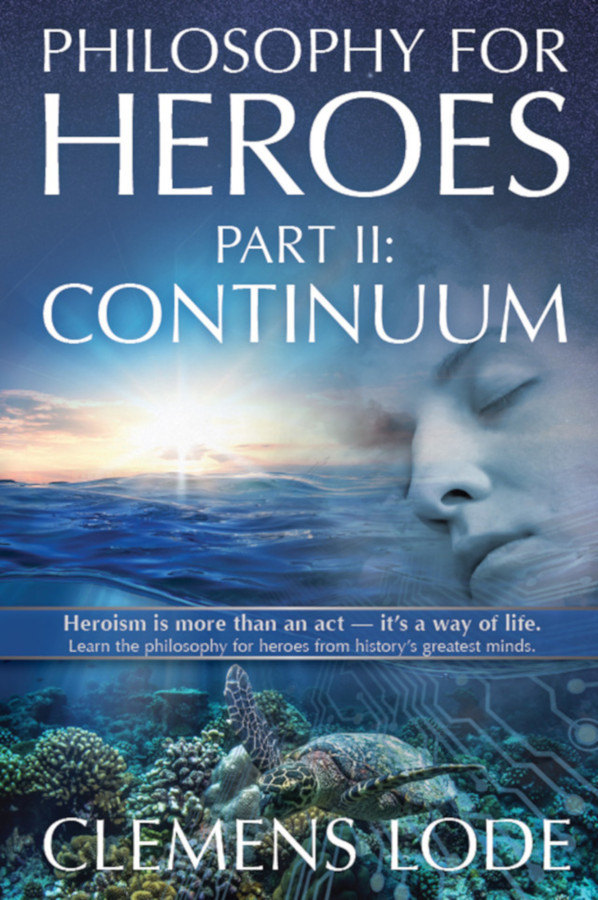
\includegraphics{images/pfh2-cover-900.jpg}
\label{c1_pfh:fig}
\end{figure}

\begin{figure}[H]\centering

\includegraphics{images/Agile_5-11-17_HiRes2-900.jpg}~
\includegraphics{images/KanbanFront_6-28-17_HiRes-900.jpg}
\label{c1_projectmanagement:fig}
\end{figure}

% Remove the following section if you only want to show your covers, replace with your own book descriptions. The example entries are books I have written using this template.


Here are other books by YOUR NAME. All share the topics of philosophy, psychology, leadership, and project management.

\begin{setlength}{\leftmargin}{1cm} 
\begin{description}\setlength{\itemsep}{-5pt}

\item[Better Books with LaTeX] In \citetitle{BBWL}\index{@\citetitle{BBWL}}\ifxetex\else{} \citep{BBWL}\fi, author Clemens Lode provides you a short-cut into the world of book publishing with \LaTeX{}. It is not a book that just lists all the commands and then leave you alone, it guides you alongside a fully working template (this one!).

\item[Part I: Knowledge.] In \citetitle{PFH1E}\index{@\citetitle{PFH1E}}\ifxetex\else{} \citep{PFH1E}\fi, the first book in this four-book series, author Clemens Lode takes the reader on a journey, examining the foundations of knowledge. What is the basis of our understanding of the world? How does society define a ``hero''? How do basic skills, such as language and mathematics, train our way of thinking and reasoning?

\item[Part II: Continuum.] Beyond the static world of the first book, \citetitle{PFH2E}\index{@\citetitle{PFH2E}}\ifxetex\else{} \citep{PFH2E}\fi{} looks at gradual transitions from one condition to the next. Where do we come from? Why is there something rather than nothing? What is the source of our creativity? How can the study of natural sciences help us to understand who we are?

\item[Scrum Your Jira!] In \citetitle{scrum-your-jira}\index{@\citetitle{scrum-your-jira}}\ifxetex\else{} \citep{scrum-your-jira}\fi, author Clemens Lode challenges two illusions that can get in the way of your company's road to being truly Agile: first, that your Scrum is ``special,'' and second, that you can hide behind project management software. Jira is powerful\emdash{}and this book will show you how to use it more effectively\emdash{}but it makes it easy to forget that the first idea of Agile is: Individuals and interactions over processes and tools.

\item[Kanban Remastered] StarCraft, the most popular real-time strategy game of all time, is also all about producing and deploying just as many game units at just the right time. This book is about the relationship of StarCraft and Kanban. When your team knows StarCraft but not Kanban, \citetitle{kanban-remastered}\index{@\citetitle{kanban-remastered}}\ifxetex\else{} \citep{kanban-remastered}\fi{} will provide you with a series of analogies to allow a better and easier understanding of Agile principles. It is written in a light-hearted tone, similar to how you might chat with a fellow coach about your Agile experiences implementing Kanban, taking for granted that you have experience with StarCraft.

\end{description}
\end{setlength}\blankpage

% list of uncited references that are still good reads (only for printed PDF)
\ifxetex
	%%%%%%%%%%%%%%%%%%%%%%%%%%%%%%%%%%%%%
% Read the /ReadMeFirst/ReadMeFirst.tex for an introduction. Check out the accompanying book "Better Books with LaTeX" for a discussion of the template and step-by-step instructions. The template was originally created by Clemens Lode, LODE Publishing (www.lode.de), mail@lode.de, 8/17/2018. Feel free to use this template for your book project!
%%%%%%%%%%%%%%%%%%%%%%%%%%%%%%%%%%%%%

% list of uncited references that are still good reads (only for printed PDF). Replace the citations accordingly.

\nocite{PFH1E}
\nocite{PFH2E}
\nocite{PFH3E}
\nocite{PFH4E}

\printbibliography[keyword=recommendedEN, title={Recommended Reading}]\blankpage
\fi

%%%%%%%%%%%%%%%%%%%%%%%%%%%%%%%%%%%%%
% Read the /ReadMeFirst/ReadMeFirst.tex for an introduction. Check out the accompanying book "Better Books with LaTeX" for a discussion of the template and step-by-step instructions. The template was originally created by Clemens Lode, LODE Publishing (www.lode.de), mail@lode.de, 8/17/2018. Feel free to use this template for your book project!
%%%%%%%%%%%%%%%%%%%%%%%%%%%%%%%%%%%%%


% Upload hires (author_highres.png) and lowres picture (author.jpg) of author into images folder, and uncomment the 5 includegraphics lines.
% Replace quotation text
% Add text describing your motivation, your professional background, what you are currently doing, and how to connect with you.

\begin{chapterpage}{
	{The Author}
}{p1_the-author:cha}

\vspace*{\fill}

\begin{center}

%\ifxetex
%	\includegraphics[width=.7\textwidth]{images/author_hires.png}
%\else
%	\includegraphics{images/author.jpg}
%\fi

\end{center}
\vspace*{\fill}

\begin{myquotation} Viver, morrer, renascer. Progredir sempre. Amar a Deus sobre todas as coisas e ao próximo como a Si mesmo. Buscai em primeiro lugar o Reino de Deus e tudo o mais vos será acrescentado.\end{myquotation}

\end{chapterpage}

Describe your dreams, what goals you have in life, where you went to school or studied, and what job you currently work or worked in the past. Make clear what motivated you to start writing. Finally, add contact points where people can connect with you (mail, Facebook, Twitter, etc.). 
\blankpage
%%%%%%%%%%%%%%%%%%%%%%%%%%%%%%%%%%%%%
% Read the /ReadMeFirst/ReadMeFirst.tex for an introduction. Check out the accompanying book "Better Books with LaTeX" for a discussion of the template and step-by-step instructions. The template was originally created by Clemens Lode, LODE Publishing (www.lode.de), mail@lode.de, 8/17/2018. Feel free to use this template for your book project!
%%%%%%%%%%%%%%%%%%%%%%%%%%%%%%%%%%%%%

% Use this chapter to summarize what you have learned while writing the book. This helps you to write better books in the future and might be interesting for the reader to know about how the book came about.

\begin{chapterpage}{The Book's Story}{p2_booksstory:cha}

% Add a quotation to set the team for your lessons learned
Este livro nasceu da proposta da minha psicóloga Fernanda Volpe Cunha de eu escrever sobre meus pensamentos e sentimentos para poder levar a ela todo esse conteúdo. Aconteceu que foi mais que isso pois os assuntos pessoais levo a ela contudo os de interesse geral partilho aqui.

Acredito piamente que as pessoas precisam desenvolver senso crítico-filosófico e precisam de auto-conhecimento. O que escrevo aqui, não tenho a pretensão de afirmar que é a verdade absoluta pois verdade absoluta só Deus conhece. Mas cada um refletindo sobre os conteúdos, seja concordando ou discordando, encontrará meios de desenvolver-se como uma musculação para a mente e então ficará mais forte para a Vida, esse o objetivo da presente obra.

\end{chapterpage}



\blankpage


% switch back to basic chapter design
%  Reset the chapter design to a basic one (no box, just underlined chapter title---used for the back and front matter)

\renewcommand*\chapterheadstartvskip{\vspace*{-3\topskip}} 
\renewcommand*\chapterheadendvskip{
  \vskip-.5\baselineskip
  \noindent
  {\color{gray}\rule{\linewidth}{2pt}}
  \par}
\renewcommand*\chapterformat{}
\renewcommand*{\chapterpagestyle}{empty}

% needs to be in curly braces because parskip change.
{
\parskip=5pt
%%%%%%%%%%%%%%%%%%%%%%%%%%%%%%%%%%%%%
% Read the /ReadMeFirst/ReadMeFirst.tex for an introduction. Check out the accompanying book "Better Books with LaTeX" for a discussion of the template and step-by-step instructions. The template was originally created by Clemens Lode, LODE Publishing (www.lode.de), mail@lode.de, 8/17/2018. Feel free to use this template for your book project!
%%%%%%%%%%%%%%%%%%%%%%%%%%%%%%%%%%%%%

\chapter{Reflection}

\begin{problem}
Introductory text about what this section is about. For example, describe that this is a summary of all the problem boxes throughout the book and point to an online forum where readers can discuss them.\end{problem}

% Reset formatting
\setlength{\parindent}{0.0cm}
\renewcommand{\index}[1]{}
\renewenvironment{problem}[1][]{$\bullet$\ #1}
\footnotesize 


\section*{Replace with Your First Chapter}
% Add questions located in your first chapter.
\begin{problem}What is LaTeX?\end{problem}


\section*{Replace with Your Second Chapter}
% Add questions located in your second chapter.
\begin{problem}What is LaTeX?\end{problem}


\section*{Replace with Your Third Chapter}
% Add questions located in your third chapter.
\begin{problem}What is LaTeX?\end{problem}
\newpage
%%%%%%%%%%%%%%%%%%%%%%%%%%%%%%%%%%%%%
% Read the /ReadMeFirst/ReadMeFirst.tex for an introduction. Check out the accompanying book "Better Books with LaTeX" for a discussion of the template and step-by-step instructions. The template was originally created by Clemens Lode, LODE Publishing (www.lode.de), mail@lode.de, 8/17/2018. Feel free to use this template for your book project!
%%%%%%%%%%%%%%%%%%%%%%%%%%%%%%%%%%%%%

\chapter{Eureka!}

\begin{idea}
Introductory text about what this section is about. For example, describe that this is a summary of all the idea boxes throughout the book.\end{idea}

% reformat idea boxes
\renewenvironment{idea}[1][]{$\bullet$\ #1}
%\setlength{\parindent}{0.7cm}

% deactivate indexing of idea boxes to prevent duplicates
\ifxetex
	\renewcommand{\index}{}
\fi

\section*{Replace with Your First Chapter}
% Add ideas located in your first chapter.
\begin{idea}
\LaTeX{} is a document preparation system.
\end{idea}

\section*{Replace with Your Second Chapter}
% Add ideas located in your second chapter.
\begin{idea}
\LaTeX{} is a document preparation system.
\end{idea}

\section*{Replace with Your Third Chapter}
% Add ideas located in your third chapter.
\begin{idea}
\LaTeX{} is a document preparation system.
\end{idea}\newpage
\parskip=0pt
%%%%%%%%%%%%%%%%%%%%%%%%%%%%%%%%%%%%%
% Read the /ReadMeFirst/ReadMeFirst.tex for an introduction. Check out the accompanying book "Better Books with LaTeX" for a discussion of the template and step-by-step instructions. The template was originally created by Clemens Lode, LODE Publishing (www.lode.de), mail@lode.de, 8/17/2018. Feel free to use this template for your book project!
%%%%%%%%%%%%%%%%%%%%%%%%%%%%%%%%%%%%%


% If you have added or removed any entries in the glossary directory, add them here. If a letter is missing, add a new \section*{} with the letter.

\chapter{Glossary}

% Special formatting for glossary 
\setlength{\parindent}{0.7cm}
\renewcommand{\index}[1]{}
\renewenvironment{definition}[2][]{\textbf{#2}\ $\bullet$\ #1}
\footnotesize
%\ifxetex
%	\titlespacing*{\section}{0pt}{3.5ex plus 1ex minus .2ex}{2.3ex plus .2ex}
%\fi

\vspace{20pt}


\section*{E}
\begin{multicols}{2}
\begin{definition}{Entity}\index{entity|textbf} An \emph{entity} is a ``thing'' with properties (an identity). For example, a plant produces oxygen, a stone has a hard surface, etc.).\end{definition}
\end{multicols}

\section*{I}
\begin{multicols}{2}
\begin{definition}{Identity}\index{identity|textbf} An \emph{identity} is the sum total of all properties\index{entity!property} of an entity (e.g., weight: 160 pounds, length: 6 feet, has a consciousness, etc.).\end{definition}

\end{multicols}

\section*{L}
\begin{multicols}{2}
\begin{definition}{LaTeX}\index{latex|textbf} \LaTeX{} is a document preparation system.\end{definition}
\end{multicols}

\section*{P}
\begin{multicols}{2}
\begin{definition}{Property}\index{entity!property|textbf} A \emph{property} refers to the manner in which an entity (or a process) affects other entities (or other processes) in a certain situation (e.g., mass, position, length, name, velocity, etc.).\end{definition}
\end{multicols}\newpage
% add separate quotations page (sources in the e-book are already included in the text body)
\ifxetex
	%%%%%%%%%%%%%%%%%%%%%%%%%%%%%%%%%%%%%
% Read the /ReadMeFirst/ReadMeFirst.tex for an introduction. Check out the accompanying book "Better Books with LaTeX" for a discussion of the template and step-by-step instructions. The template was originally created by Clemens Lode, LODE Publishing (www.lode.de), mail@lode.de, 8/17/2018. Feel free to use this template for your book project!
%%%%%%%%%%%%%%%%%%%%%%%%%%%%%%%%%%%%%

% quotation sources (only for print PDF where the source is not directly mentioned in the text body).

\chapter{Quotation Sources}

\setlength{\parindent}{0pt}
\footnotesize

\babelDE{\textbf{\pageref{gogh-sky-quote}:} \cite[vgl.][S.~23--24]{ifyouwanttowrite}}
\babelEN{\textbf{\pageref{gogh-sky-quote}:} \cite[pp.~23--24]{ifyouwanttowrite}}\par
\fi
}

%%%%%%%%%%%%%%%%%%%%%%%%%%%%%%%%%%%%%
% Read the /ReadMeFirst/ReadMeFirst.tex for an introduction. Check out the accompanying book "Better Books with LaTeX" for a discussion of the template and step-by-step instructions. The template was originally created by Clemens Lode, LODE Publishing (www.lode.de), mail@lode.de, 8/17/2018. Feel free to use this template for your book project!
%%%%%%%%%%%%%%%%%%%%%%%%%%%%%%%%%%%%%


% Command to add some text into the bibliography (between the title and the list of referenced books)
% See https://tex.stackexchange.com/questions/197061/text-between-index-or-bibliography-title-and-content
\newcommand{\bibpreface}[1]{\patchcmd{\thebibliography}{\list}{#1\list}{}{}}

\bibpreface{Write here the preface of your list of recommended reading titles. Delete this line to have no preface for this section.}

\ifxetex
	\printbibliography
\else
	\newpage
	\bibliographystyle{plainnat}
	\bibliography{bibliography/english}
\fi


% ---------- Appendix
\appendix
    
%%%%%%%%%%%%%%%%%%%%%%%%%%%%%%%%%%%%%
% Read the /ReadMeFirst/ReadMeFirst.tex for an introduction. Check out the accompanying book "Better Books with LaTeX" for a discussion of the template and step-by-step instructions. The template was originally created by Clemens Lode, LODE Publishing (www.lode.de), mail@lode.de, 8/17/2018. Feel free to use this template for your book project!
%%%%%%%%%%%%%%%%%%%%%%%%%%%%%%%%%%%%%

% the index page, only for printed PDF

\ifxetex	
	\pagestyle{empty}
	\appendix
	\indexprologue{Replace index prologue with an own introduction of how to contact you when there is an errata concerning the index.}
    \printindex
\fi

%%%%%%%%%%%%%%%%%%%%%%%%%%%%%%%%%%%%%
% Read the /ReadMeFirst/ReadMeFirst.tex for an introduction. Check out the accompanying book "Better Books with LaTeX" for a discussion of the template and step-by-step instructions. The template was originally created by Clemens Lode, LODE Publishing (www.lode.de), mail@lode.de, 8/17/2018. Feel free to use this template for your book project!
%%%%%%%%%%%%%%%%%%%%%%%%%%%%%%%%%%%%%


% Replace it with your own call to action if you like, or use the default text.

\chapter{An Important Final Note}

% Only show for e-books.
\ifxetex \else \textit{If you want to rate this e-book, please also add a short text comment. Without a text comment, your star rating will be invisible on the Amazon website and count only as an indicator for further recommendations on Amazon. Thanks!}\fi

Writers are not performance artists. While there are book signings and public readings, most writers (and readers) follow their passion alone in their homes.

\textit{What applause is for the musician, \textbf{reviews} are for the writer.} 

\textit{Books create a community among readers}; you can share your thoughts among all those who will or have read the book.

\textbf{Leave a thoughtful honest review and help me to create such a community on the platform on which you have acquired this book.} \textit{What did you like, what can be improved? To whom would you recommend it?} 

Thank you, also in the name of all the other readers who will be able to better decide whether this book is right for them or not! A positive review will increase the reach of the book, a negative review will improve the quality of the next book. I welcome both!
%%%%%%%%%%%%%%%%%%%%%%%%%%%%%%%%%%%%%
% Read the /ReadMeFirst/ReadMeFirst.tex for an introduction. Check out the accompanying book "Better Books with LaTeX" for a discussion of the template and step-by-step instructions. The template was originally created by Clemens Lode, LODE Publishing (www.lode.de), mail@lode.de, 8/17/2018. Feel free to use this template for your book project!
%%%%%%%%%%%%%%%%%%%%%%%%%%%%%%%%%%%%%

% Replace quote

\newpage
\thispagestyle{empty}
\vspace*{\fill}
\hfill

\babelEN{\begin{myquotation} Deus abençoe a todos\par\mbox{}\hfill \emdash{}Geraldo Cesar Cantelli\end{myquotation}}

\end{document}
\balance